%% 
%% Copyright 2019-2024 Elsevier Ltd
%% 
%% Version 2.4
%% 
%% This file is part of the 'CAS Bundle'.
%% --------------------------------------
%% 
%% Adapted from `cas-dc-sample.tex`.
%% Manuscript content filled from `main.tex`.
%% 

% Applied Soft Computing / Elsevier double-column working copy.
% Keep Manuscript.tex as the single-column editing master.
\documentclass[a4paper,fleqn]{cas-dc}

%\usepackage[authoryear,longnamesfirst]{natbib}
%\usepackage[authoryear]{natbib}
\usepackage[numbers,sort&compress]{natbib}
%\biboptions{sort&compress}

%\usepackage[authoryear,longnamesfirst]{natbib}
%\usepackage[authoryear]{natbib}
%\usepackage[numbers,sort&compress]{natbib}

\usepackage{amsmath}
\usepackage{amssymb}
\usepackage{amsthm}
\usepackage{booktabs}
\usepackage{multirow}
\usepackage{graphicx}
\usepackage{makecell}
\usepackage{tabularx}
\usepackage{array}
\usepackage{algorithm}
\usepackage{algpseudocode}
\usepackage{microtype}
\usepackage{subcaption}
\usepackage{xurl}

\usepackage[section]{placeins}
\usepackage{cleveref}

\theoremstyle{plain}
\newtheorem{proposition}{Proposition}[section]
\theoremstyle{definition}
\newtheorem{definition}{Definition}

%%%Author definitions
\def\tsc#1{\csdef{#1}{\textsc{\lowercase{#1}}\xspace}}
\tsc{WGM}
\tsc{QE}
\tsc{EP}
\tsc{PMS}
\tsc{BEC}
\tsc{DE}
%%%

\begin{document}
\let\WriteBookmarks\relax
\def\floatpagepagefraction{1}
\def\textpagefraction{.001}

\shorttitle{DRL-Based Pinning Synchronization of Hopfield Networks}
\shortauthors{Huang et~al.}


\title [mode = title]{Deep-Reinforcement-Learning-Based Single-Input Pinning Synchronization of Hopfield Chaotic Neural Networks with an Application to Image Encryption}

\author[1]{Yan'an Huang}
\fnmark[1]
\ead{6253111028@stu.jiangnan.edu.cn}
\author[1]{Zixuan Qiao}
\fnmark[1]
\ead{6253114027@stu.jiangnan.edu.cn}
\author[2]{Jiabing Zhu}
\ead{zhujb@inspur.com}
\author[1]{Weiye Wang}
\ead{6243115018@stu.jiangnan.edu.cn}
\author[1]{Xiaoyan Sun}
\ead{xysun78@126.com}
\author[3]{Chenchen Yu}
\ead{m15866813396@163.com}
\author[1]{Jie Wu}
\cormark[1]
\author[4]{Ru-ru Ma}
\cormark[1]
\affiliation[1]{
	organization={School of Artificial Intelligence and Computer Science, Jiangnan University},
	city={Wuxi},
	postcode={214122},
	country={China}
}
\affiliation[2]{
	organization={Inspur Software Group Co., Ltd},
	city={Jinan},
	postcode={250000},
	country={China}
}
\affiliation[3]{
	organization={Qingdao Haier Air Conditioner Electronic Co., Ltd},
	city={Qingdao},
	postcode={266101},
	country={China}
}
\affiliation[4]{
	organization={School of Mathematics and Physics, Suzhou University of Science and Technology},
	city={Suzhou},
	postcode={215009},
	country={China}
}

\fntext[1]{These authors contributed equally to this work.}
\cortext[cor1]{Corresponding authors. E-mail addresses: jiewu20@jiangnan.edu.cn (J. Wu); maruru7271@126.com (R. Ma).}

\begin{abstract}
A single control input limits where feedback enters a chaotic system, but leaves open which variables the controller should observe. This study investigates how these two design choices interact in the synchronization of a continuous-time Hopfield network. Proximal policy optimization (PPO) is used to learn bounded feedback, with local node-screening indicators and a state-boundedness analysis guiding the assessment. The central finding is that observation composition can matter as much as input dimension: changing the coordinate subset improves synchronization at Node 2 but worsens it at Node 3, despite retaining the same observation size. A targeted soft actor-critic (SAC) comparison reproduces this direction of change, while revealing algorithm-dependent differences in control effort. An accuracy-constrained screening example translates the observed preferences into choices within a fixed candidate pool. Comparisons across all actuator subsets further show the cost of restricting control to one node: favorable multi-input configurations improve full-horizon accuracy at greater total effort, whereas steady-state precision follows a different ordering. Traditional-controller and SAC benchmarks place these findings in the context of controller-dependent accuracy--effort tradeoffs. An image encryption and decryption demonstration provides an application of the synchronized trajectories. Together, the results show why actuator placement, feedback information, and control effort should be considered jointly when designing single-input synchronization for the studied network.
\end{abstract}

\begin{keywords}
Image encryption \sep
Synchronization \sep
Deep reinforcement learning \sep
Neural network
\end{keywords}
\maketitle

\section{Introduction}
\setlength{\emergencystretch}{2em}
\label{sec:introduction}

Nonlinear dynamical systems and chaotic phenomena have attracted enduring interest across physics, mathematics, and engineering sciences~\cite{strogatz2018nonlinear,boccaletti2006complex,izhikevich2007dynamical}, primarily due to their hallmark property: extreme sensitivity to initial conditions, whereby infinitesimal state discrepancies amplify exponentially over time into pseudorandom, unpredictable trajectories. This intrinsic unpredictability long rendered chaotic systems difficult to regulate, until the pioneering discovery of drive--response synchronization by Pecora and Carroll in 1990~\cite{pecora1990synchronization}. Their seminal work demonstrated that two coupled or appropriately controlled chaotic systems can achieve coherent dynamical evolution, unlocking widespread applications in secure communication~\cite{koronovskii2010on,argyris2005chaos,vanwiggeren1998communication}, cooperative network control~\cite{wen2021coordination,olfati2007consensus}, and image encryption~\cite{zia2022survey,xu2014image}. Over the past decades, diverse synchronization regimes—such as complete synchronization~\cite{lin2005complete}, generalized synchronization~\cite{kocarev1996generalized}, and phase synchronization~\cite{guan2005phase}—have been extensively investigated through traditional model-based control strategies~\cite{ott1990controlling,boccaletti2000control}, including linear feedback~\cite{yassen2005controlling}, adaptive control~\cite{wang2003feedback}, sliding-mode control~\cite{feki2009sliding,su2021fixed,mobayen2018chaos}, impulsive control~\cite{li2005impulsive}, and pinning control~\cite{chen2014pinning}.

In recent years, secure image transmission has emerged as a prominent application scenario where chaos dynamics and synchronization play an indispensable role. In distributed communication environments—such as remote sensing, telemetry links, and distributed astronomical observation networks (e.g., Very Long Baseline Interferometry arrays)~\cite{thompson2017interferometry}—large volumes of sensitive and high-value scientific imagery must be transmitted across open and potentially untrusted channels. These transmission scenarios are vulnerable to eavesdropping and data interception, while simultaneously operating under stringent physical constraints: limited channel bandwidth, constrained terminal computing resources, and strict energy budgets. Such requirements necessitate lightweight, low-cost, and computationally efficient encryption frameworks capable of securing high-value visual data without imposing heavy communication or computational burdens.

Chaotic systems are naturally endowed with properties that align with cryptographic primitives: ergodicity, broadband continuous spectra, spatiotemporal pseudorandomness, and extreme initial-state sensitivity~\cite{zia2022survey}. In conventional cryptography, the distribution of secret keys or the transmission of pseudorandom keystreams over public channels inevitably creates key-distribution bottlenecks and security vulnerabilities. In contrast, drive--response chaotic synchronization establishes a ``zero-key-transmission'' cryptographic paradigm: the transmitter (drive system) locally generates a continuous chaotic trajectory to construct the encryption keystream, while the receiver (response system) independently reconstructs the identical chaotic trajectory through synchronization. Consequently, the need to transmit or expose the keystream across vulnerable communication channels is eliminated. To generate cryptographically robust keystreams, continuous-time Hopfield chaotic neural networks (CHNNs)~\cite{hopfield1984neurons,LI2013a} offer pronounced dynamical advantages over discrete toy maps (such as Logistic, Tent, or Arnold maps) and low-dimensional polynomial oscillators (such as Lorenz or Chen systems). Under finite-precision digital computation, discrete maps frequently suffer from dynamical degradation, short periodic orbits, and non-uniform state distributions, whereas low-dimensional polynomial oscillators exhibit relatively simple vector fields and limited topological complexity. In contrast, continuous-time Hopfield neural networks represent recurrent neuromorphic dynamical systems governed by saturating transcendental nonlinearities ($\tanh$) and interconnected by asymmetric synaptic weight matrices $W$. They generate rich multi-scroll chaotic attractors, broadband pseudorandom trajectories with high spatiotemporal uniformity, and elevated Shannon entropy~\cite{zheng2010double,bao2017numerical,mahmoud2021analysis}, thereby supplying high-complexity, continuous-state key material for image diffusion, permutation, and dynamic DNA coding.

However, translating chaotic synchronization into practical, resource-constrained image transmission encounters a critical control-theoretic and engineering bottleneck: actuation overhead and telemetry communication bandwidth. In a master--slave synchronization architecture, the drive and response systems are physically separated across distinct communication nodes. Conventional synchronization methods frequently rely on full-state or multi-input control architectures~\cite{yassen2005controlling,feki2009sliding,su2021fixed}, where control corrections are simultaneously applied to every state dimension. In real-time remote telemetry, transmitting multi-channel control signals or state corrections requires communication bandwidth that scales directly and linearly with the actuation dimension. For an $n$-dimensional chaotic system, multi-input control multiplies the required telemetry traffic by $n$-fold, while simultaneously requiring multiple physical actuators, digital-to-analog converters, and driving circuits. For the three-dimensional Hopfield neural network investigated in this study, full-state control would require three independent actuator channels and triple the telemetry bandwidth. To address this challenge, this paper investigates an underactuated single-input pinning control strategy, in which only a single scalar control signal is injected into one selected node of the response system. By restricting actuation to a single dimension, the required control telemetry bandwidth, driver circuitry, and physical actuation cost are reduced by 66.7\%, which is particularly advantageous for bandwidth-constrained remote transmission links.

Nevertheless, single-input pinning control presents significant control difficulties: because only one node is directly actuated, the control force must propagate to the remaining uncontrolled nodes solely through the internal recurrent synaptic connections ($W$) of the neural network. In continuous-time Hopfield networks, the synaptic weight matrix $W$ is intrinsically asymmetric, meaning that individual nodes occupy fundamentally unequal topological and dynamical positions. Certain nodes possess strong outgoing synaptic projections and weak transverse divergence, making them naturally favorable channels for control propagation; conversely, other nodes exhibit weak coupling or strongly divergent transverse directions, acting as structural underactuation bottlenecks. Consequently, the choice of pinning node is critical: applying control to different nodes yields markedly divergent synchronizability, convergence rates, and control effort. Traditional model-based controllers (such as linear feedback, LQR, and sliding-mode control)~\cite{wang2003feedback,li2005impulsive,chen2014pinning,mobayen2018chaos} rely on explicit linearizations or strict structural matchings; while they can stabilize locally favorable channels, they exhibit severe performance degradation, consume excessive control energy, or even fail when applied to structurally disadvantaged nodes or subjected to parameter mismatches and disturbances~\cite{zhang2011weak,cao2024synchronisation}. Deep reinforcement learning (DRL)~\cite{sutton2018reinforcement,mnih2015human,carlucho2020adaptive} offers a model-free, data-driven methodology to discover optimal nonlinear feedback policies directly from dynamical interactions, as evidenced in recent chaos control studies~\cite{bucci2019control,vashishtha2020restoring,han2021control,cheng2023deep,cheng2025generalized,yau2024ppo,xu2025ppo,jin2025Deep,weissenbacher2025reinforcement}. However, how recurrent network topology dictates single-input pinning feasibility, and more importantly, \emph{where} DRL policies provide decisive advantages over classical feedback across different topological channels, remains an unaddressed research gap.

Furthermore, an essential gap exists between continuous chaotic synchronization and discrete image encryption in the current literature: synchronization studies typically terminate at continuous error convergence ($\|\mathbf{e}(t)\| \to 0$) without verifying downstream application viability, whereas image encryption studies often assume perfectly synchronized keys as an abstract given. In physical implementation, continuous chaotic trajectories must be discretized and quantized into finite integer keystreams (such as DNA encoding rules and diffusion masks). Because quantization partitions continuous state space into discrete bins, any residual synchronization error exceeding the bin boundaries will trigger key misalignments, causing catastrophic error propagation and complete decryption failure. Therefore, achieving rapid, high-precision, low-residual synchronization under constrained single-input actuation is not an isolated control benchmark, but an indispensable physical prerequisite for lossless image reconstruction.

Motivated by these considerations and research gaps, this paper investigates the single-input pinning synchronization of continuous-time Hopfield chaotic neural networks and its application to secure image encryption. A unified DRL-based framework using proximal policy optimization (PPO) is developed to synthesize constrained nonlinear pinning policies. A multi-index local analysis is first formulated to establish a theoretical pre-screening ranking across candidate nodes. Systematic comparative experiments are then conducted across all physical dimensions (Nodes 1, 2, and 3) under nominal synchronization, parameter mismatch, global impulse disturbances, Gaussian noise, and partial-observation constraints against tuned classical baselines. Crucially, our findings resolve the relationship between topological suitability and learning efficacy: while the locally preferred Node 3 achieves low error under both classical and learning control, PPO demonstrates its most decisive and dramatic advantage on the structurally difficult channel (Node 2)—slashing the post-impulse recovery error by 62.6\% and control energy by 68.6\% compared to linear feedback. Finally, the synchronized trajectories are deployed in an end-to-end image encryption pipeline employing Logistic-map diffusion and three-round asymmetric DNA coding over the full symmetric group $S_4$, demonstrating 100\% loss-free image recovery and near-ideal cryptographic security.

The primary contributions of this paper are summarized as follows:
\begin{itemize}
	\item \textbf{Actuation-Minimal Underactuated Synchronization Architecture}: A single-input scalar pinning control framework is formulated for three-dimensional continuous-time Hopfield chaotic neural networks. By actuating only a single physical node, the control telemetry bandwidth and actuator hardware overhead are reduced by 66.7\% compared to conventional multi-input control, making it uniquely suited for bandwidth-constrained remote data links.

	\item \textbf{Multi-Index Topological Ranking of Pinning Channels}: A comprehensive local ranking framework combining the maximum conditional Lyapunov exponent (MCLE), Riccati-based optimal regulation cost, feedback gain norm, and local control propagation index is established. This framework reveals how asymmetric synaptic coupling $W$ governs node-wise controllability and observation demand prior to policy training.

	\item \textbf{Identification of the Node-Dependent DRL Learning Advantage}: Systematic comparative evaluations under parameter mismatch, global impulse disturbances, and persistent stochastic noise reveal that while Node 3 is topologically favorable where classical feedback suffices, PPO's true strength is unlocked on the structurally disadvantaged channel (Node 2)—achieving a 62.6\% reduction in post-disturbance error and a 68.6\% reduction in control energy over linear feedback, thereby clarifying the distinction between the ``easiest node'' and the ``largest benefit from machine learning.''

	\item \textbf{End-to-End Cryptographic Reversibility and Security Validation}: An end-to-end image encryption scheme is developed using synchronized Hopfield trajectories, Logistic-map diffusion, and three-round asymmetric DNA coding over the full symmetric group $S_4$. The direct causal relationship between continuous synchronization residual and discrete key-stream consistency is rigorously demonstrated, achieving 100\% pixel-level lossless decryption, near-optimal information entropy (7.999), and adjacent-pixel correlation near zero ($<0.023$).
\end{itemize}

The remainder of this paper is organized as follows. Section~\ref{sec:preliminaries} introduces the continuous-time Hopfield chaotic neural network and formulates the single-input pinning synchronization problem. Section~\ref{sec:ppo_pinning_method} presents the local pinning-node selection analysis and the DRL-based control framework implemented by PPO. Section~\ref{sec:experiments} reports the experimental setup, results, and discussion. Section~\ref{sec:image_encry} presents the application in image encryption. Finally, Section~\ref{sec:conclusion} concludes this paper and outlines possible future work.

\section{Preliminaries}
\label{sec:preliminaries}
Hopfield's continuous neural network model proposed in 1984~\cite{hopfield1984neurons} can be written as
\begin{equation}
	C_i \frac{du_i}{dt} = \sum_{j=1}^{n} T_{ij} V_j - \frac{u_i}{R_i} + I_i,
	\label{eq:hopfield_original_1}
\end{equation}
with the static nonlinear input--output mapping $V_i = g_i(u_i)$. Here, $u_i$ denotes the internal state variable of the $i$th neuron, $V_i$ is the neuron output, $C_i$ and $R_i$ represent the equivalent capacitance and resistance, respectively, $T_{ij}$ denotes the synaptic connection weight, and $I_i$ is the external bias input.

The symmetric coupling in the original Hopfield model supports an energy-based description of relaxation toward equilibrium. The chaotic network considered here instead uses asymmetric coupling, which removes that symmetry condition. Following the normalized Hopfield-type formulation in the control literature~\cite{LI2013a, mahmoud2021analysis}, we specify the drive dynamics first and then introduce the controlled response and synchronization error.

Introducing the parameter substitutions $a_i = \frac{1}{R_i C_i}$, $w_{ij} = \frac{T_{ij}}{C_i}$, and $b_i = \frac{I_i}{C_i}$, and assuming that all neurons share the same leakage coefficient ($a_i=1$), neglecting the constant bias term ($\mathbf{b}=\mathbf{0}$), and choosing $\tanh(\cdot)$ to characterize the saturating nonlinearity of the neuron output, one obtains the continuous-time Hopfield-type neural network model used in the subsequent analysis:
\begin{equation}
	\dot{\mathbf{x}}(t) = -\mathbf{x}(t) + W \tanh(\mathbf{x}(t)),
	\label{eq:hopfield_simplified_vector}
\end{equation}
Here, a node denotes one scalar state coordinate of the Hopfield network, rather than an entire chaotic oscillator. The drive and response are two copies of this network. The state vector is $\mathbf{x}(t) = [x_1(t), x_2(t), x_3(t)]^T$. Following the three-neuron Hopfield-type chaotic model studied in~\cite{mahmoud2021analysis}, in this paper, the network weight matrix is specified as
\begin{equation}
	W = \begin{bmatrix}
		-1.4 & 1.2 & -7.0 \\
		1.1 & 0.0 & 2.8 \\
		0.8 & -2.0 & 4.0
	\end{bmatrix}.
	\label{eq:weight_matrix}
\end{equation}

\begin{figure*}[pos=!t,width=\textwidth]
	\centering
	\setlength{\tabcolsep}{6pt}
	\begin{tabular}{cc}
		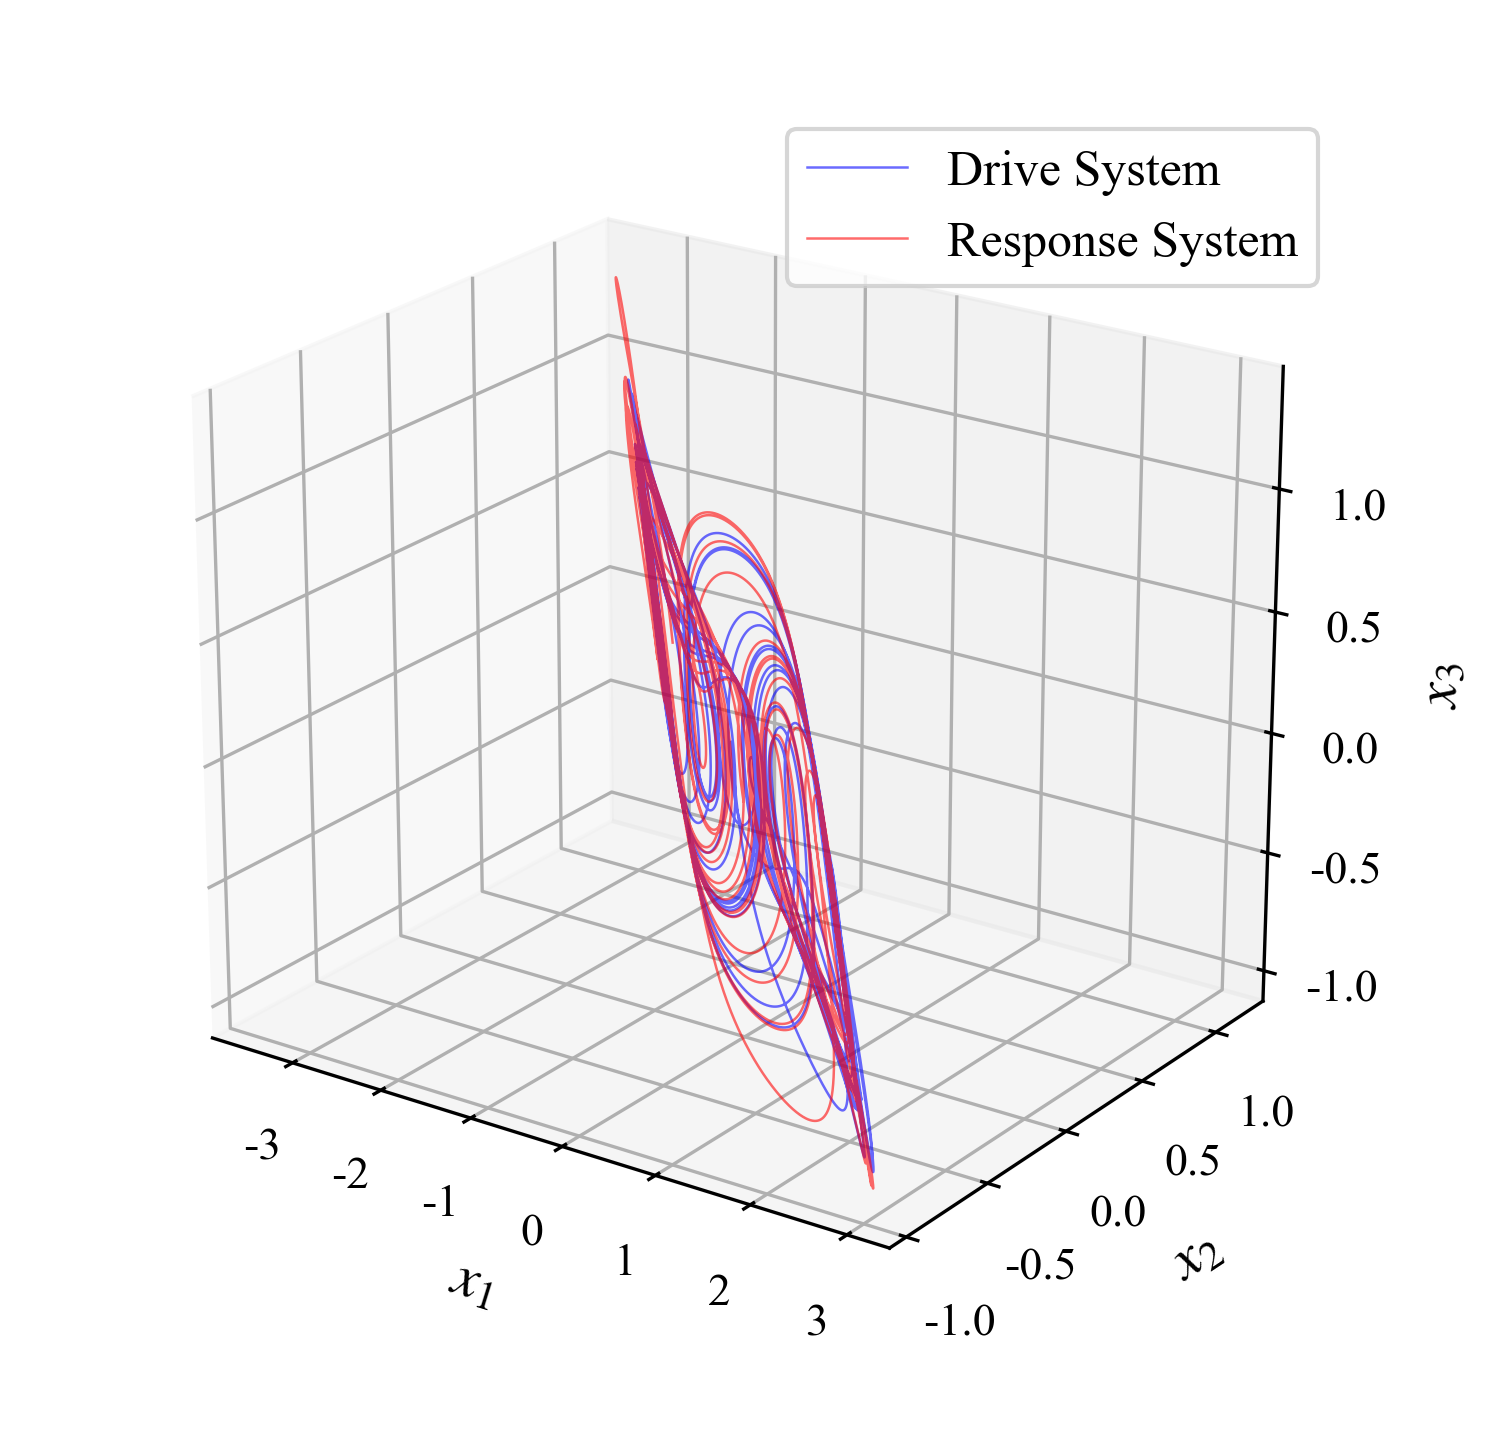
\includegraphics[width=0.47\textwidth]{figures/hopfield_phase_plane.png} &
		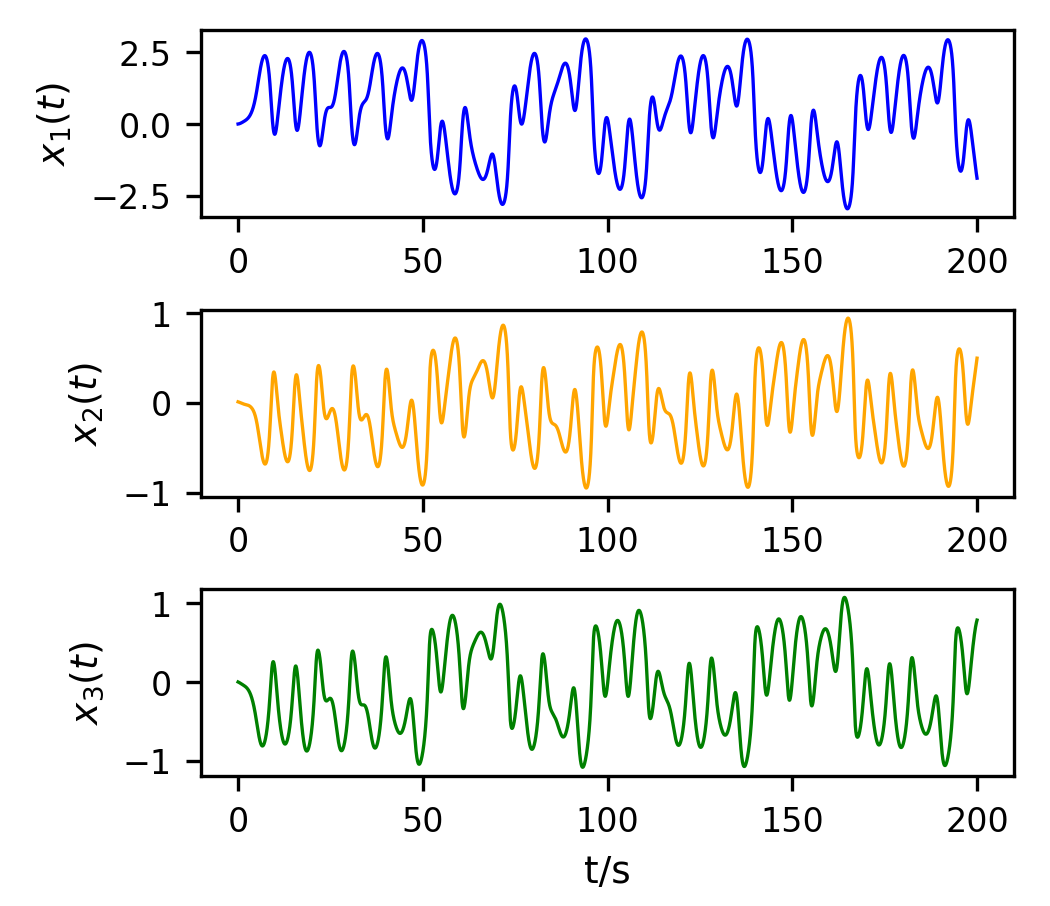
\includegraphics[width=0.47\textwidth]{figures/hopfield_chaos_trajectory.png} \\
		\small (a) Phase-space trajectories &
		\small (b) Time-domain trajectories
	\end{tabular}
	
	\caption{Uncontrolled phase-space trajectories of the drive and response Hopfield chaotic neural networks and time-domain state trajectories of the continuous-time Hopfield-type chaotic neural network.}
	\label{fig:hopfield_basic_dynamics}
\end{figure*}
%\begin{figure}[!ht]
%	\centering
%	
%	\begin{subfigure}[t]{0.47\linewidth}
%		\centering
%		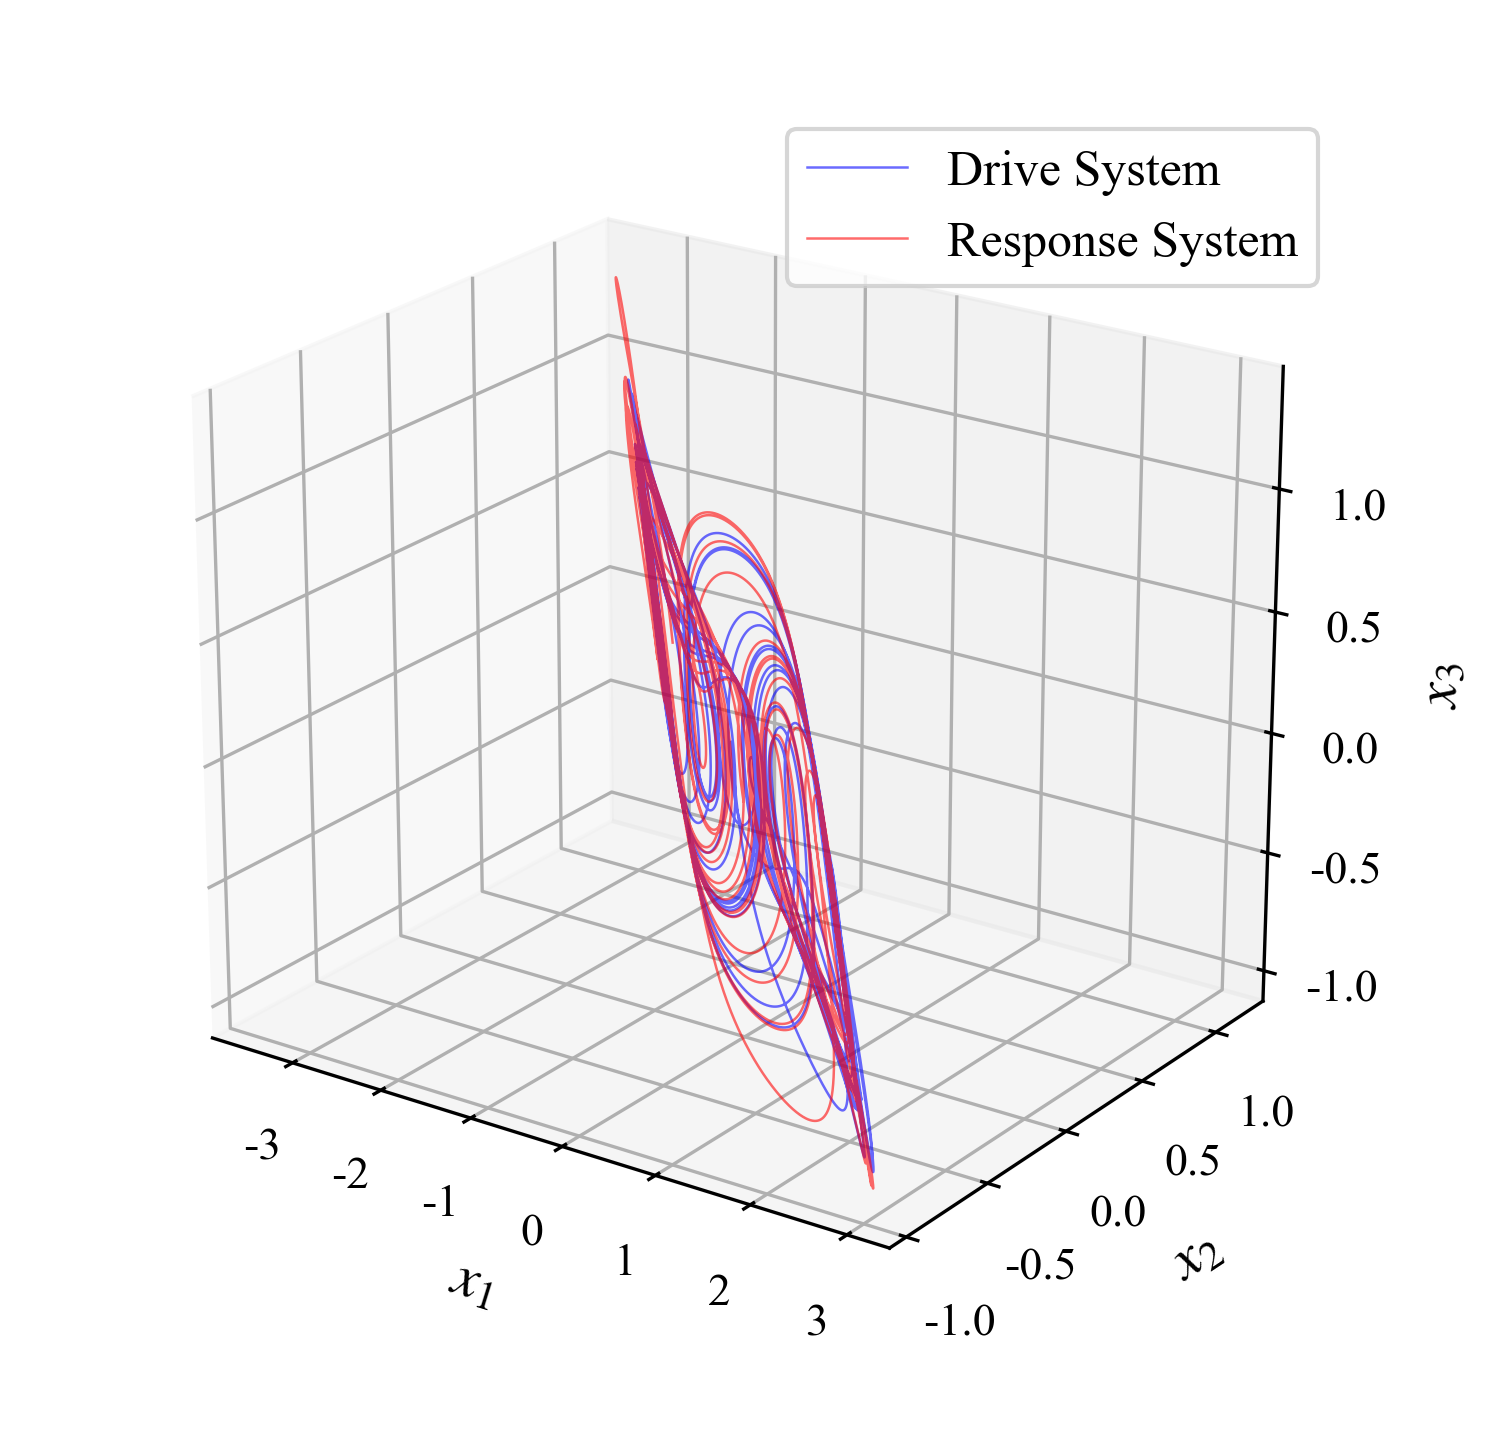
\includegraphics[width=\linewidth]{figures/hopfield_phase_plane.png}
%		\caption{Phase-space trajectories.}
%		\label{fig:uncontrolled_drive_response_phase}
%	\end{subfigure}
%	\hfill
%	\begin{subfigure}[t]{0.47\linewidth}
%		\centering
%		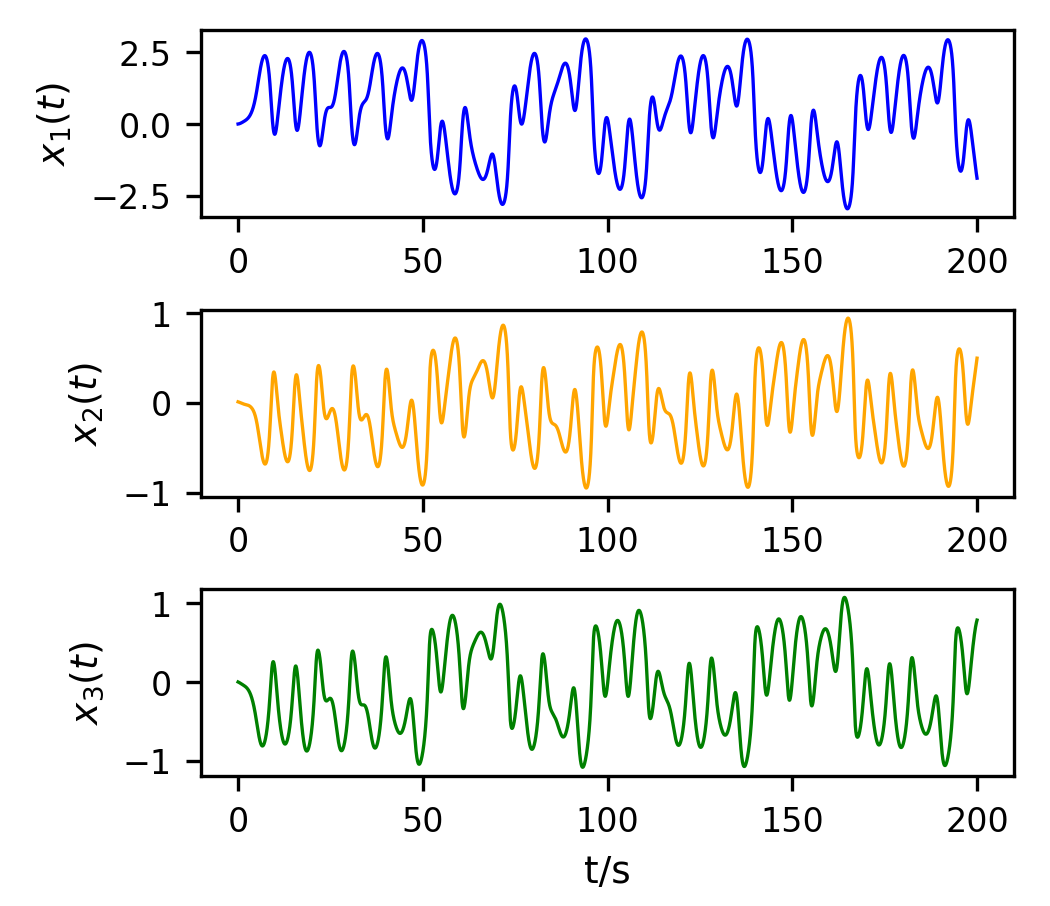
\includegraphics[width=\linewidth]{figures/hopfield_chaos_trajectory.png}
%		\caption{Time-domain trajectories.}
%		\label{fig:hopfield_chaos_trajectory}
%	\end{subfigure}
%	
%	\caption{Uncontrolled phase-space trajectories of the drive and response Hopfield chaotic neural networks and time-domain state trajectories of the continuous-time Hopfield-type chaotic neural network.}
%	\label{fig:hopfield_basic_dynamics}
%\end{figure}

The network in~\eqref{eq:hopfield_simplified_vector} is taken as the drive system. A single-input pinning controller is introduced into one selected response node, giving
\begin{equation}
	\dot{\mathbf{y}}(t) = -\mathbf{y}(t) + W_r \tanh(\mathbf{y}(t)) + B u(t),
	\label{eq:response_system}
\end{equation}
where $\mathbf{y}(t) \in \mathbb{R}^3$ is the state of the response system; $W_r$ is the weight matrix of the response system, which may differ from $W$ to represent parameter uncertainty; $u(t) \in \mathbb{R}$ is the scalar control input; and $B \in \mathbb{R}^{3 \times 1}$ is the pinning-node selection vector, which determines the specific physical node into which the control signal is injected. Only one of its three components is equal to 1, while the others are 0.

For this parameter setting, the initial condition 
$\mathbf{x}(0)=(0,0.01,0)^{\mathrm T}$, which has been used as a representative initial state in previous studies on Hopfield chaotic neural networks~\cite{mahmoud2021analysis}, is adopted to illustrate the basic chaotic behavior of the system. The fourth-order Runge--Kutta (RK4) trajectories illustrate the reported chaotic regime of this model. To further illustrate the uncontrolled drive--response behavior before applying the proposed pinning controller, two identical Hopfield chaotic neural networks are simulated with the same system parameters but different initial states sampled from $\mathrm{Uniform} ([-1,1]^3)$. As shown in Fig.~\ref{fig:hopfield_basic_dynamics}(a), the two trajectories evolve around the same double-scroll chaotic attractor but do not naturally synchronize.

The time-domain trajectories of $x_1(t)$, $x_2(t)$, and $x_3(t)$ obtained from the representative initial condition $\mathbf{x}(0)=(0,0.01,0)^{\mathrm T}$ are shown in Fig.~\ref{fig:hopfield_basic_dynamics}(b). The plotted irregular oscillations illustrate the drive dynamics in the reported chaotic regime.

Define the synchronization error as $\mathbf{e}(t) = \mathbf{y}(t) - \mathbf{x}(t)$. The ideal objective is vanishing synchronization error~\cite{boccaletti2002synchronization}. Subtracting the drive dynamics from the response dynamics gives
\begin{equation}
	\dot{\mathbf{e}}(t) = -\mathbf{e}(t) + W_r \tanh(\mathbf{y}(t)) - W \tanh(\mathbf{x}(t)) + B u(t).
	\label{eq:error_system_exact}
\end{equation}

The following definition mainly corresponds to the nominal synchronization control problem.
\begin{definition}
	For the drive system~\eqref{eq:hopfield_simplified_vector} and the response system with pinning control~\eqref{eq:response_system}, if under the action of the control law $u(t)$ one has $\lim_{t \to \infty} \| \mathbf{e}(t) \| = 0$, then the systems are said to achieve asymptotic synchronization.
\end{definition}

This definition provides the ideal reference. The implemented objective is to reduce synchronization error using a fixed actuator location and bounded input. Here, practical synchronization denotes the observed low-residual behavior over the reported testing windows; it is assessed by full-horizon and terminal error metrics rather than an assumed asymptotic limit. Section~\ref{subsec:boundedness_local_stability} separately examines boundedness and post-training trajectory sensitivity. Full observation is the default, and reduced policy inputs are evaluated as a separate experimental factor.

\section{PPO-Based Single-Input Pinning Control Method}
\label{sec:ppo_pinning_method}

The framework has three stages. Local dynamical and control indicators first identify candidate actuator locations. For each tested location, PPO learns a bounded scalar feedback policy from the nominal simulator. Finally, the trained policy with its parameters held fixed is evaluated using the implemented sampled dynamics, with state boundedness and local trajectory sensitivity treated separately. The indicators inform the choice of channels to investigate; they are not inputs to the policy or terms in the training reward.

\subsection{Local Pinning-Node Selection Analysis}
\label{subsec:local_node_selection}

Candidate nodes are compared using complementary local descriptions: transverse growth under ideal coordinate pinning, the LQR cost of a linear model evaluated at the origin, and an index based on the controllability matrix. These descriptions probe different aspects of actuator placement. They support qualitative screening before nonlinear evaluation, without assigning a combined numerical score.

For the local pinning-node analysis, we first consider the baseline identical-system setting, where the drive and response systems share the same weight matrix, i.e., $W_r=W$, and no external disturbance is imposed. When the synchronization error approaches zero, i.e., $\mathbf{e}\to \mathbf{0}$, the nonlinear term can be expanded to the first order around the synchronization manifold. This gives the following local linear approximation of the error system~\cite{slotine1991applied}:
\begin{equation}
	\dot{\mathbf{e}}(t)
	\approx
	\left[-I+WD(\mathbf{x}(t))\right]\mathbf{e}(t)
	+
	Bu(t),
	\label{eq:local_linear_error}
\end{equation}
where $I$ is the $3\times 3$ identity matrix, $W$ is the weight matrix of the drive system, $u(t)\in\mathbb{R}$ is the scalar control input, and $B\in\mathbb{R}^{3\times 1}$ is the control allocation vector indicating the node at which the control signal is injected. The diagonal matrix $D(\mathbf{x})$ is composed of the derivatives of the activation function:
\begin{equation}
	D(\mathbf{x})
	=
	\mathrm{diag}
	\left(
	1-\tanh^2(x_1),
	1-\tanh^2(x_2),
	1-\tanh^2(x_3)
	\right),
	\label{eq:D_matrix}
\end{equation}
where $x_1$, $x_2$, and $x_3$ are the state variables of the drive system.

For single-input pinning control, different node selections correspond to different control allocation vectors:
\begin{equation}
	B_1=
	\begin{bmatrix}
		1\\0\\0
	\end{bmatrix},
	\quad
	B_2=
	\begin{bmatrix}
		0\\1\\0
	\end{bmatrix},
	\quad
	B_3=
	\begin{bmatrix}
		0\\0\\1
	\end{bmatrix}.
	\label{eq:pinning_vectors}
\end{equation}
Here, $B_1$, $B_2$, and $B_3$ represent the cases where the control input is injected into Nodes 1, 2, and 3, respectively.

First, the maximum conditional Lyapunov exponent (MCLE)~\cite{pecora1998master} is used under an ideal coordinate-pinning assumption. If the selected error coordinate is constrained to remain identically zero, let $S_i$ contain the two columns of $I_3$ associated with the remaining coordinates. Their variational equation is $\dot{\boldsymbol\zeta}=S_i^{\mathrm T}[-I+WD(\mathbf x(t))]S_i\boldsymbol\zeta$. This idealized reduced system differs from finite-amplitude, full-error feedback through $B_i$. Let $\Psi_i(t,0)$ be the fundamental matrix of this reduced variational system, with $\Psi_i(0,0)=I_2$. Its largest growth rate is expressed as
\begin{equation}
	\lambda_{\max}^{(c)}(B_i)
	=
	\limsup_{t\to\infty}
	\frac{1}{t}
	\ln
	\|\Psi_i(t,0)\|_2,
	\quad i=1,2,3,
	\label{eq:mcle}
\end{equation}
where $\|\cdot\|_2$ is the induced Euclidean matrix norm, so the expression accounts for the most amplified perturbation direction. If $\lambda_{\max}^{(c)}(B_i)<0$, small perturbations in the corresponding transverse subspace tend to decay locally; if $\lambda_{\max}^{(c)}(B_i)>0$, locally divergent directions still exist in that subspace. In this work, the MCLE is used as a local reference index for node pre-screening under the ideal pinning assumption.

Second, to compare the local control difficulty associated with different pinning nodes, a time-invariant linear approximation is considered. Specifically, the Jacobian matrix is evaluated at the reference point $\mathbf{x}=\mathbf{0}$, where $D(\mathbf{0})=I$, leading to $A=W-I$. Based on this local approximation, the LQR framework~\cite{willems2003least} is used here as an auxiliary indicator for comparing candidate pinning nodes. An LQR controller derived from the same local model is separately included as a model-based baseline in Section~\ref{sec:experiments}.

For each candidate input vector $B_i$, the standard LQR performance index is introduced as
\begin{equation}
	J
	=
	\int_{0}^{\infty}
	\left(
	\mathbf{e}^{\mathrm T}Q\mathbf{e}
	+
	u^{\mathrm T}Ru
	\right)dt,
	\label{eq:lqr_cost}
\end{equation}
where $Q$ is the state weighting matrix and $R$ is the input weighting matrix. The corresponding local state-feedback control law is
\begin{equation}
	u=-K_i\mathbf{e},
	\label{eq:lqr_control}
\end{equation}
where the feedback gain matrix is given by
\begin{equation}
	K_i=R^{-1}B_i^{\mathrm T}P_i,
	\label{eq:lqr_gain}
\end{equation}
and $P_i$ is determined by the continuous algebraic Riccati equation associated with $(A,B_i)$.

In this paper, the Riccati-based cost index is defined as
\begin{equation}
	J_R(B_i)=\mathrm{tr}(P_i),
	\label{eq:riccati_cost_index}
\end{equation}
which sums the costs associated with the coordinate directions of the local linear model. For a zero-mean initial error with identity covariance, the expected optimal linear cost is $\mathbb{E}[\mathbf e(0)^{\mathrm T}P_i\mathbf e(0)]=\mathrm{tr}(P_i)$. Thus the index compares nodes under a common state scaling and weighting, while $\|K_i\|$ describes local feedback strength. Their role is to characterize the local linear model; the applied effort of the saturated controllers is measured separately in the experiments.

Finally, to measure how effectively the control action propagates from different nodes to the entire local state space, the same local linearization matrix $A=W-I$ is used. Based on this matrix, the controllability matrices corresponding to the three candidate pinning nodes are constructed as~\cite{kailath1980linear}
\begin{equation}
	C_i=
	\left[
	B_i,\ AB_i,\ A^2B_i
	\right],
	\quad i=1,2,3,
	\label{eq:controllability_matrices}
\end{equation}
and the local control volume index is defined as
\begin{equation}
	V_i=\det(C_i)^2.
	\label{eq:control_volume}
\end{equation}
Here, $C_i$ characterizes the ability of the control input injected through the $i$th node to propagate over the entire local state space. Since this determinant-based index depends on the chosen state scaling, it is used only as a relative indicator of control influence among candidate nodes under the same coordinate system.

\begin{table}[pos=htbp,width=\linewidth]
	\centering
	\setlength{\tabcolsep}{3pt}
	\renewcommand{\arraystretch}{1.12}
	\caption{Local auxiliary indicators for candidate screening.}
	\label{tab:local_node_metrics}
	\begin{tabular}{@{}ccccc@{}}
		\toprule
		\makecell{Pinning\\Node} 
		& $\lambda_{\max}^{(c)}$ 
		& $J_R$ 
		& $\|K_i\|$ 
		& $V_i$ \\
		\midrule
		Node 1 & +0.5858 & 280.2686 & 20.3937 & 0.479 \\
		Node 2 & +1.5892 & 15.5170 & 6.7286 & 262.18 \\
		Node 3 & -0.5890 & 7.8327 & 4.3829 & 290.77 \\
		\bottomrule
	\end{tabular}
\end{table}

For the MCLE calculation, the drive initial state is
\[
\mathbf{x}(0)=(0.5,-0.01,0.2)^{\mathrm T}.
\]
The drive is integrated for 1000 time units, with the first 50 discarded. The state and reduced variational equations use RK4 with renormalization by factorization into an orthogonal matrix $Q$ and an upper triangular matrix $R$ (QR factorization) at each step. Step sizes 0.01, 0.005, and 0.0025 give the following ranges:
\[
\begin{aligned}
\text{Node 1: }&[0.5858,0.5982],\\
\text{Node 2: }&[1.5854,1.5900],\\
\text{Node 3: }&[-0.5890,-0.5841].
\end{aligned}
\]
The signs are unchanged across the three step sizes. The table reports the estimates obtained with the finest step size; they remain finite-time numerical estimates.

Table~\ref{tab:local_node_metrics} shows that Node 3 has a negative ideal-pinning MCLE estimate, the smallest $J_R$ and $\|K_i\|$, and the largest $V_i$. These consistent local indicators motivate its selection as a preferred candidate in this system, subject to nonlinear closed-loop evaluation.

Node 2 has a larger controllability determinant index and a lower Riccati cost than Node 1, although its ideal-pinning transverse growth estimate is higher. The indices therefore do not yield an identical ordering of these two channels. Node 1 has the largest Riccati cost and gain norm and the smallest determinant index; these properties motivate testing it as a less favorable candidate under the common bounded-input learning setup.

The MCLE alone does not order Nodes 1 and 2 in the same way as the other indicators. Node 2 is retained ahead of Node 1 because its Riccati cost and gain norm are substantially smaller and its local volume is larger. This combines the complementary local indicators into a qualitative screening preference. Using $\succ$ to denote screening preference, the resulting qualitative order for this system is
\begin{equation}
	\text{Node 3}\;\succ\;\text{Node 2}\;\succ\;\text{Node 1}.
	\label{eq:node_ranking}
\end{equation}

The resulting experimental design retains all three single-node policies for nominal comparison. Node 3 supplies the favorable reference channel, and Node 2 supplies a contrasting channel for the subsequent observation and robustness assessments.

All three controllability matrices evaluated at the origin have rank three. Accordingly, a positive ideal-pinning MCLE does not imply uncontrollability of $(A,B_i)$ or rule out synchronization by a designed traditional feedback law. The designation ``challenging'' describes relative behavior in this model and the tested constrained controllers, not impossibility of linear control at Node 2.

The ideal-pinning exponent follows the drive trajectory, whereas the Riccati and determinant indices evaluate the Jacobian at the origin. Their agreement for Node 3 is useful screening evidence, but a broader relation between these local indicators and learned performance would require additional networks and parameter settings. Section~\ref{sec:experiments} checks their relevance to the present nonlinear system.

\subsection{PPO-Based Control Formulation and Training Procedure}
\label{subsec:ppo_control_framework}

Once the actuator location is fixed, the remaining design task is to map the available measurements to a bounded control input. With fixed nominal parameters, the sampled drive--response state defines a continuous-state, continuous-action Markov decision process. The full observation $(\mathbf x,\mathbf e)$ determines both system states because $\mathbf y=\mathbf x+\mathbf e$. A policy is trained separately for each actuator location; it does not switch the controlled node during an episode. Reduced observations are treated separately in Section~\ref{subsec:node_selection_observation}.

%\begin{figure}[pos=htbp,width=\linewidth]
%	\centering
%	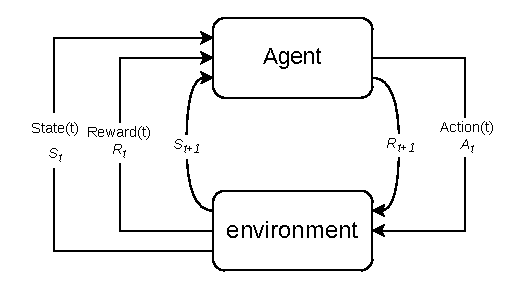
\includegraphics[width=\linewidth]{figures/DRL_process.pdf}
%	\caption{The framework of DRL.}
%	\label{fig:ppo_framework}
%\end{figure}

To enable the agent to perceive both the instantaneous dynamical state of the drive system and the current synchronization deviation, the full observation vector is defined as
\begin{equation}
	O_t
	=
	\frac{1}{c_o}
	\begin{bmatrix}
		x_1(t),x_2(t),x_3(t),
		e_1(t),e_2(t),e_3(t)
	\end{bmatrix}^{\mathrm T},
	\label{eq:observation_space}
\end{equation}
where $c_o=5.0$ is the fixed observation scaling used in implementation. The notation $c_o$ is used here to avoid confusion with the Gaussian noise intensity $\sigma$ used in the robustness experiments.

For PPO, the sampled Gaussian policy action during training, or its deterministic mean during evaluation, is clipped to $[-1,1]$ before deployment. Denoting this clipped action by $a_t$, it is mapped to the physical control input as
\begin{equation}
	u(t)=\kappa a_t,
	\label{eq:action_mapping}
\end{equation}
where $\kappa$ is the control scaling factor, and $\kappa=4$ is adopted in this paper.

Let $t_k=k\Delta t$ denote the control-update times. The applied input $u_k=\kappa a_k$ is held constant on $[t_k,t_{k+1})$. The environment then advances the drive and response and returns a reward based on the updated error:
\begin{equation}
	r_k
	=
	-0.1\|\mathbf{e}(t_{k+1})\|_1
	=
	-0.1\sum_{i=1}^{3}|e_i(t_{k+1})|.
	\label{eq:reward_function}
\end{equation}
Maximizing the discounted reward promotes small synchronization errors throughout the rollout. The reward contains no control-effort penalty; input magnitude is constrained by action clipping, and effort is measured separately during evaluation. The same error reward is retained in the reduced-observation and multi-input experiments to keep their learning objectives consistent.

PPO is selected for its direct Gaussian-policy parameterization and alternating rollout and minibatch-update implementation~\cite{schulman2017proximal}. These features fit the sampled scalar-feedback task. The SAC comparison in Table~\ref{tab:sac_comparison} assesses the sensitivity of the results to the learning algorithm.

To learn a control policy in the above continuous-action setting, this paper employs the PPO algorithm~\cite{schulman2017proximal}. PPO is an Actor--Critic method whose clipped surrogate moderates policy optimization through the action-probability ratio. This likelihood-ratio clipping is distinct from actuator clipping. The PPO objective function is written as
\begin{equation}
	L(\theta)
	=
	\hat{\mathbb{E}}_t
	\left[
	\min
	\left(
	\rho_t(\theta)\hat{A}_t,\,
	\mathrm{clip}
	\left(
	\rho_t(\theta),1-\epsilon,1+\epsilon
	\right)
	\hat{A}_t
	\right)
	\right],
	\label{eq:ppo_objective}
\end{equation}
where
\begin{equation}
	\rho_t(\theta)
	=
	\frac{\pi_\theta(\widetilde a_t|O_t)}
	{\pi_{\theta_{\mathrm{old}}}(\widetilde a_t|O_t)}.
	\label{eq:ppo_ratio}
\end{equation}
Here $\widetilde a_t$ is the unclipped Gaussian sample stored for the policy update, whereas $a_t=\operatorname{clip}(\widetilde a_t,-1,1)$ is applied to the environment. The ratio $\rho_t(\theta)$ compares the new and old action likelihoods, $\epsilon$ is the PPO clipping hyperparameter, and $\hat A_t$ is obtained using generalized advantage estimation (GAE). Optimization aims to reduce the discounted synchronization-error cost; attainment of its global minimum is not asserted.

\begin{figure*}[pos=!t,width=\textwidth]
\centering
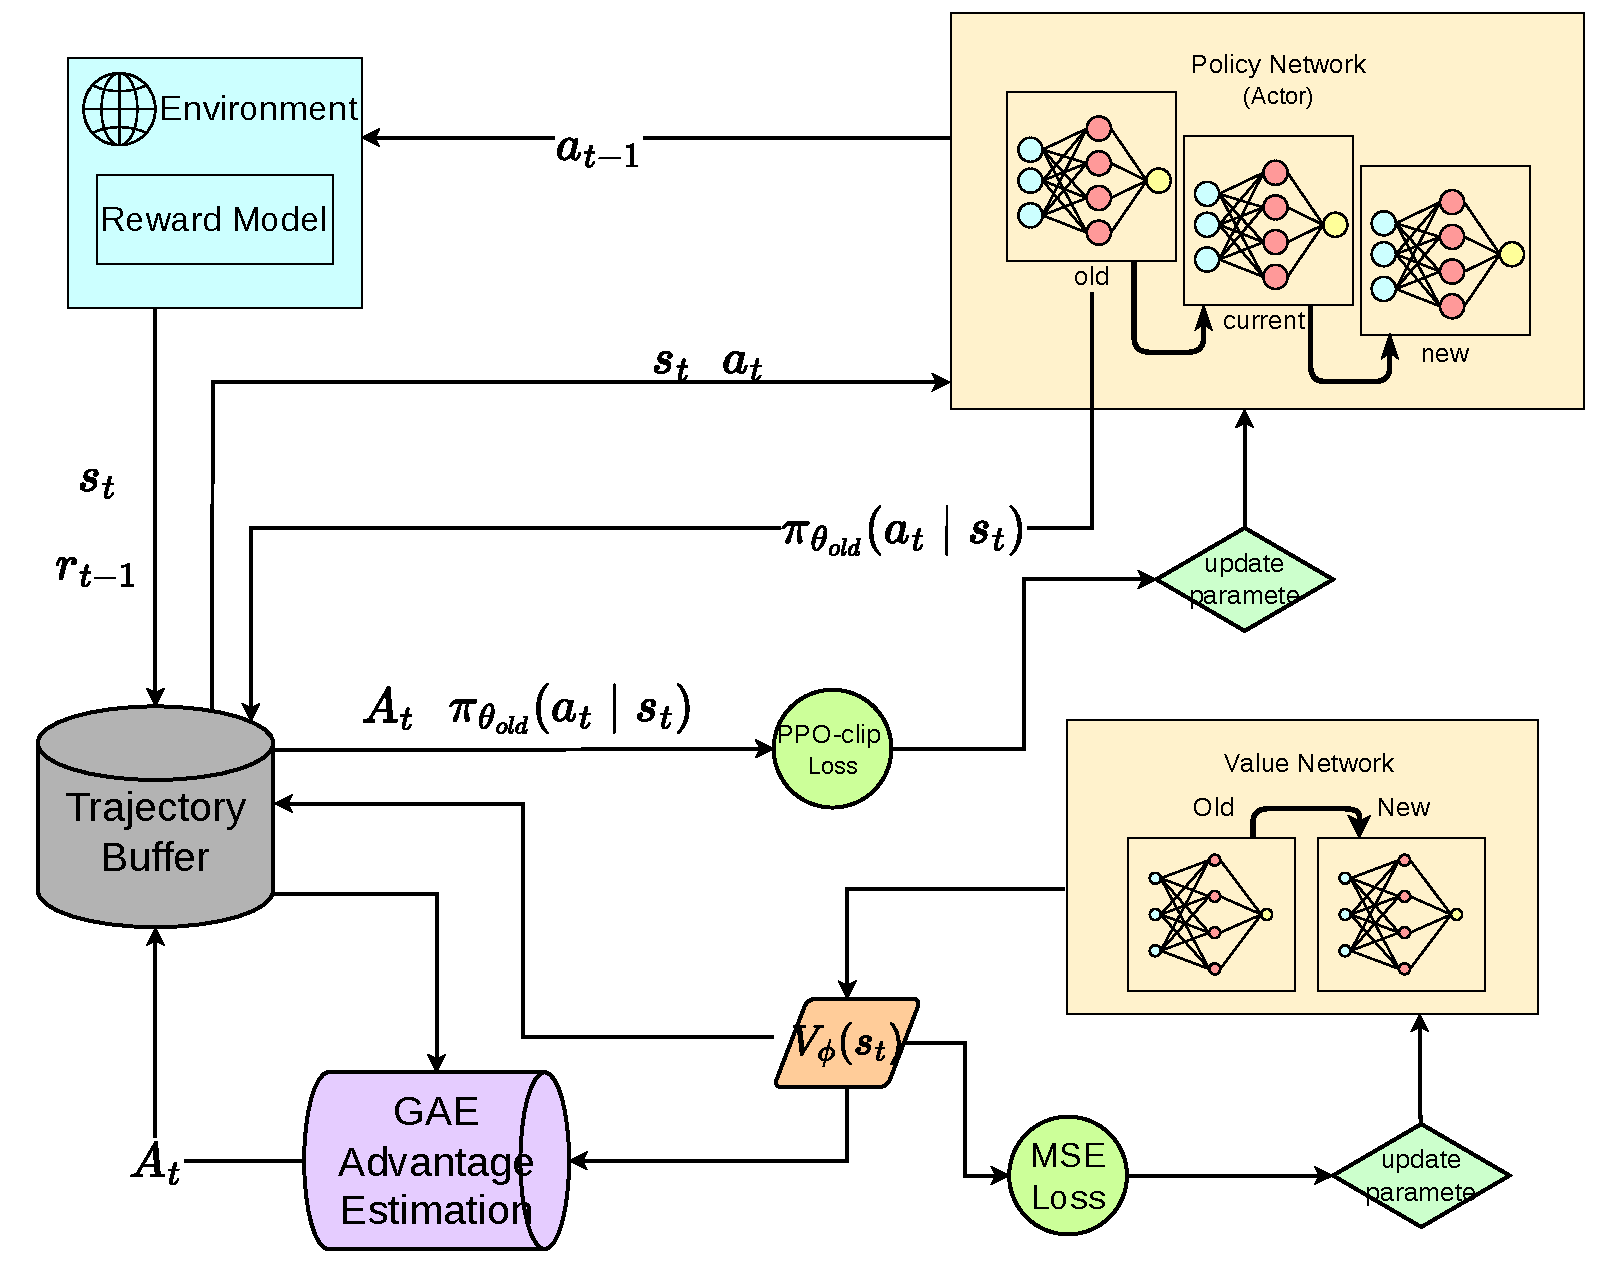
\includegraphics[width=\textwidth,height=0.78\textheight,keepaspectratio]{figures/ppo_process.pdf}
\caption{General training process of the PPO-based DRL framework.}
\label{fig:ppo_framework2}
\end{figure*}

As shown in Fig.~\ref{fig:ppo_framework2}, PPO follows an interaction--update training process. The agent first interacts with the environment using the current policy and stores the collected states, actions, rewards, and value estimates in a trajectory buffer. The advantage function is then estimated, typically using GAE, and the policy network is updated by maximizing a clipped surrogate objective. Meanwhile, the value network is trained by minimizing the mean squared error between the predicted and target state values. The clipped surrogate moderates likelihood-ratio changes during optimization; the deployed closed-loop behavior is assessed separately below.

The overall training procedure is summarized in Algorithm~\ref{alg:ppo_pinning}. In each iteration, trajectories are first collected by executing the current policy in the error-system environment. The collected data are then used to estimate the advantage function and update the policy network with the PPO clipped objective. The value network is updated by minimizing the squared value loss. After repeated interaction and optimization, the trained policy is used as the single-input pinning controller for the response system.

\subsection{Boundedness and Post-Training Local Numerical Assessment}
\label{subsec:boundedness_local_stability}

The trained policy is now treated as a fixed feedback law. Its assessment separates two questions: whether the controlled states remain bounded, and how nearby response trajectories evolve under the deployed controller. The first follows analytically from the dissipative Hopfield dynamics and bounded actuation. The second is examined numerically through the closed-loop control-step Jacobian, using the same sample-and-hold implementation as in deployment.

Because the normalized action satisfies $a_t\in[-1,1]$ and the physical action is defined by~\eqref{eq:action_mapping}, the deployed control input satisfies
\begin{equation}
	|u(t)|\leq \kappa,
	\qquad \kappa=4.
	\label{eq:bounded_control_input}
\end{equation}
Moreover, each single-node pinning vector has $\|B_i\|_2=1$.

\begin{proposition}[Boundedness of the controlled drive--response trajectories]
\label{prop:closed_loop_boundedness}
Consider the drive system~\eqref{eq:hopfield_simplified_vector} and response system~\eqref{eq:response_system}, where $W$ and $W_r$ are finite constant matrices and the control input is measurable and satisfies~\eqref{eq:bounded_control_input}. This includes the deployed piecewise-constant sample-and-hold input. For every finite initial condition, the corresponding trajectories are forward complete and uniformly ultimately bounded. In particular,
\begin{align}
	\limsup_{t\to\infty}\|\mathbf{x}(t)\|_2
	&\leq \sqrt{3}\|W\|_2,
	\label{eq:drive_ultimate_bound}\\
	\limsup_{t\to\infty}\|\mathbf{y}(t)\|_2
	&\leq \sqrt{3}\|W_r\|_2+\kappa.
	\label{eq:response_ultimate_bound}
\end{align}
\end{proposition}

\begin{proof}
Since $\|\tanh(\mathbf{z})\|_2\leq\sqrt{3}$ for every $\mathbf{z}\in\mathbb{R}^3$, the Cauchy--Schwarz inequality and the induced matrix norm give
\begin{align}
	D^+\|\mathbf{x}\|_2
	&\leq-\|\mathbf{x}\|_2+\sqrt{3}\|W\|_2, \notag\\
	D^+\|\mathbf{y}\|_2
	&\leq-\|\mathbf{y}\|_2+\sqrt{3}\|W_r\|_2+\|B_i\|_2|u(t)| \notag\\
	&\leq-\|\mathbf{y}\|_2+\sqrt{3}\|W_r\|_2+\kappa,
	\label{eq:state_norm_comparison}
\end{align}
where $D^+$ is the upper right Dini derivative, $\|B_i\|_2=1$, and~\eqref{eq:bounded_control_input} has been used. Applying the scalar comparison lemma to~\eqref{eq:state_norm_comparison} yields
\begin{equation}
	\|\mathbf{x}(t)\|_2
	\leq e^{-t}\|\mathbf{x}(0)\|_2
	+\sqrt{3}\|W\|_2(1-e^{-t}).
	\label{eq:drive_explicit_bound}
\end{equation}
\begin{equation}
	\|\mathbf{y}(t)\|_2
	\leq e^{-t}\|\mathbf{y}(0)\|_2
	+\left(\sqrt{3}\|W_r\|_2+\kappa\right)(1-e^{-t}).
	\label{eq:response_explicit_bound}
\end{equation}
Taking the upper limit as $t\to\infty$ gives~\eqref{eq:drive_ultimate_bound} and~\eqref{eq:response_ultimate_bound}. For a prescribed bounded measurable input, the vector field is globally Lipschitz in the state and has bounded forcing. The explicit bounds preclude finite escape; the sampled feedback can consequently be extended over successive control intervals for all future times.
\end{proof}

For the nominal matched case $W_r=W$, the matrix in~\eqref{eq:weight_matrix} has $\|W\|_2=8.9524$. Proposition~\ref{prop:closed_loop_boundedness} therefore gives the conservative bounds $\limsup_{t\to\infty}\|\mathbf{x}(t)\|_2\leq15.5059$ and $\limsup_{t\to\infty}\|\mathbf{y}(t)\|_2\leq19.5059$. These worst-case norm estimates establish non-divergence and provide conservative envelopes for the trajectories. In particular, boundedness of both trajectories alone does not imply that the synchronization error converges to zero.

The MCLE $\lambda_{\max}^{(c)}(B_i)$ in Section~\ref{subsec:local_node_selection} and the closed-loop exponent introduced below have different purposes. The former is a pre-training node-screening indicator derived from a locally linearized transverse model under the ideal pinning assumption and does not include the learned PPO policy. By contrast, the latter is evaluated after training from the actual deployed sample-and-hold closed-loop map. Consequently, their numerical values should not be directly compared or interpreted as equivalent stability measures.

The implementation uses a sample-and-hold controller: one action is evaluated every five RK4 substeps and is held constant over the control interval $\Delta t=0.05$. Accordingly, local behavior of the trained controller is assessed using the actual discrete control-step map
\begin{equation}
	\mathbf{x}_{k+1}=\Phi_x(\mathbf{x}_k),
	\qquad
	\mathbf{e}_{k+1}=G_i(\mathbf{x}_k,\mathbf{e}_k;\pi_{\theta,i}),
	\label{eq:sampled_closed_loop_map}
\end{equation}
where $G_i$ includes the deterministic mean action of the trained policy, action clipping, the physical scale $\kappa$, and the five RK4 substeps. The transverse Jacobian of the deployed map is
\begin{equation}
	M_{i,k}
	=
	\frac{\partial G_i}{\partial\mathbf{e}}
	(\mathbf{x}_k,\mathbf{e}_k;\pi_{\theta,i}).
	\label{eq:sampled_error_jacobian}
\end{equation}
The asymptotic largest conditional Lyapunov exponent is defined by
\begin{equation}
	\lambda_i^{\mathrm{cl}}
	=
	\limsup_{N\to\infty}
	\frac{1}{N\Delta t}
	\ln
	\left\|
	M_{i,N-1}M_{i,N-2}\cdots M_{i,0}
	\right\|_2.
	\label{eq:closed_loop_conditional_lyapunov}
\end{equation}
Automatic differentiation and QR renormalization are used to obtain a finite-time estimate $\widehat\lambda_i^{\mathrm{cl}}$ of the largest conditional Lyapunov exponent over the evaluation interval. A negative estimate indicates that small linearized perturbations to the response state decay on average along the tested trajectory, with the drive trajectory held fixed. This local decay does not imply zero synchronization error; therefore, the exponent and the synchronization residual are reported separately.

The numerical assessment was conducted for Nodes 2 and 3 using three independently trained policies for each node. Each policy was evaluated from ten initial conditions, giving 30 closed-loop trajectories per node and 60 trajectories in total. Each trajectory contained 2000 control intervals, and the first 100 intervals were discarded as a transient, leaving 95 time units for exponent accumulation. Table~\ref{tab:closed_loop_conditional_lyapunov} summarizes the largest conditional Lyapunov exponent and the post-transient synchronization residual. The reported mean error is obtained by first averaging $\|\mathbf{e}_k\|_2$ over the post-transient portion of each trajectory and then averaging over the 30 trajectories for the corresponding node.

No state guard was activated along these trajectories, so omitting that inactive operation from the differentiated map does not change the local derivative there. Action clipping is nonsmooth at its thresholds; the numerical derivatives describe behavior away from those thresholds.

\begin{center}
	\centering
	\small
	\captionof{table}{Finite-time conditional Lyapunov estimates for the deployed sample-and-hold PPO controllers.}
	\label{tab:closed_loop_conditional_lyapunov}
	\begin{tabular}{@{}cccc@{}}
		\toprule
		Node & $\widehat\lambda_i^{\mathrm{cl}}$ & Range & Mean $\|\mathbf{e}\|_2$ \\
		\midrule
		2 & $-1.117$ & $[-1.317,-0.872]$ & 0.0276 \\
		3 & $-0.581$ & $[-0.592,-0.557]$ & 0.0075 \\
		\bottomrule
	\end{tabular}
\end{center}

The finite-time estimate is negative for all 60 evaluated trajectories. A shorter check using 600 control intervals produced the same signs and similar aggregate values, supporting numerical consistency over the examined windows. Node 2 has a more negative mean estimate, whereas Node 3 has a smaller post-transient error. The two measurements describe complementary properties: local perturbation decay and residual synchronization error. In particular, the policy architecture does not impose $\pi_{\theta,i}(\mathbf{x},\mathbf{0})=0$. Thus, the synchronization manifold need not be invariant. Here ``practical synchronization'' describes the observed low-residual behavior over the evaluation window.


As a complementary multi-step check, a positive-definite metric $P$ was fitted once per policy using a separate nominal rollout. In the induced norm $\|\mathbf{v}\|_P=(\mathbf{v}^{\mathsf T}P\mathbf{v})^{1/2}$, the largest sampled gains of the ordered 40-step Jacobian products were 0.4882 and 0.5340 for Nodes 2 and 3, respectively; at 80 steps they were 0.0673 and 0.2802. These checks used 60 nominal trajectories of 2,000 control intervals, excluding the first 100 intervals. Forty control intervals correspond to two system time units. Direct paired-rollout checks with initial response perturbations up to 0.05 along signed coordinate directions also showed contraction at these horizons.

\begin{algorithm}[t]
	\caption{PPO-based Single-Input Pinning Control for the Error System}
	\label{alg:ppo_pinning}
	\begin{algorithmic}[1]
		\Require Error-system environment $\mathcal{E}$; policy network $\pi_{\theta}$; value network $V_{\phi}$; learning rate $\eta$; clipping parameter $\epsilon$; discount factor $\gamma$; GAE parameter $\lambda$.
		\Ensure Optimized policy parameters $\theta$.
		
		\State Initialize policy parameters $\theta_0$ and value-function parameters $\phi_0$.
		\State Initialize the drive--response system and obtain the initial observation $O_0$.
		\State Define a trajectory buffer $\Gamma$ to store observations, actions, rewards, and value estimates.
		
		\For{$k = 0,1,2,\ldots,K-1$}
		\State Collect trajectories $\Gamma_k$ by executing the current policy $\pi_{\theta_k}$ in the environment.
		\For{each time step $t$ in $\Gamma_k$}
		\State Sample $\widetilde a_t \sim \pi_{\theta_k}(\cdot|O_t)$; set $a_t=\operatorname{clip}(\widetilde a_t,-1,1)$.
		\State Store the unclipped sample for the policy update; apply $u(t)=\kappa a_t$.
		\State Apply $u(t)$ to the response system and observe reward $r_t$ and next observation $O_{t+1}$.
		\EndFor
		
		\State Compute advantage estimates $\hat{A}_t$ using generalized advantage estimation.
		\State Update policy parameters by maximizing the PPO clipped objective:
		\Statex
		\[
		\begin{aligned}
			\theta_{k+1}=\arg\max_{\theta}\hat{\mathbb{E}}_t\Big[
			\min\big(&\rho_t(\theta)\hat{A}_t,\\
			&\mathrm{clip}(\rho_t(\theta),1-\epsilon,1+\epsilon)\hat{A}_t\big)
			\Big].
		\end{aligned}
		\]
		\Statex
		where
		\[
		\rho_t(\theta)
		=\frac{\pi_{\theta}(\widetilde a_t|O_t)}
		{\pi_{\theta_k}(\widetilde a_t|O_t)}.
		\]
		
		\State Update value-function parameters by minimizing the squared value loss:
		\Statex
		\[
		\phi_{k+1}
		=
		\arg\min_{\phi}
		\hat{\mathbb{E}}_t
		\left[
		\left(
		V_{\phi}(O_t)-\hat{R}_t
		\right)^2
		\right].
		\]
		\EndFor
		
		\State \Return trained policy $\pi_{\theta}$.
	\end{algorithmic}
\end{algorithm}

Together, the one-step and multi-step assessments explain how local perturbations can decay over finite windows even when individual steps amplify them. State boundedness supplies the analytical foundation, while trajectory sensitivity and measured residuals describe distinct aspects of the trained feedback behavior. The numerical assessment is restricted to the sampled trajectories rather than a certified neighborhood-wide error bound. Building on this distinction, the following experiments compare synchronization accuracy, transient recovery, and control effort across configurations and operating conditions. 

\section{Experimental Results and Analysis}
\label{sec:experiments}

The experiments address three questions: how actuator location affects PPO performance and observation demand; what changes when additional actuators become available; and how the trained PPO policies compare with alternative controllers under parameter mismatch~\cite{kobiolka2025reducedorder}, impulse disturbances, and process noise. The comparisons report synchronization error and applied control effort under the stated shared test conditions.

\subsection{Experimental Setup and Evaluation Metrics}
\label{subsec:experimental_setup}



The programs were implemented in Python using Stable Baselines3. The workstation is equipped with an NVIDIA RTX 5070Ti graphics processing unit (GPU); the policy training scripts considered here use the central processing unit (CPU). PPO used a nominal training budget of $4\times10^5$ environment transitions, with four parallel environments and 512 steps per environment in each rollout.

During environment interaction, the continuous-time system dynamics were integrated using the RK4 method. The basic integration step size was set to $0.01$ time units. To improve numerical stability, five RK4 substeps were performed within each control step. Therefore, each control update corresponded to an effective time interval of $0.05$ time units. The maximum magnitude of the physical control input was constrained to 4 units.

The implementation also contains a numerical state guard at $[-10,10]$ after RK4 substeps and disturbance updates. No guard activation was detected in the 2,940 reevaluated episodes covering the traditional baselines, matched-budget SAC comparison, and actuator-count ablation; the reported trajectories in these comparisons therefore evolve without state truncation.

At initialization, the initial states of both the drive system and the response system, denoted by $\mathbf{x}(0)$ and $\mathbf{y}(0)$, were sampled from the uniform distribution $[-1.0,1.0]$. This common distribution provides varied initial synchronization errors and is held fixed across the compared methods. The reported results are conditional on this initialization range.

For the reinforcement learning configuration, both the policy network and the value network were represented by multilayer perceptrons (MLPs). The Adam optimizer was adopted with a learning rate of $3\times 10^{-4}$, so as to balance exploration efficiency and policy-update stability.

Three traditional controllers are included to provide references of increasing model dependence. First, the original fixed-gain feedback baseline~\cite{yassen2005controlling} is retained without retuning:

\begin{equation}
	u(t)=
	\begin{cases}
		-4, & -k e_i(t)<-4,\\
		-k e_i(t), & -4\leq -k e_i(t)\leq 4,\\
		4, & -k e_i(t)>4,
	\end{cases}
	\label{eq:linear_feedback_baseline}
\end{equation}
where $e_i(t)$ denotes the synchronization error at the controlled node $i$. This baseline represents a simple local-error controller rather than an optimally tuned linear design. The previously selected gain $k=8.0$ is used throughout all reported experiments.

Second, a continuous-time LQR baseline is obtained from the error model linearized at the origin in Section~\ref{sec:ppo_pinning_method}. With $Q=I_3$ and $R=1$, its saturated control law is
\begin{equation}
	u_{\mathrm{LQR},i}(t)=\operatorname{sat}_{4}\!\left[-K_i\mathbf e(t)\right],
	\label{eq:lqr_baseline}
\end{equation}
where $K_i=R^{-1}B_i^{\mathrm T}P_i$ and $P_i$ is the stabilizing solution of the continuous algebraic Riccati equation associated with $(A,B_i)$. The resulting gains are
\[
\begin{aligned}
K_2&=(-0.116727,\ 3.871191,\ -5.502161),\\
K_3&=(-0.171698,\ -2.085641,\ 3.850986).
\end{aligned}
\]
Unlike fixed-gain feedback, LQR uses all error components and the nominal local model. The principal error--effort assessment includes the design with $R=0.01$ selected using separate validation initial conditions in Table~\ref{tab:lqr_weight_sensitivity}. The original $R=1$ design is retained in the scenario curves as a reference for weight sensitivity, not as the strongest LQR comparator. The resulting feedback is evaluated on the nonlinear system with actuator saturation.

Third, a boundary-layer SMC is included as a nonlinear model-based baseline~\cite{feki2009sliding,su2021fixed}. Define
\begin{equation}
	\mathbf g_0(\mathbf x,\mathbf y)=-\mathbf e+W\left[\tanh(\mathbf y)-\tanh(\mathbf x)\right],
	\label{eq:nominal_error_drift}
\end{equation}
and select $c_i^{\mathrm T}=K_i/(K_iB_i)$ so that $c_i^{\mathrm T}B_i=1$. The sliding variable and control law are
\begin{equation}
	s_i=c_i^{\mathrm T}\mathbf e,\qquad
	u_{\mathrm{SMC},i}=\operatorname{sat}_{4}\!\left[-c_i^{\mathrm T}\mathbf g_0-k_s\operatorname{sat}\!\left(\frac{s_i}{\phi}\right)\right],
	\label{eq:smc_baseline}
\end{equation}
where $\operatorname{sat}(z)=\max(-1,\min(1,z))$, $k_s=16$, and $\phi=0.5$. These parameters minimize the recorded validation score over $k_s\in\{4,8,12,16\}$ and $\phi\in\{0.2,0.5,1,2\}$, using ten validation initial conditions separate from the test seeds. Validation includes nominal, mismatch ($\eta=1$), and impulse scenarios; the score averages their mean absolute errors normalized by 0.1, 0.15, and 0.45, respectively. The selected parameters are kept unchanged during testing. Thus, although its compensation term uses the nominal model, SMC parameter selection has access to non-ideal validation scenarios. The saturated, sampled implementation is evaluated empirically; the continuous-time ideal sliding condition is not asserted to hold when the actuator saturates.

All four methods use the same RK4 solver, control-update interval, initial-state distribution, testing horizon (400 updates, or 20 time units), and actuator bound $|u|\leq4$. The PPO results aggregate three independently trained policies, each evaluated on 20 common test seeds ; each deterministic traditional controller is evaluated on the same 20 test seeds. For each scenario, the initial conditions and exogenous random realizations are shared across controllers. In the existing environment, drawing a mismatch matrix consumes random numbers before initialization; hence a fixed seed does not imply identical initial states between $\eta=0$ and $\eta>0$. Comparisons between controllers are paired within each scenario.

PPO is trained only on the nominal system. LQR uses $\mathbf e$ and the nominal local model, while SMC additionally uses $\mathbf x$ and $\mathbf y$ for nonlinear compensation. PPO receives $(\mathbf x,\mathbf e)/5$ without evaluating an analytical model during deployment; its training simulator nevertheless uses the nominal dynamics. Fixed-gain feedback uses only $e_i$. Consequently, these are comparisons under matched actuation constraints, not identical information or design objectives. In particular, the PPO reward penalizes synchronization error but not control energy, whereas LQR explicitly penalizes both. Lower error at higher energy is therefore interpreted as a performance--effort tradeoff, not evidence of superior energy efficiency.

To evaluate the synchronization performance of different control methods, several metrics are introduced from the perspectives of overall synchronization accuracy, steady-state error, transient recovery capability, and control effort. Let $T=400$ denote the number of control updates and $N=3$ the system dimension. For the baseline and ablation comparisons, errors are recorded at the $T+1$ sampling instants including initialization. The synchronization error vector is
\begin{equation}
	\mathbf{e}(t)=\mathbf{y}(t)-\mathbf{x}(t)
	=
	[e_1(t),e_2(t),\ldots,e_N(t)]^{\mathrm T}.
	\label{eq:error_vector_metrics}
\end{equation}

The mean absolute error (MAE) is used to measure the average synchronization deviation over the whole testing interval:
\begin{equation}
	\mathrm{MAE}
	=
	\frac{1}{(T+1)N}
	\sum_{t=0}^{T}
	\sum_{i=1}^{N}
	|e_i(t)|.
	\label{eq:mae}
\end{equation}
MAE provides an intuitive measure of the overall error level by assigning equal weights to different time steps and state components.

The root mean square error (RMSE) is used to characterize the overall error level while being more sensitive to large deviations:
\begin{equation}
	\mathrm{RMSE}
	=
	\sqrt{
		\frac{1}{(T+1)N}
		\sum_{t=0}^{T}
		\sum_{i=1}^{N}
		e_i^2(t)
	}.
	\label{eq:rmse}
\end{equation}
Compared with MAE, RMSE is more sensitive to transient large errors and is therefore useful for evaluating error fluctuations under parameter mismatch and impulse disturbance.

The final L1 error is used to measure the synchronization accuracy at the end of testing:
\begin{equation}
	E_f=\|\mathbf{e}(T)\|_1
	=
	\sum_{i=1}^{N}|e_i(T)|.
	\label{eq:final_l1_error}
\end{equation}
This metric reflects how closely the response system approaches the drive system at the final testing instant.

In the impulse disturbance experiment, the maximum post-pulse error is used to describe the largest error overshoot after the disturbance is injected:
\begin{equation}
	M_p=\max_{t\geq t_p}\|\mathbf{e}(t)\|_1,
	\label{eq:max_post_pulse_error}
\end{equation}
where $t_p$ denotes the impulse injection step. The imposed state jump largely determines the immediate peak, so $M_p$ alone is not interpreted as a controller-dependent recovery measure.

The post-pulse mean error is defined as the average global synchronization error from the impulse injection time to the end of testing:
\begin{equation}
	E_{\mathrm{post}}
	=
	\frac{1}{T-t_p+1}
	\sum_{t=t_p}^{T}
	\|\mathbf{e}(t)\|_1,
	\label{eq:post_pulse_mean_error}
\end{equation}
where $t_p$ is the impulse injection time and $T$ is the final testing step.

The control energy is used to measure the cumulative control effort over the testing process, summing over all $m$ active input channels:
\begin{equation}
	E_u=
	\sum_{t=1}^{T}
	\sum_{j=1}^{m}u_j^2(t)\Delta t,
	\label{eq:control_energy}
\end{equation}
where $\Delta t=0.05$ is the effective control update interval and $u_j(t)$ is the applied, saturated input during update $t$. The single-input comparisons have $m=1$. The steady L1 error averages $\|\mathbf e(t)\|_1$ over samples $t=320,\ldots,400$ (the final four time units), and differs from the terminal error $E_f$. Reported means first average the test initial conditions for each policy and then average policy seeds; the deterministic baselines have only the first level. Repeated initial conditions for the same trained policy are not treated as independent training replications.

In summary, MAE and RMSE are used to evaluate the overall synchronization performance, Final L1 Error is used to describe the terminal synchronization accuracy, $M_p$ and $E_{\mathrm{post}}$ are used to characterize transient recovery capability under impulse disturbance, and $E_u$ is used to assess the control cost.

\subsection{Effects of Control Location, Observation Variables, and Input Count}
\label{subsec:node_selection_observation}

We first fix the learning setup and vary the actuator location to test the screening preference from Section~\ref{sec:ppo_pinning_method}. The single control input is applied separately to Nodes 1, 2, and 3. The resulting comparison provides the starting point for asking how much feedback information each location needs within the same training budget.

Fig.~\ref{fig:pinning_node_comparison} shows faster error decay and a smaller residual at Node 3 than at Node 2, while Node 1 gives the weakest learned performance under the common budget. These results motivate examining Nodes 2 and 3 more closely: both support low-residual synchronization with full observations, but their response to restricted feedback may differ.

\begin{figure*}[pos=!t,width=\textwidth]
	\centering
	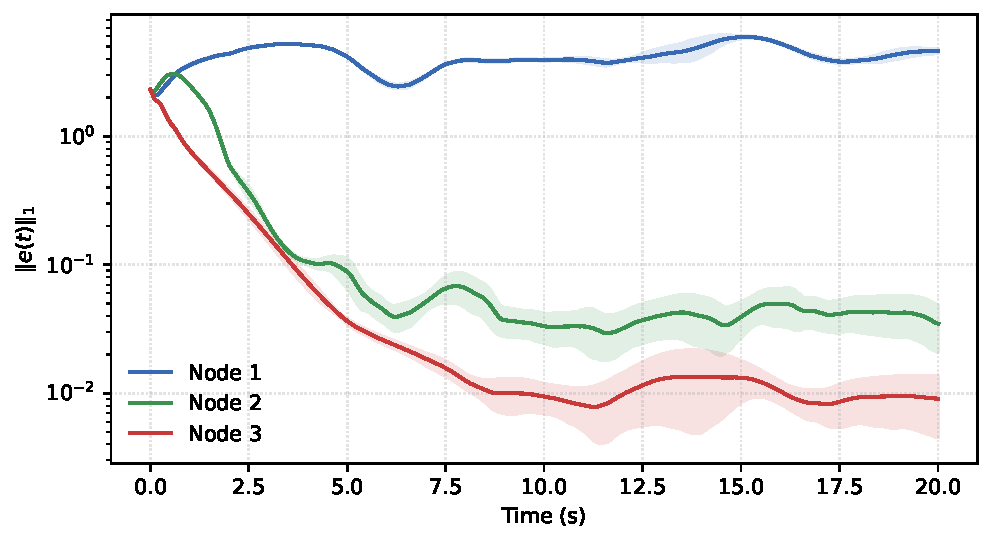
\includegraphics[width=0.88\textwidth]{figures/node_selection_audited.pdf}
	\caption{Synchronization error under different pinning nodes. Curves show training-run averages; shading indicates one sample standard deviation (SD) across runs.}
	\label{fig:pinning_node_comparison}
\end{figure*}

To avoid relying only on a single error curve for qualitative judgment, MAE, RMSE, and Final L1 Error are further used to quantitatively compare the synchronization performance under different pinning nodes. The results in Table~\ref{tab:pinning_node_metrics} further confirm the above observation. In terms of both average error and terminal error, Node 3 achieves the best overall synchronization performance. This result is generally consistent with the local auxiliary indicators in Table~\ref{tab:local_node_metrics}, including the $\lambda_{\max}^{(c)}$, $J_R$, $\|K_i\|$, and $V_i$. Thus the favorable Node 3 screening result is reflected in the tested policies. Agreement within this network supports the use of the indicators as local diagnostics; it does not establish a general predictor of PPO performance.

\begin{table}[pos=htbp,width=\linewidth]
	\centering
	\caption{Synchronization performance under different pinning nodes. MAE and RMSE are computed from the three error components.}
	\label{tab:pinning_node_metrics}
	\begin{tabular}{@{}lccc@{}}
		\toprule
		Node & MAE & RMSE & \makecell{Final L1\\Error} $E_f$\\
		\midrule
		Node 1 & 1.3937 & 1.6342 & 4.6052 \\
		Node 2 & 0.0930 & 0.2863 & 0.0347 \\
		Node 3 & 0.0431 & 0.1434 & 0.0091 \\
		\bottomrule
	\end{tabular}
\end{table}

The component-level surfaces in Fig.~\ref{fig:node_error_comparison} complement the aggregate error metrics. They show decay toward low error at Nodes 3 and 2 and persistent fluctuations at Node 1 across the displayed initial conditions. Surface height represents signed component error, with time and test index on the other axes. Since test index is categorical, interpolation between trajectories serves only to visualize their differences; quantitative comparisons use Table~\ref{tab:pinning_node_metrics}.

\begin{figure*}[pos=!t,width=\textwidth]
	\centering
\setlength{\tabcolsep}{3pt}
\begin{tabular}{@{}ccc@{}}
Node 3 & Node 2 & Node 1\\
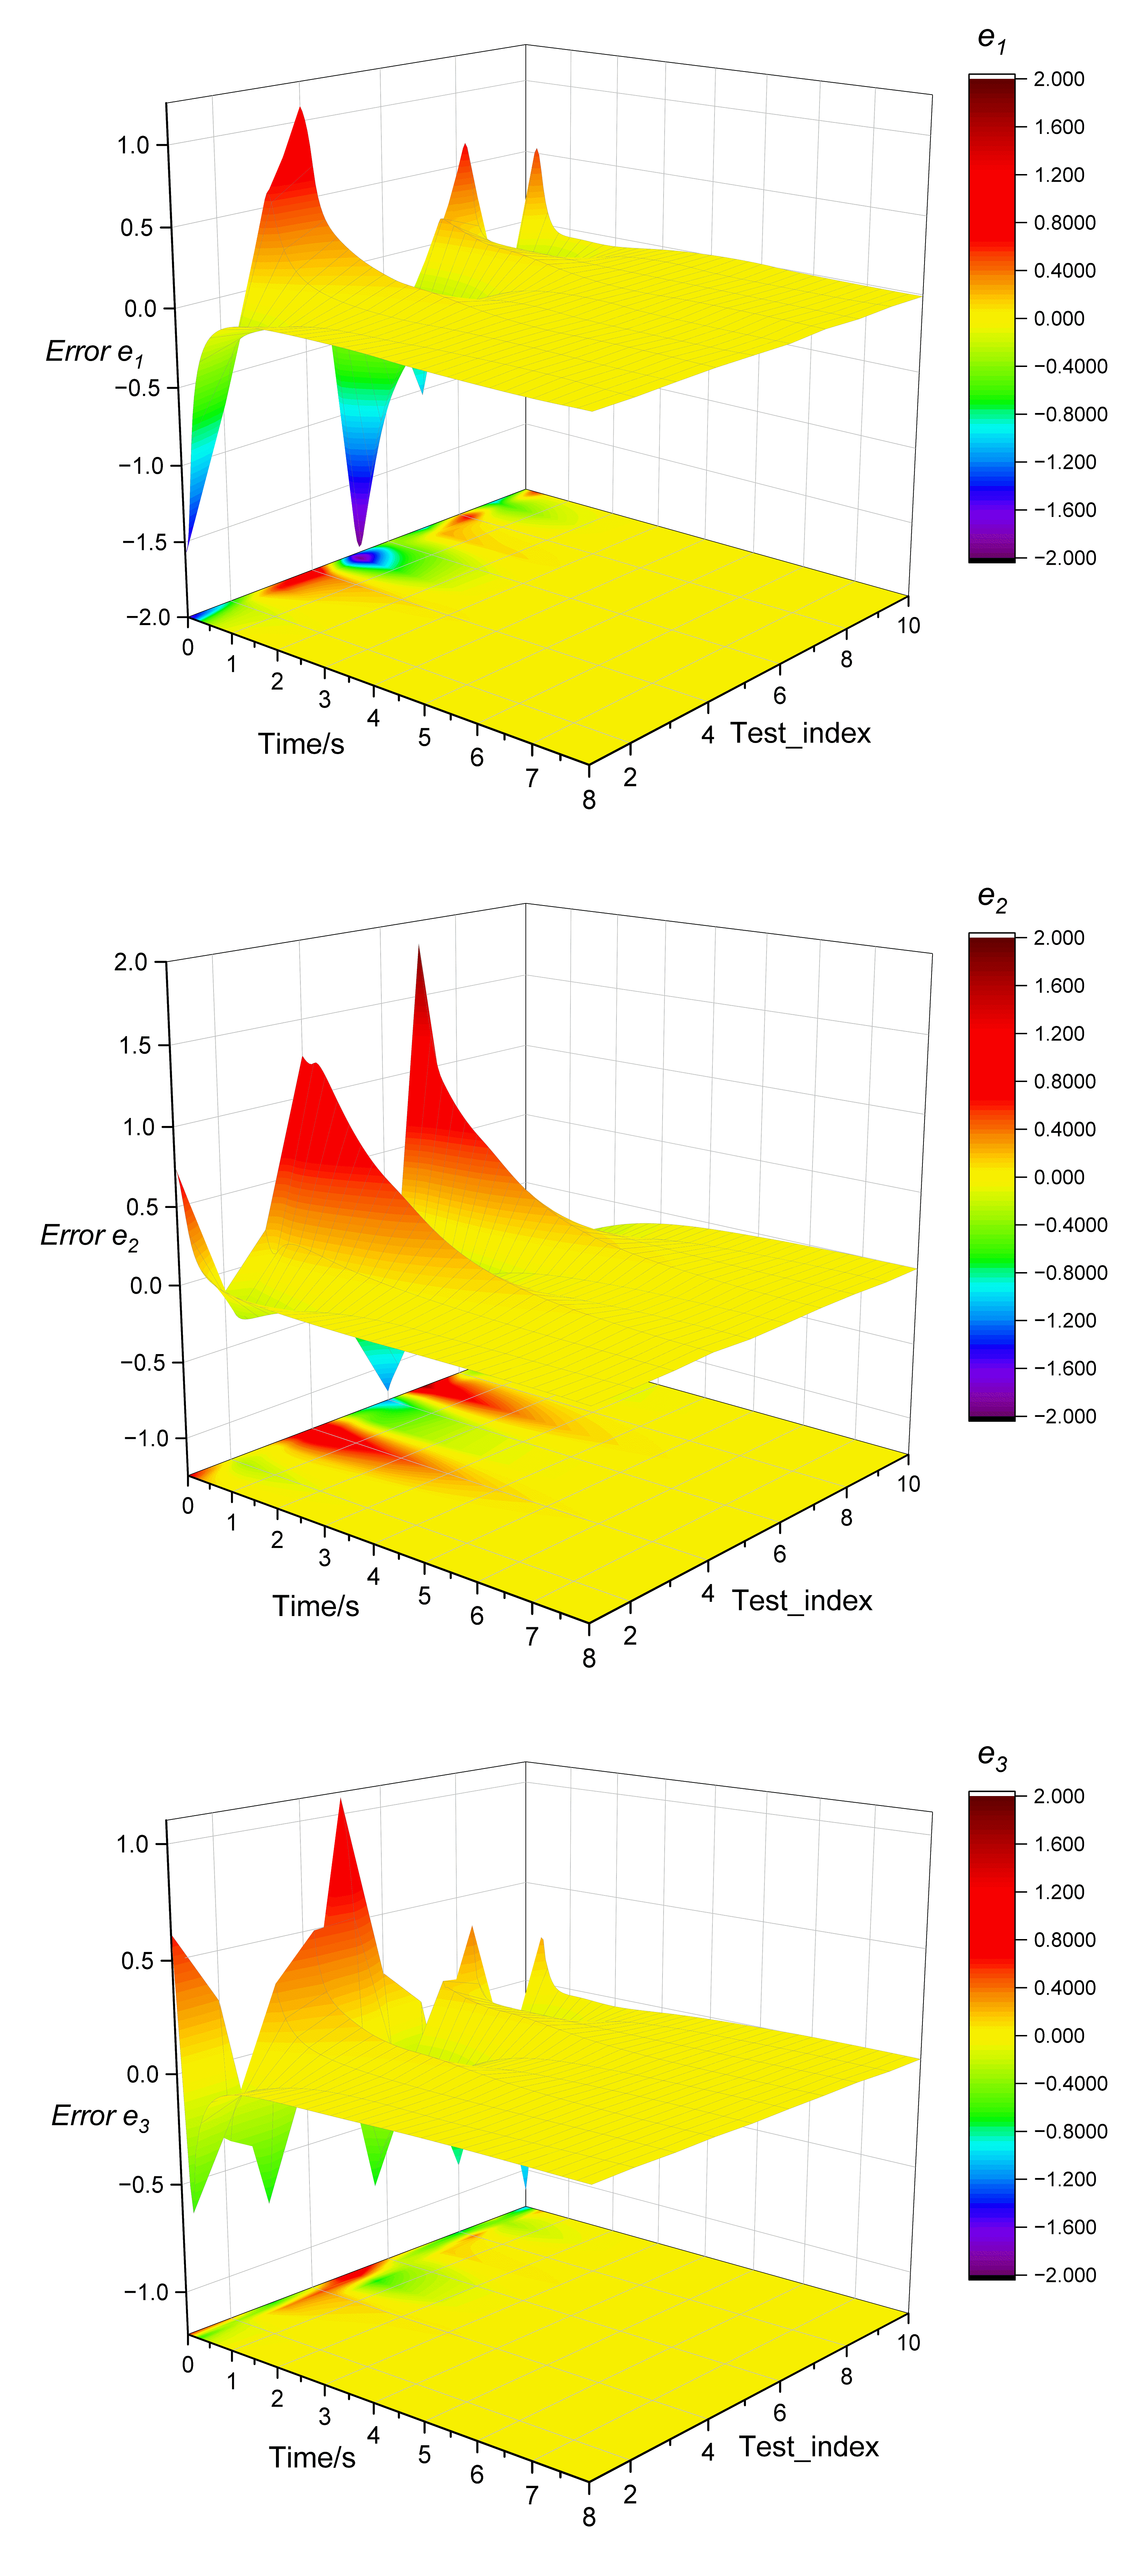
\includegraphics[width=0.32\textwidth]{figures/node3_error.png} &
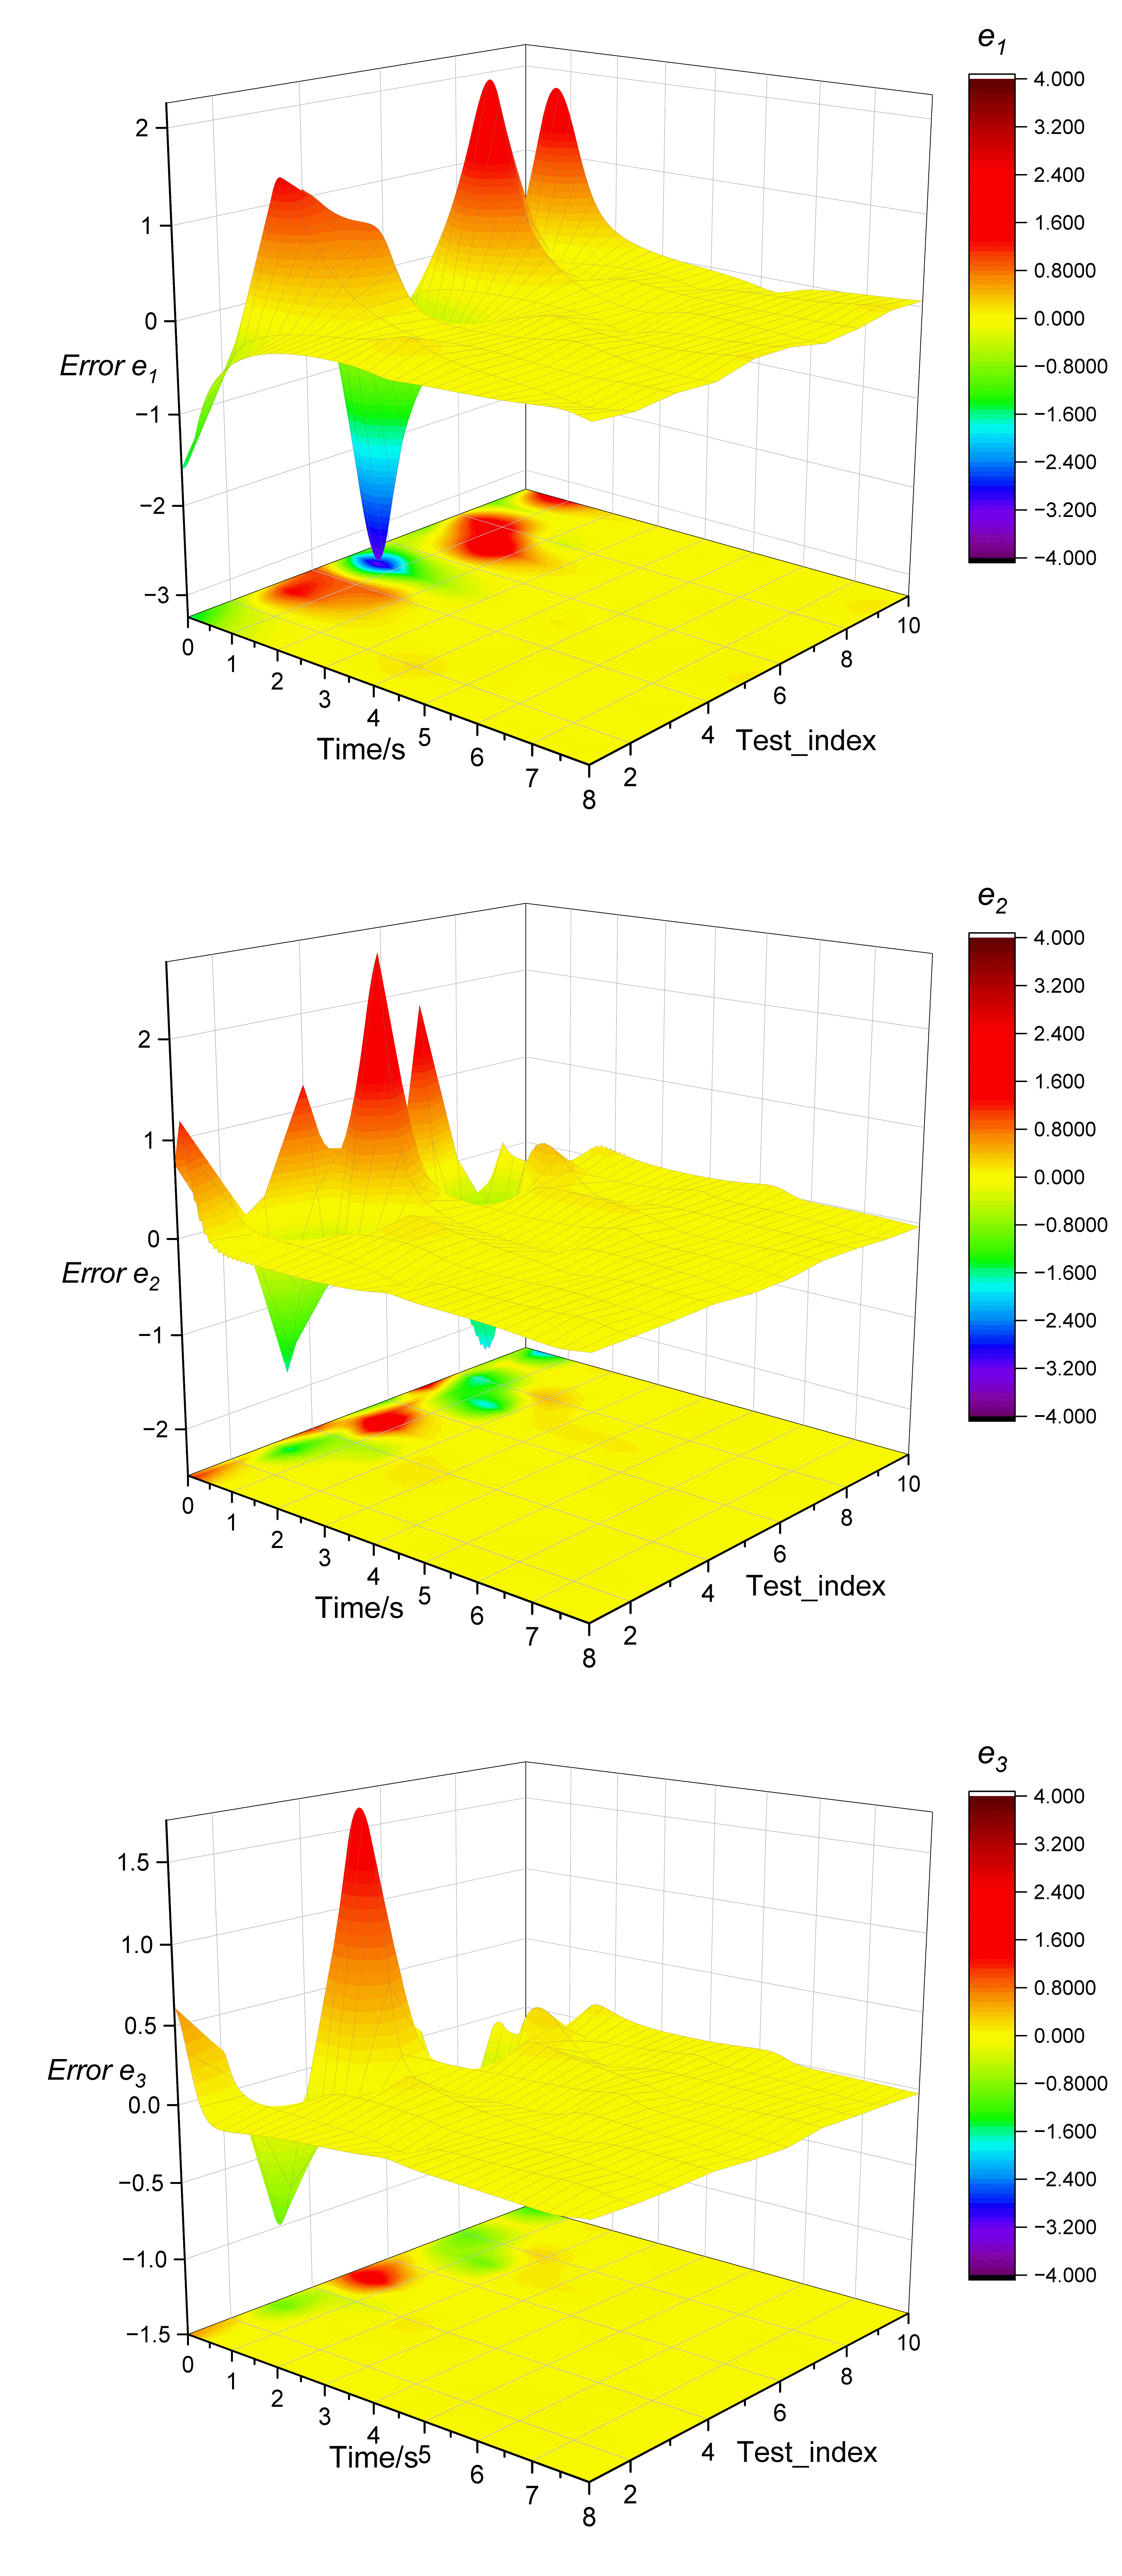
\includegraphics[width=0.32\textwidth]{figures/node2_error.png} &
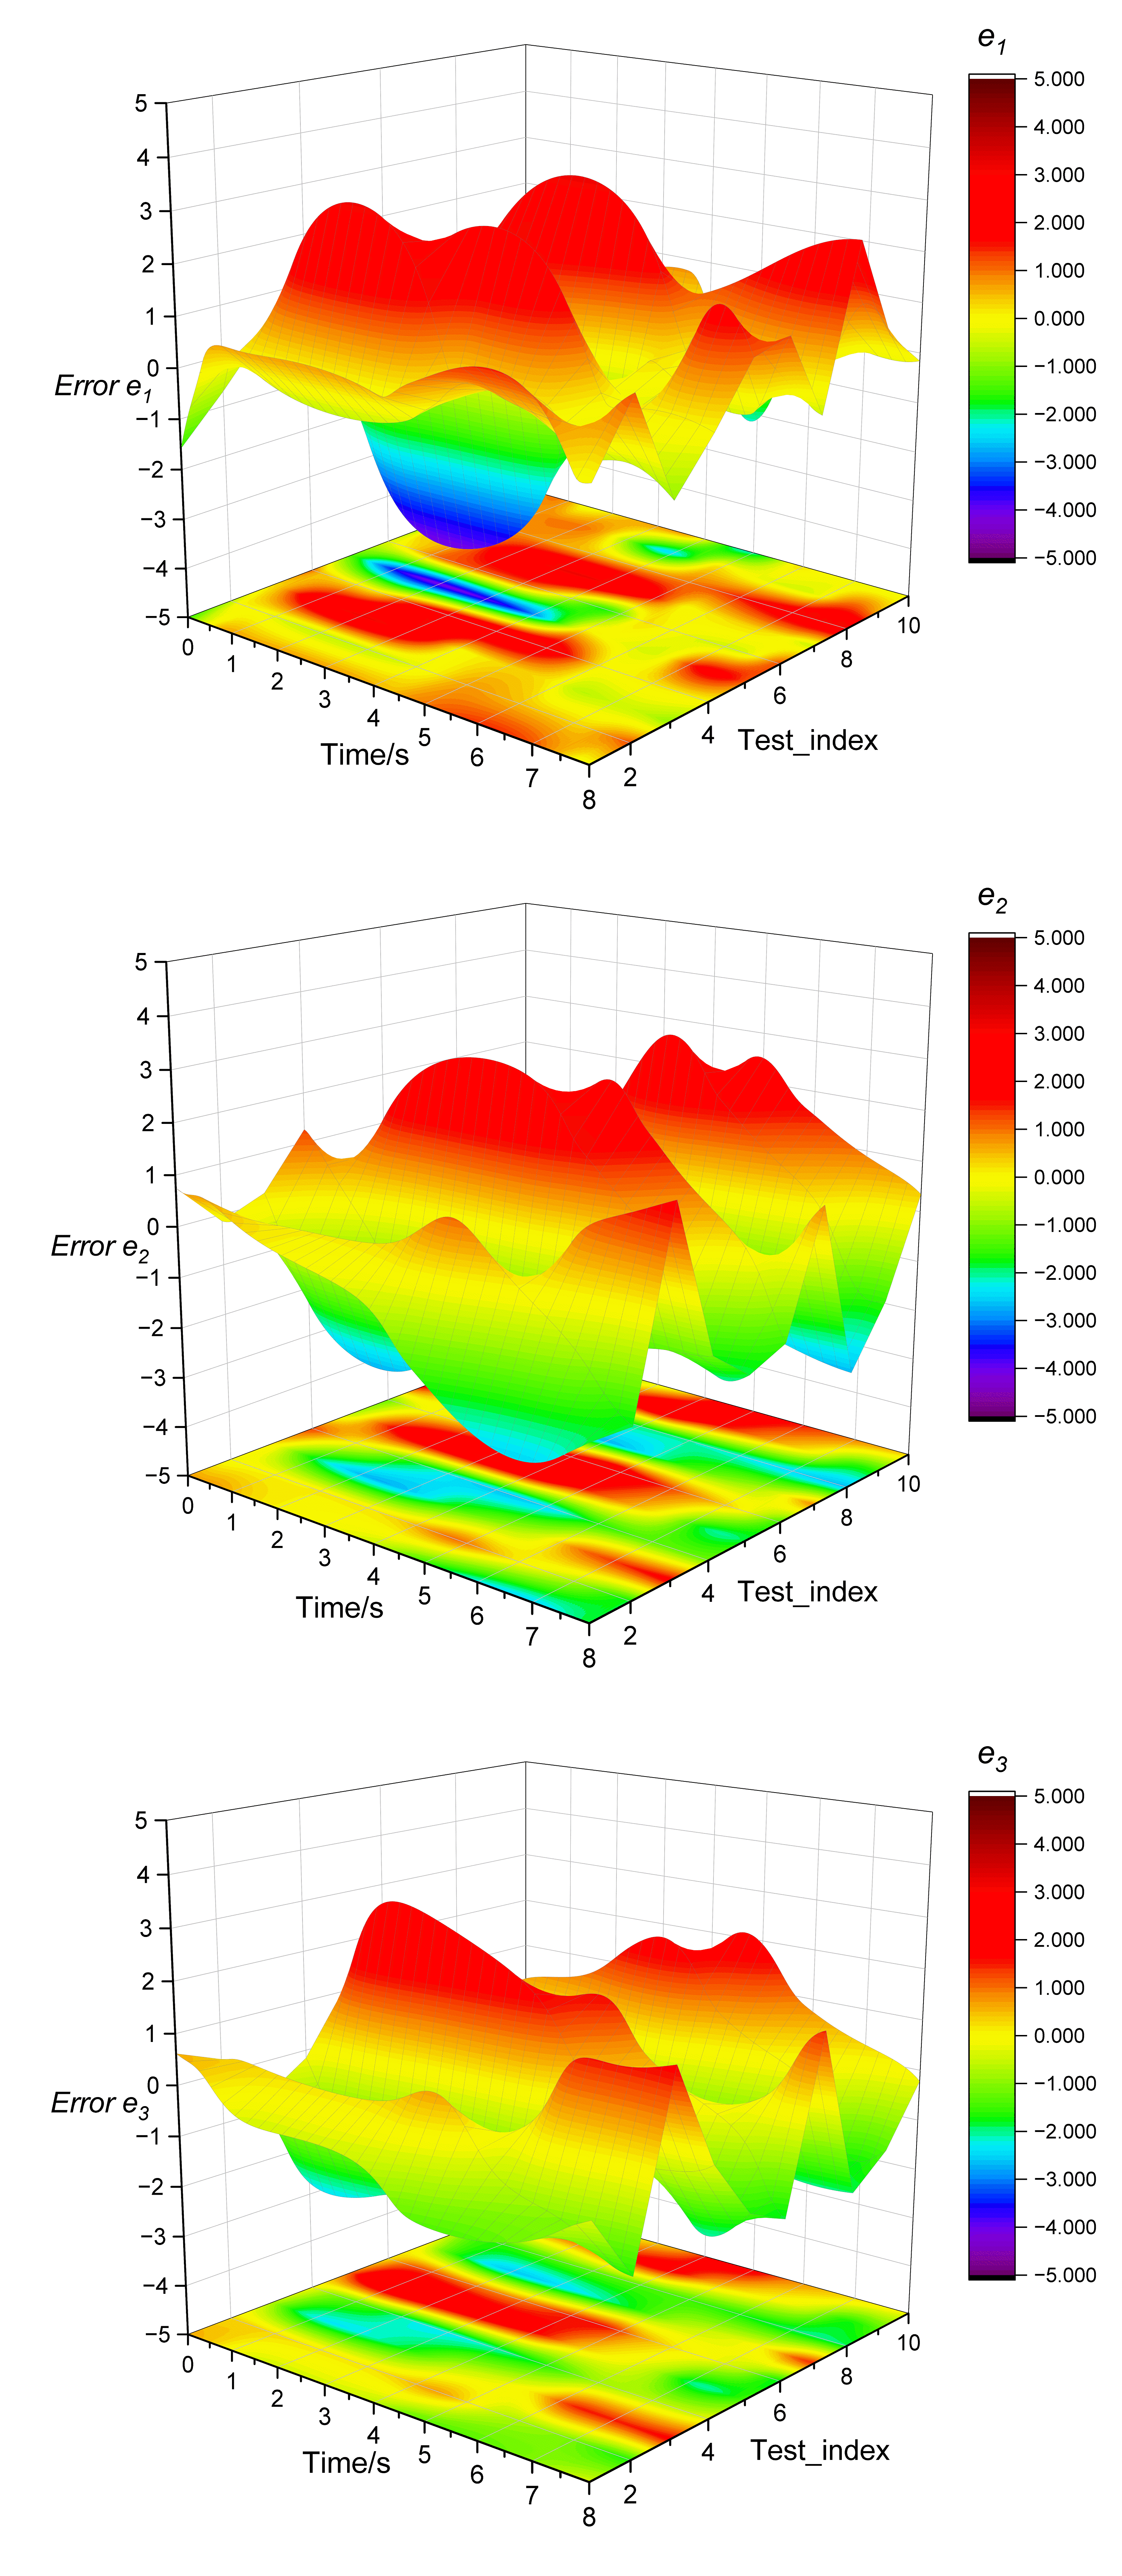
\includegraphics[width=0.32\textwidth]{figures/node1_error.png}
\end{tabular}
\caption{Three-dimensional synchronization-error surfaces for multiple initial conditions. Columns correspond to actuation at Nodes 3, 2, and 1; within each column, panels show $e_1$, $e_2$, and $e_3$ from top to bottom. Height and color represent signed error. Axis and color ranges differ between panels; quantitative comparisons across nodes should use the indicated scales.}
	\label{fig:node_error_comparison}
\end{figure*}

Node 3 is retained as the favorable candidate and Node 2 as a contrasting, more challenging learned-control channel. Both are evaluated in the subsequent robustness and algorithm comparisons, allowing actuator placement to be considered alongside controller choice.


Partial observability is next considered to examine how the information demand of the learned policy depends on the selected pinning node~\cite{weissenbacher2025reinforcement}. Within each node, the actuation structure and training procedure are retained while a separate policy is trained for each observation configuration. Thus, this comparison concerns the performance attainable by the trained configurations, not the effect of removing measurements from one unchanged policy.

For Node 3, the full-observation policy has access to all drive states and synchronization errors. The four-dimensional and two-dimensional observations are
\begin{equation}
	O_{4D}=\{x_1,x_3,e_1,e_3\},
	\label{eq:obs_4d}
\end{equation}
and
\begin{equation}
	O_{2D}=\{x_3,e_3\},
	\label{eq:obs_2d}
\end{equation}
respectively. For Node 2, the corresponding observations are $\{x_1,x_2,e_1,e_2\}$ and $\{x_2,e_2\}$.

The four-dimensional observation contains the drive states and synchronization errors of Node 1 and the controlled node: $\{x_1,x_2,e_1,e_2\}$ for control at Node 2 and $\{x_1,x_3,e_1,e_3\}$ for control at Node 3. Observing Node 1 does not add a control input there; actuation remains restricted to the selected node. These subsets provide an intermediate comparison between full observation and observation of the controlled node alone. Only the policy inputs are reduced: the simulator still computes the training reward from all three error components in~\eqref{eq:reward_function}. The policy uses the current observation without a history of past measurements, so the reduced input need not provide a complete Markov state.

\begin{figure*}[pos=!t,width=\textwidth]
	\centering
	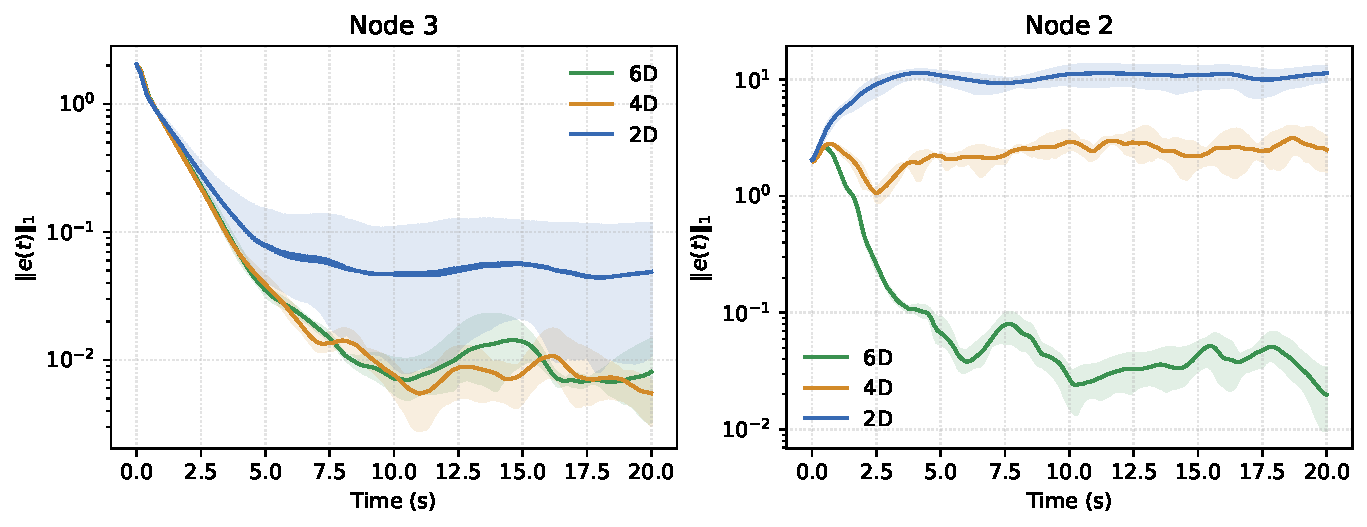
\includegraphics[width=\textwidth]{figures/observation_comparison_audited.pdf}

	\caption{Comparison of L1 synchronization error under different observation configurations. Curves average three training-seed means, with ten common archived test initial conditions per seed; shading spans the minimum and maximum of the three seed means. This archived observation experiment uses fewer test initial conditions than the baseline and actuator-count comparisons.}
	\label{fig:partial_observation_comparison}
\end{figure*}

Fig.~\ref{fig:partial_observation_comparison} and Table~\ref{tab:partial_observation} show similar later-stage errors for the Node 3 full- and four-dimensional policies. The tested two-dimensional policies have higher MAE and terminal error. This difference reflects both the available measurements and the policies learned from them. To compare the increase in error within each node, normalize MAE by that node's six-dimensional value. The four- and two-dimensional penalties are approximately 10.5 and 43.7 at Node 2, versus 1.0 and 1.3 at Node 3. These descriptive ratios, calculated from the common-seed means in Table~\ref{tab:partial_observation}, quantify the actuator-dependent consequence of reducing the selected policy inputs.

\begin{table}[pos=h,width=\linewidth]
	\centering
	\setlength{\tabcolsep}{3pt}
	\renewcommand{\arraystretch}{1.12}
	\caption{Synchronization performance under different observation settings, restricted to the same three training seeds and ten common test initial conditions. MAE is obtained by dividing the recorded time-averaged L1 error by $N=3$. Observation components are specified in Eqs.~\ref{eq:obs_4d}--\ref{eq:obs_2d}.}
	\label{tab:partial_observation}
	\begin{tabular}{@{}lcc@{}}
		\toprule
		Observation Setting & MAE & \makecell{Final L1\\Error} \\
		\midrule
		Node 3, 6D & 0.0398 & 0.0081 \\
		Node 3, 4D & 0.0390 & 0.0055 \\
		Node 3, 2D & 0.0524 & 0.0487 \\
		Node 2, 6D & 0.0761 & 0.0198 \\
		Node 2, 4D & 0.7974 & 2.4874 \\
		Node 2, 2D & 3.3271 & 11.3096 \\
		\bottomrule
	\end{tabular}
\end{table}

With these particular subsets, Node 2 shows a larger degradation than Node 3. However, dimension reduction also changes coordinate composition, so these results alone cannot attribute the degradation to observation dimension. The following matched-dimension comparison examines this distinction.

To separate coordinate composition from input dimension, all three paired subsets $\mathcal O_{ij}=\{x_i,x_j,e_i,e_j\}$, with $ij\in\{12,13,23\}$, are evaluated at each of Nodes 2 and 3. The comparison covers two actuator locations and three coordinate pairs; each pair contains two drive states and their corresponding errors. Each configuration has three independently trained policies with a nominal budget of $4\times10^5$ transitions. All six configurations are evaluated on 20 new common initial conditions, with unchanged dynamics, reward, action bounds, and PPO settings. Every final checkpoint is retained. This evaluation set differs from that in the preceding dimension-reduction comparison.

\begin{table}[pos=htbp,width=\linewidth]
\centering
\caption{Complete paired four-dimensional observation comparison at Nodes 2 and 3. Entries are mean $\pm$ sample standard deviation across training-run means.}
\label{tab:observation_identity}
\small
\begin{tabular}{cccc}
\toprule
Node & Subset & MAE & $E_u$\\
\midrule
2 & $\mathcal O_{12}$ & $0.9104\pm0.1312$ & $9.60\pm3.59$\\
2 & $\mathcal O_{13}$ & $0.6253\pm0.0032$ & $150.68\pm38.64$\\
2 & $\mathcal O_{23}$ & $0.0866\pm0.0059$ & $9.64\pm0.81$\\
3 & $\mathcal O_{12}$ & $0.5235\pm0.0115$ & $209.02\pm25.40$\\
3 & $\mathcal O_{13}$ & $0.0438\pm0.0009$ & $6.85\pm0.39$\\
3 & $\mathcal O_{23}$ & $0.0771\pm0.0175$ & $142.70\pm154.59$\\
\bottomrule
\end{tabular}
\end{table}

\begin{figure*}[pos=!t,width=\textwidth]
\centering
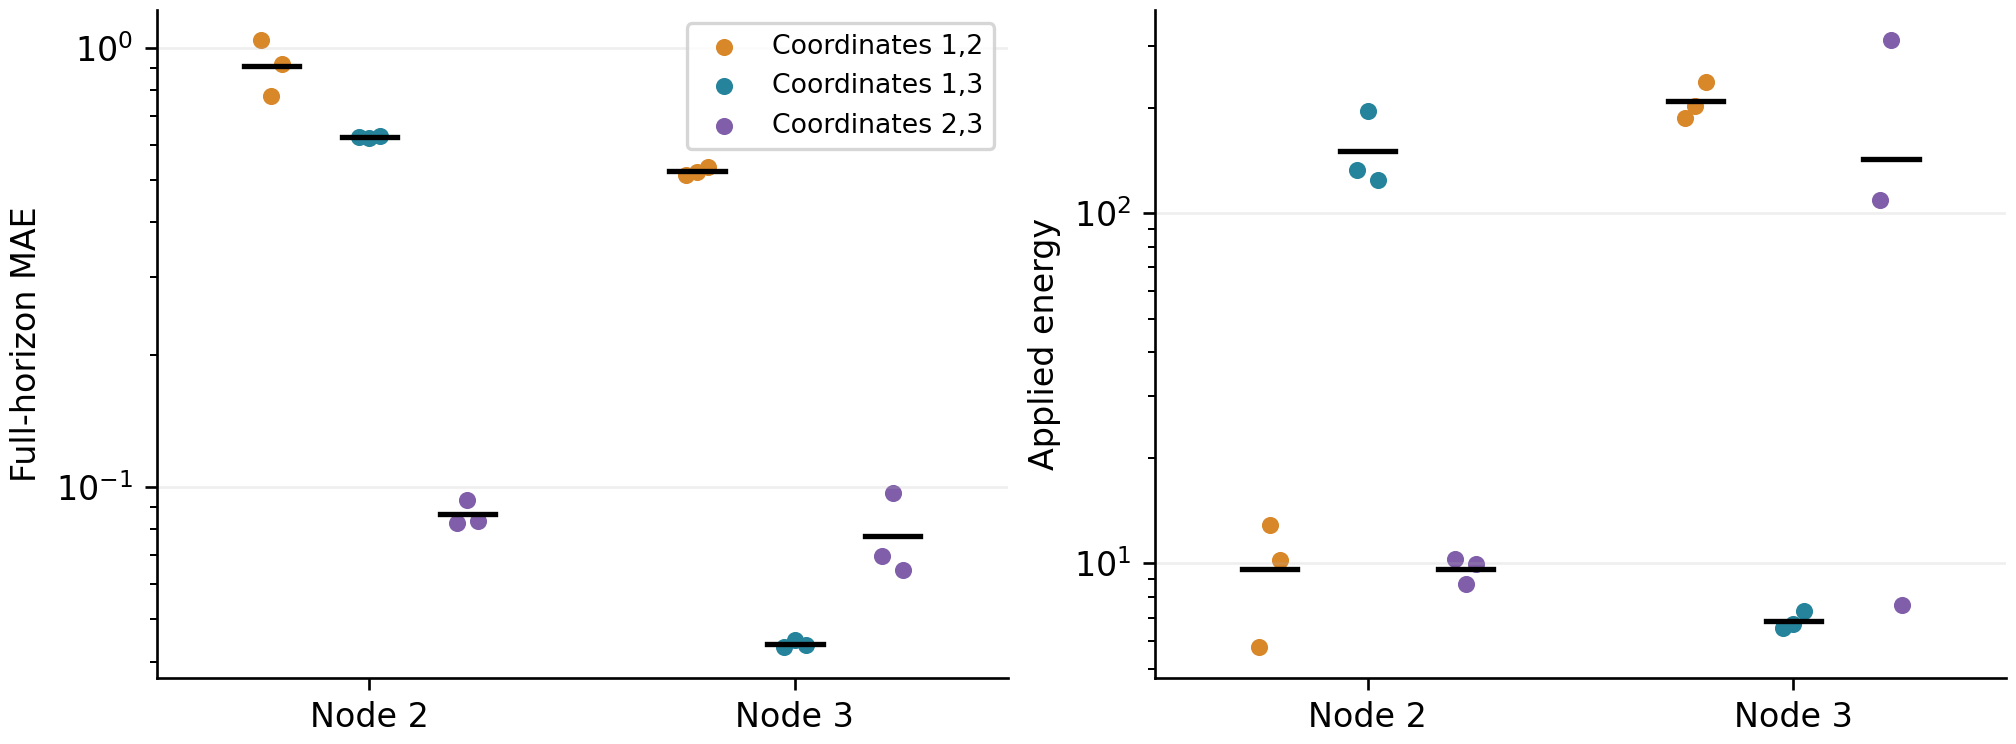
\includegraphics[width=0.92\textwidth]{figures/paired_observation_complete.png}
\caption{All paired four-dimensional subsets under single-node actuation. Each coordinate pair includes its drive states and error components. Points show individual training-run means; black marks indicate their average. Both error and energy are shown on logarithmic scales.}
\label{fig:observation_identity}
\end{figure*}

Table~\ref{tab:observation_identity} and Fig.~\ref{fig:observation_identity} confirm the actuator-dependent effect of coordinate composition. Node 2 performs best among these paired subsets with $\mathcal O_{23}$, whereas Node 3 favors $\mathcal O_{13}$ in both mean MAE and energy. The subsets omitting the actuated node's state--error pair, namely Node 2/$\mathcal O_{13}$ and Node 3/$\mathcal O_{12}$, give much larger residuals and energy than these favorable configurations. However, including that pair is not sufficient for low residuals: Node 2/$\mathcal O_{12}$ remains poor. Thus, the identity of the accompanying coordinate also matters. The results identify favorable observation combinations under the common finite-budget learning setup. At Node 3, $\mathcal O_{23}$ also exhibits substantial energy variability across training runs.

To check whether the direction of the observation-subset effect is specific to PPO, a targeted SAC comparison repeats the following pairs of four-dimensional observations: $\mathcal O_{12}$ versus $\mathcal O_{23}$ at Node 2, and $\mathcal O_{13}$ versus $\mathcal O_{23}$ at Node 3. Each configuration is trained independently in three runs at the same nominal budget of $4\times10^5$ transitions. The SAC settings used in the controller comparison below are unchanged apart from the observation input; no additional tuning or checkpoint selection is performed. All 12 final policies are evaluated deterministically on the same 20 initial conditions as the PPO paired-subset comparison. This check uses nominal dynamics only. The subsequent configuration-selection example uses PPO policies, so its candidate set is unchanged.

\begin{table}[pos=htbp,width=\linewidth]
\centering\small
\setlength{\tabcolsep}{3pt}
\caption{SAC four-dimensional observation cross-check. Values are mean $\pm$ sample SD across training-run means, using the same test initial conditions as the PPO comparison in Table~\ref{tab:observation_identity}.}
\label{tab:sac_observation_check}
\begin{tabular}{@{}clcc@{}}
\toprule
Node & Subset & MAE & $E_u$ \\
\midrule
2 & $\mathcal O_{12}$ & $0.4637\pm0.0659$ & $40.73\pm19.95$ \\
2 & $\mathcal O_{23}$ & $0.1350\pm0.0101$ & $7.17\pm0.69$ \\
3 & $\mathcal O_{13}$ & $0.0562\pm0.0067$ & $7.54\pm0.79$ \\
3 & $\mathcal O_{23}$ & $0.0840\pm0.0059$ & $10.57\pm0.54$ \\
\bottomrule
\end{tabular}
\end{table}

Table~\ref{tab:sac_observation_check} reproduces the direction of the PPO mean-error comparison. At Node 2, replacing $\mathcal O_{12}$ with $\mathcal O_{23}$ reduces SAC MAE from 0.4637 to 0.1350; at Node 3, replacing $\mathcal O_{13}$ with $\mathcal O_{23}$ increases it from 0.0562 to 0.0840. For each node, the same error ordering holds in all three SAC training runs. The agreement across PPO and SAC strengthens the evidence for placement-dependent observation preferences in the tested pairs. The SAC comparison focuses on these original and alternative subsets, complementing the complete paired-subset evaluation performed with PPO.

Control effort remains algorithm dependent. The Node 2 substitution reduces SAC energy from 40.73 to 7.17, whereas PPO energy changes little on average (9.60 to 9.64). At Node 3, energy increases for both algorithms, but the SAC increase (7.54 to 10.57) is much smaller than the PPO increase (6.85 to 142.70), which includes substantial training-run variability. Mean error ordering therefore transfers more consistently than the magnitude of the effort penalty. 

To illustrate how measured performance can inform a resource-constrained choice, an offline screening example uses a prespecified eight-candidate pool, fixed before the paired-subset completion. A candidate $c$ specifies the actuated node and its observation subset. The pool comprises Nodes 2 and 3, each with local two-dimensional observations, the original four-dimensional subset ($\mathcal O_{12}$ at Node 2 and $\mathcal O_{13}$ at Node 3), $\mathcal O_{23}$, and full six-dimensional observations. Each candidate retains all three training runs; configuration selection therefore accounts for variability across the retained runs. The allowed actuator set may be $\{2,3\}$, $\{2\}$, or $\{3\}$. The subsequently evaluated Node 2/$\mathcal O_{13}$ and Node 3/$\mathcal O_{12}$ configurations are not included among these eight candidates; the complete paired-subset comparison and this limited selection example answer different questions.

For a trajectory, let $z$ be the sample mean of $\|\mathbf e(t)\|_1$ over the final interval $16\leq t\leq20$. A trajectory passes when $z\leq\varepsilon$ and no state-protection boundary is reached. For training run $r$, its validation pass fraction is
\begin{equation}
 \widehat p_{c,r}(\varepsilon)
 =\frac{1}{n_v}\sum_{\ell=1}^{n_v}
 \mathbf 1\{z_{c,r,\ell}\leq\varepsilon,\ g_{c,r,\ell}=0\},
 \label{eq:configuration_pass}
\end{equation}
where $g$ counts state-protection boundary hits. A candidate is feasible only if $\min_r\widehat p_{c,r}\geq0.90$. Among feasible candidates with allowed actuation, the rule first minimizes observation dimension and then validation mean applied energy $E_u$. Remaining ties are resolved by a fixed candidate ordering. If none is feasible, no configuration is selected. Thus, fewer observed variables take priority over lower energy once the accuracy requirement is met.

Three error tolerances, $\varepsilon\in\{0.01,0.05,0.10\}$, are chosen with reference to the preceding experiments and fixed before configuration selection. Each tolerance specifies an acceptable mean synchronization error over the final four time units. For each tolerance, the rule uses 20 common validation initial conditions to identify configurations that meet the pass-rate requirement and select among them. The selected configurations are then evaluated on 40 separate test initial conditions drawn from the same initial-state distribution. Neither the tolerances nor the selections are adjusted using the test results. The system dynamics, nominal parameters, action bounds, and policy parameters remain unchanged throughout this procedure.

\begin{table*}[pos=!t,width=\textwidth]
\centering
\caption{Configurations selected using validation data and evaluated on separate test initial conditions. Test pass fractions are the minimum across three training runs, each evaluated on the same 40 test initial conditions. Error and energy average initial conditions and runs. A dash denotes no selection and hence no corresponding test; grouped tolerances have identical outcomes.}
\label{tab:configuration_selection}
\small
\begin{tabular}{cccccc}
\toprule
Allowed nodes & $\varepsilon$ & Selected node / observations & Test pass & Test $z$ & Test $E_u$\\
\midrule
$\{2,3\}$ & 0.01 & -- & -- & -- & --\\
$\{2,3\}$ & 0.05, 0.10 & $3\,/\,\mathcal O_{13}$ & 100\% & 0.0086 & 5.03\\
$\{2\}$ & 0.01, 0.05 & -- & -- & -- & --\\
$\{2\}$ & 0.10 & $2\,/\,\mathcal O_{23}$ & 100\% & 0.0282 & 8.11\\
$\{3\}$ & 0.01 & -- & -- & -- & --\\
$\{3\}$ & 0.05, 0.10 & $3\,/\,\mathcal O_{13}$ & 100\% & 0.0086 & 5.03\\
\bottomrule
\end{tabular}
\end{table*}

Table~\ref{tab:configuration_selection} shows which configurations are selected for each error tolerance. When either Node 2 or Node 3 can be controlled, the rule selects Node 3 with $\mathcal O_{13}$ at tolerances 0.05 and 0.10. When only Node 2 can be controlled, it selects $\mathcal O_{23}$ at 0.10. Every test trajectory of the selected configurations meets its corresponding error tolerance. At the stricter tolerance of 0.01, none of the eight candidates achieves the required validation pass rate.

Checking each training run separately avoids selecting a configuration whose average masks an unreliable run. For example, at tolerance 0.05, Node 2 with $\mathcal O_{23}$ has validation pass rates of 100\%, 75\%, and 100\%. Although their average exceeds 90\%, one run falls below the requirement, so this configuration is not selected at that tolerance. At tolerance 0.10, its selection over full observation reflects the priority given to fewer observed variables, rather than minimum energy: its validation mean energy is slightly higher than that of the six-dimensional configuration.

The procedure selects among the eight candidates according to nominal accuracy, observation dimension, and energy, then checks the choice on separate test initial conditions. Pass fractions describe the tested policies and sampled initial conditions; they do not establish the same pass rates for all possible initial conditions or newly trained policies. The tail-mean criterion measures average late-stage accuracy, whereas pointwise error limits and application-specific recovery requirements call for their own acceptance criteria. Shared initial conditions provide paired comparisons across policies.

Using the same validation data, changing the required per-run pass fraction from 90\% to 80\% or 100\% leaves the selections unchanged. Giving energy priority over observation dimension changes only the Node 2 choice at $\varepsilon=0.10$, from $\mathcal O_{23}$ to full observations. This illustrates why the resource priority must be stated explicitly; the candidate set and configurations chosen for independent testing remain unchanged.

We then examine whether the nominal choices retain their requested accuracy when response parameters change. The original selected Node 2/$\mathcal O_{23}$ and Node 3/$\mathcal O_{13}$ policies are evaluated without changing their parameters at their respective tolerances 0.10 and 0.05. For 40 new common initial conditions, response weights are set to $W_r=W\odot(1+\eta U)$, where each entry of $U$ is sampled uniformly from $[-1,1]$ and $\eta\in\{0,0.01,0.03,0.05\}$. The drive system is unchanged. Each initial condition uses the same mismatch direction across amplitudes and policies; an independent random stream preserves identical initial states. Zero weights remain zero. No retraining or configuration reselection is performed.

\begin{table*}[pos=!t,width=\textwidth]
\centering
\caption{Performance of the selected configurations under response-weight mismatch, without retraining or reselection. Pass fractions are the minimum across three training runs, each evaluated on the same 40 new initial conditions. Mean tail error $z$ and energy $E_u$ average runs and initial conditions. Pass fractions track each configuration against its own previously fixed tolerance.}
\label{tab:configuration_transfer}
\small
\begin{tabular}{cccccc}
\toprule
Configuration & $\varepsilon$ & $\eta$ & Minimum pass & Mean $z$ & Mean $E_u$\\
\midrule
$2/\mathcal O_{23}$ & 0.10 & 0\% & 100.0\% & 0.0266 & 10.08\\
$2/\mathcal O_{23}$ & 0.10 & 1\% & 97.5\% & 0.0402 & 10.11\\
$2/\mathcal O_{23}$ & 0.10 & 3\% & 57.5\% & 0.0942 & 10.20\\
$2/\mathcal O_{23}$ & 0.10 & 5\% & 35.0\% & 0.1571 & 10.39\\
$3/\mathcal O_{13}$ & 0.05 & 0\% & 100.0\% & 0.0084 & 5.84\\
$3/\mathcal O_{13}$ & 0.05 & 1\% & 97.5\% & 0.0181 & 5.85\\
$3/\mathcal O_{13}$ & 0.05 & 3\% & 75.0\% & 0.0455 & 5.91\\
$3/\mathcal O_{13}$ & 0.05 & 5\% & 42.5\% & 0.0743 & 6.01\\
\bottomrule
\end{tabular}
\end{table*}

Table~\ref{tab:configuration_transfer} shows that both configurations retain a minimum pass fraction of 97.5\% at 1\% relative mismatch, but fall below the original 90\% requirement at 3\% and 5\%. No state-protection boundary is reached in these 960 trajectories. The drop in pass fraction identifies the sensitivity of the selected configurations to larger response-weight deviations and motivates incorporating the intended parameter range into configuration validation.


Having examined which feedback variables to retain under single-node actuation, we next assess the complementary resource choice: the number of actuators. To quantify the performance cost of restricting actuation to one node, nominal PPO synchronization is evaluated for every nonempty subset of the three nodes: $\{1\}$, $\{2\}$, $\{3\}$, $\{1,2\}$, $\{1,3\}$, $\{2,3\}$, and $\{1,2,3\}$. For a subset $\mathcal S$, the input matrix contains the corresponding columns of $I_3$, and the policy produces $|\mathcal S|$ actions. The six-dimensional observation, error-only reward, initial-state distribution, RK4 integration, policy hidden layers, PPO hyperparameters, and nominal training budget of $4\times10^5$ transitions are unchanged. Each configuration includes three independent training runs and is evaluated on 20 common test initial conditions. All seven configurations and all three final checkpoints per configuration are reported, including configurations with poor synchronization.

The same per-actuator bound $|u_j|\leq4$ is imposed in every configuration, while $E_u$ sums energy across all active channels. Thus, additional actuators provide both additional control directions and a larger admissible total input magnitude ($\|\mathbf u\|_2\leq4\sqrt{|\mathcal S|}$). The comparison therefore measures the joint effect of additional control directions and increased aggregate control authority. Only nominal synchronization is tested in this ablation. Actuator count quantifies the structural actuation requirement.

\begin{table*}[pos=!t,width=\textwidth]
\centering\normalsize
\setlength{\tabcolsep}{6pt}
\renewcommand{\arraystretch}{1.15}
\caption{Nominal PPO ablation over all nonempty actuator subsets. Values are mean $\pm$ SD across training-run means; energy is summed over all active inputs.}
\label{tab:multi_input_comparison}
\begin{tabular}{@{}ccccc@{}}
\toprule
Controlled nodes & Inputs & MAE & Steady L1 error & $E_u$ \\
\midrule
$\{1\}$ & 1 & $1.3937 \pm 0.0029$ & $4.2825 \pm 0.1571$ & $266.49 \pm 13.41$ \\
$\{2\}$ & 1 & $0.0930 \pm 0.0022$ & $0.0426 \pm 0.0131$ & $9.09 \pm 1.53$ \\
$\{3\}$ & 1 & $0.0431 \pm 0.0012$ & $0.0091 \pm 0.0033$ & $6.54 \pm 0.34$ \\
$\{1,2\}$ & 2 & $0.1145 \pm 0.0110$ & $0.0679 \pm 0.0212$ & $20.61 \pm 1.28$ \\
$\{1,3\}$ & 2 & $0.0232 \pm 0.0007$ & $0.0119 \pm 0.0019$ & $10.93 \pm 0.12$ \\
$\{2,3\}$ & 2 & $0.0205 \pm 0.0011$ & $0.0141 \pm 0.0040$ & $8.15 \pm 0.27$ \\
$\{1,2,3\}$ & 3 & $0.0118 \pm 0.0007$ & $0.0105 \pm 0.0026$ & $10.91 \pm 0.17$ \\
\bottomrule
\end{tabular}
\end{table*}

\begin{figure*}[pos=!t,width=\textwidth]
  \centering
  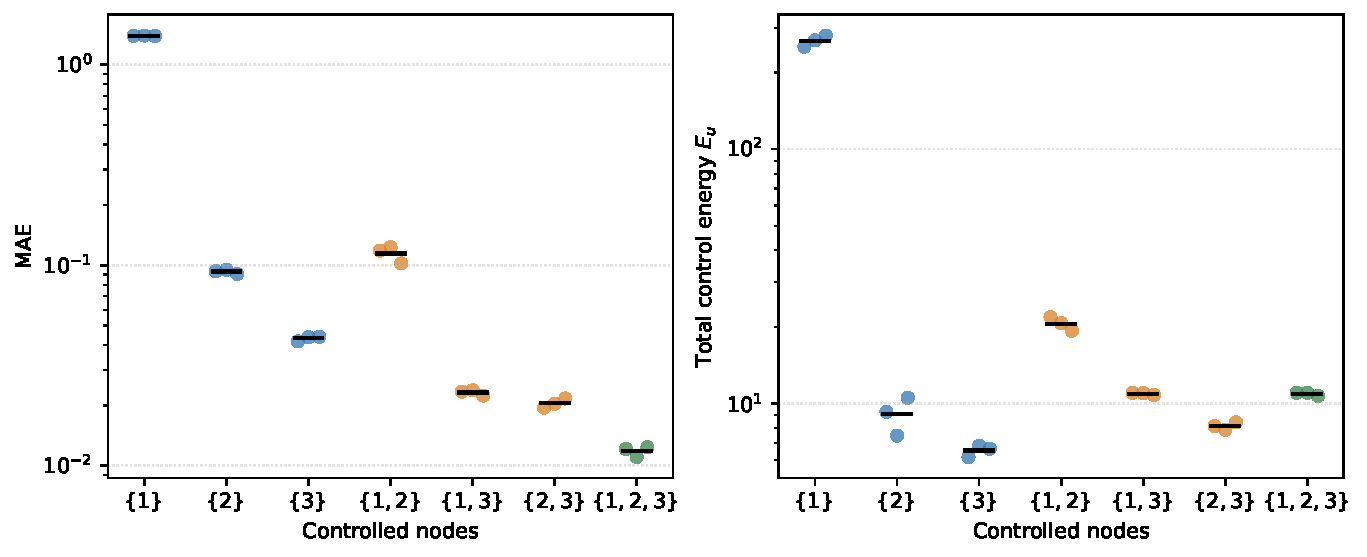
\includegraphics[width=\textwidth]{figures/multi_input_matched_budget.pdf}
  \caption{Nominal synchronization error and total control energy for all actuator subsets. Colored points show individual training-run means; black horizontal marks indicate their average. Blue, orange, and green indicate one, two, and three actuators, respectively.}
  \label{fig:multi_input_comparison}
\end{figure*}

Table~\ref{tab:multi_input_comparison} and Fig.~\ref{fig:multi_input_comparison} quantify the tradeoff. Single-node control at Node 3 gives MAE 0.0431 and energy 6.54, whereas $\{2,3\}$ gives 0.0205 and 8.15 and $\{1,2,3\}$ gives 0.0118 and 10.91. Thus, one actuator retains low-residual synchronization with lower measured energy, but incurs a higher full-horizon error than these multi-input configurations. The steady L1 error does not decrease monotonically with actuator count: it is 0.0091 for $\{3\}$, compared with 0.0141 for $\{2,3\}$ and 0.0105 for $\{1,2,3\}$. Full-horizon accuracy and steady-state precision thus capture different consequences of increasing actuator availability.

The $\{1,2\}$ configuration has higher MAE and energy than $\{2\}$ under the fixed training budget, while configurations containing Node 3 perform better in full-horizon MAE. This emphasizes the effect of actuator placement and finite-budget policy optimization. Although adding an actuator enlarges the admissible control set, exploiting that flexibility also depends on policy optimization within the available training budget. These results quantify the accuracy--effort tradeoff of single-input control as a resource-constrained design choice.

\subsection{Controller Comparison and Robustness Assessment}
\label{subsec:robustness_tests}

The preceding experiments examine where to apply control and which variables to observe. We now assess how the resulting single-input PPO controllers compare with traditional feedback and SAC under nominal dynamics, parameter mismatch, impulses, and process noise. These comparisons test the performance and limitations of the learned feedback rather than seek a controller that is best in every setting. The scenario curves use the reference LQR weight $R=1$; Table~\ref{tab:lqr_weight_sensitivity} additionally reports LQR with a weight selected using validation data.


For the LQR baseline, $Q=I_3$ is fixed and $R$ is selected from $\{0.01,0.1,1,10,100\}$ using ten validation initial conditions and the normalized-MAE score specified for SMC. Both nodes select $R=0.01$, which is kept fixed for the 20 separate test initial conditions. This selection includes nominal, mismatch, and impulse scenarios and does not penalize energy, whereas PPO training uses nominal dynamics only.

\begin{table*}[pos=!t,width=\textwidth]
\centering
\normalsize
\setlength{\tabcolsep}{6pt}
\renewcommand{\arraystretch}{1.15}
\caption{Synchronization error and control energy of PPO and LQR. Both the reference weight $R=1$ and the validation-selected weight $R=0.01$ are reported. MAE covers the full simulation interval, including the impulse scenario.}
\label{tab:lqr_weight_sensitivity}
\begin{tabular}{@{}clrrrrrr@{}}
\toprule
 & & \multicolumn{2}{c}{PPO} & \multicolumn{2}{c}{LQR, $R=1$} & \multicolumn{2}{c}{LQR, $R=0.01$} \\
Node & Scenario & MAE & $E_u$ & MAE & $E_u$ & MAE & $E_u$ \\
\midrule
2 & Nominal & 0.0930 & 9.09 & 0.0907 & 3.78 & 0.0772 & 10.58 \\
2 & $\eta=2$ & 0.1703 & 11.85 & 0.2330 & 5.58 & 0.1486 & 14.60 \\
2 & Impulse & 0.4339 & 17.51 & 0.5128 & 9.95 & 0.3368 & 31.23 \\
2 & $\sigma=0.05$ & 0.2669 & 135.57 & 0.3742 & 11.67 & 0.2427 & 90.27 \\
\midrule
3 & Nominal & 0.0431 & 6.54 & 0.0510 & 2.65 & 0.0392 & 4.99 \\
3 & $\eta=2$ & 0.0656 & 6.44 & 0.0989 & 3.56 & 0.0647 & 5.29 \\
3 & Impulse & 0.2581 & 18.09 & 0.3330 & 7.49 & 0.2592 & 13.71 \\
3 & $\sigma=0.05$ & 0.1312 & 69.96 & 0.1826 & 7.11 & 0.1264 & 23.27 \\
\bottomrule
\end{tabular}
\end{table*}

Table~\ref{tab:lqr_weight_sensitivity} compares PPO with the reference and selected LQR settings. At Node 2, LQR with $R=0.01$ achieves lower full-horizon MAE in all four settings, but uses more energy under mismatch and impulse disturbance. Under nominal dynamics and noise, it has both lower MAE and lower energy than PPO.

At Node 3, the selected LQR has lower mean error and energy under nominal dynamics, mismatch, and noise. PPO has slightly lower post-impulse error but uses more energy. Thus, the learned controller does not uniformly outperform model-based feedback; its performance must be considered alongside the actuator and observation choices studied above.


We next examine how the controllers with unchanged parameters respond as model uncertainty increases~\cite{zhang2011weak}. The drive dynamics remain unchanged, while uncertainty in the response system is introduced through its weight matrix:
\begin{equation}
	W_r = W + \eta (W\odot \Delta),
	\label{eq:mismatch_matrix}
\end{equation}
where $\eta$ denotes the mismatch intensity coefficient, $\odot$ denotes the Hadamard product, and $\Delta=[\delta_{ij}]$ is a random perturbation matrix with
\begin{equation}
	\delta_{ij}\sim U(-0.03,0.03).
	\label{eq:mismatch_delta}
\end{equation}
This formulation corresponds to a relative multiplicative mismatch. That is, each nonzero connection weight in the response system is perturbed around its nominal value, while zero entries remain unchanged. This modeling approach preserves the original network topology and is also consistent with practical parameter deviations caused by manufacturing errors, calibration bias, and component tolerances.

It should be noted that $\eta$ is a normalized scaling coefficient rather than the direct percentage of mismatch. When $\eta=1.0$, the relative perturbation range is approximately $\pm 3\%$ of the original weight; when $\eta=2.0$, the range is approximately $\pm 6\%$. In this work, the following mismatch levels are considered:
\begin{equation}
	\eta\in\{0.0,0.5,1.0,1.5,2.0\}.
	\label{eq:mismatch_levels}
\end{equation}
Here, $\eta=0.0$ corresponds to the nominal case without mismatch, while larger values represent stronger parameter uncertainty.

All controllers are evaluated without adaptation under the perturbed response matrices. PPO is trained without domain randomization; LQR is designed from the nominal linearization, and SMC uses nominal compensation with parameters selected on separate validation scenarios as described above.

At $\eta=2$, PPO has lower Node 2 MAE than fixed-gain feedback, SMC, and the reference LQR, but not the validation-selected LQR or SAC. The selected LQR achieves its lower error with more energy than PPO, whereas SAC uses less energy. Node 3 generally shows smaller absolute error differences. Figure~\ref{fig:mismatch_methods} and Table~\ref{tab:traditional_summary} report the reference-controller results; Tables~\ref{tab:lqr_weight_sensitivity} and~\ref{tab:sac_comparison} provide the selected LQR and SAC comparisons.

\begin{figure*}[pos=!t,width=\textwidth]
	\centering
	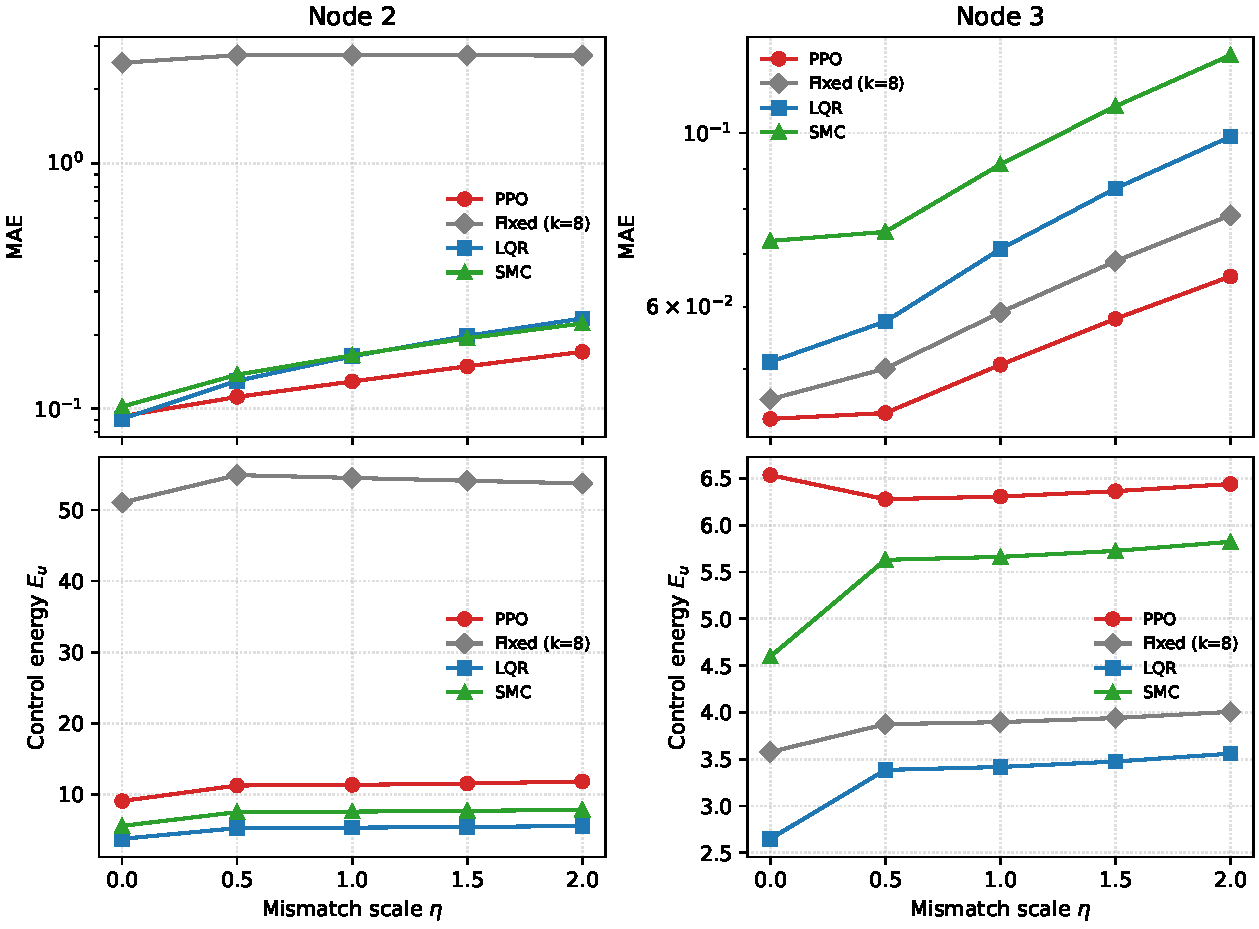
\includegraphics[width=\textwidth]{figures/mismatch_methods.pdf}
	\caption{MAE and control energy of PPO, fixed-gain feedback ($k=8$), LQR, and SMC under parameter mismatch. Curves show mean synchronization error and control energy.}
	\label{fig:mismatch_methods}
\end{figure*}

\begin{table*}[pos=!t,width=\textwidth]
	\centering
	\normalsize
	\setlength{\tabcolsep}{6pt}
	\renewcommand{\arraystretch}{1.10}
	\caption{Representative mismatch and impulse-disturbance results.}
	\label{tab:traditional_summary}
	\begin{tabular}{@{}clccccc@{}}
		\toprule
		\multirow{2}{*}{Node} & \multirow{2}{*}{Method} & \multicolumn{2}{c}{Nominal} & \multicolumn{1}{c}{$\eta=2$} & \multicolumn{2}{c}{Impulse} \\
		\cmidrule(lr){3-4}\cmidrule(lr){5-5}\cmidrule(lr){6-7}
		& & MAE & $E_u$ & MAE & $E_{\mathrm{post}}$ & $E_u$ \\
		\midrule
		\multirow{4}{*}{2}
		& PPO & 0.0930 & 9.09 & 0.1703 & 2.0800 & 17.51 \\
		& Fixed ($k=8$) & 2.5673 & 51.03 & 2.7481 & 8.6188 & 74.02 \\
		& LQR & 0.0907 & 3.78 & 0.2330 & 2.5264 & 9.95 \\
		& SMC & 0.1018 & 5.59 & 0.2223 & 2.7691 & 14.13 \\
		\midrule
		\multirow{4}{*}{3}
		& PPO & 0.0431 & 6.54 & 0.0656 & 1.2969 & 18.09 \\
		& Fixed ($k=8$) & 0.0457 & 3.58 & 0.0785 & 1.2518 & 16.21 \\
		& LQR & 0.0510 & 2.65 & 0.0989 & 1.6883 & 7.49 \\
		& SMC & 0.0728 & 4.60 & 0.1257 & 1.7352 & 11.37 \\
		\bottomrule
	\end{tabular}
\end{table*}


In addition to parameter uncertainty, sudden impulse disturbance is also considered to evaluate the transient recovery capability of the controllers~\cite{cao2024synchronisation}. In the testing implementation, an impulse is added to all three drive-state components immediately after integration at step 200 ($t=10$); the response state is not directly shifted. This tests recovery following an abrupt change of the synchronization reference. The impulse vector is set as
\begin{equation}
	\mathbf{p}=[5,5,5]^{\mathrm T}.
	\label{eq:pulse_vector}
\end{equation}
The same drive-state jump is applied for both actuator locations and all controllers. It tests recovery after a shared reference change; the resulting response can still depend on the chosen jump direction.

Because the imposed jump largely determines the immediate peak $M_p$, recovery is assessed using $E_{\mathrm{post}}$ together with energy. At Node 2, PPO recovers with lower mean error than fixed-gain feedback and SMC. The selected LQR and SAC achieve lower recovery error than PPO but use more energy; SAC also shows greater variation across training runs. At Node 3, the mean recovery errors of fixed-gain feedback, PPO, and the selected LQR are close, with lower energy for LQR. Figure~\ref{fig:pulse_methods} and Table~\ref{tab:traditional_summary} show the reference settings, including LQR with $R=1$.

\begin{figure*}[pos=!t,width=\textwidth]
	\centering
	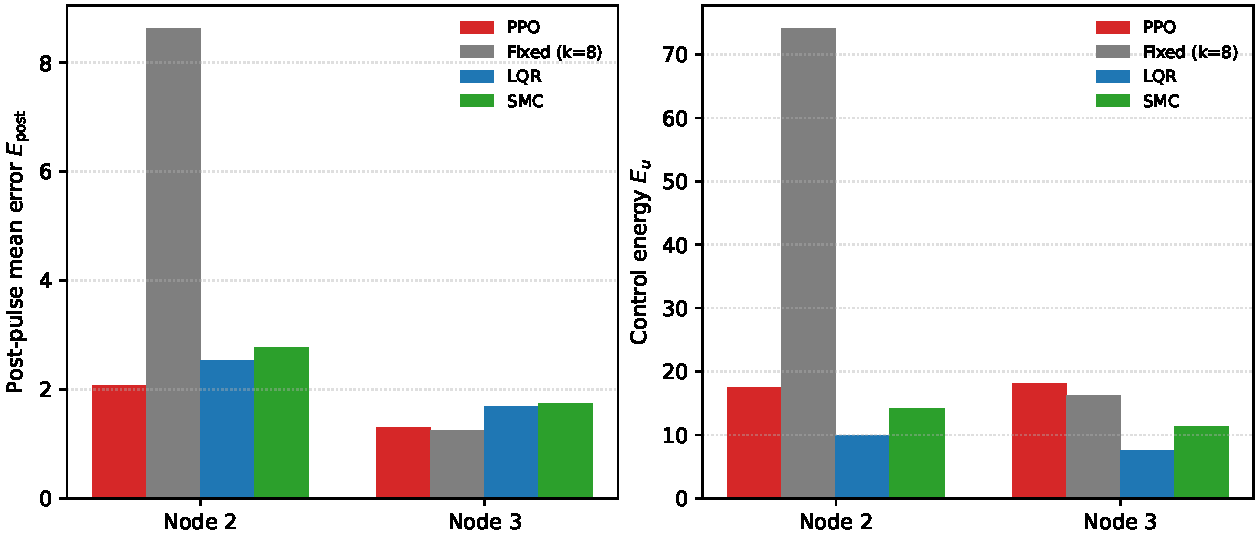
\includegraphics[width=\textwidth]{figures/pulse_methods.pdf}
	\caption{Post-pulse mean error and control energy for the reference settings under the same global impulse. LQR uses $R=1$.}
	\label{fig:pulse_methods}
\end{figure*}


To further evaluate the robustness of the learned controller under persistent random perturbations, zero-mean Gaussian noise is added to the response system during testing, while the training stage remains noise-free. This setting tests the trained policy with its parameters held fixed under stochastic state perturbations absent from training. Specifically, after each control step and numerical integration, additive Gaussian noise is imposed on the response state:
\begin{equation}
	\mathbf{y}_{k+1}^{\mathrm{noisy}}
	=
	\mathbf{y}_{k+1}
	+
	\boldsymbol{\xi}_k,
	\label{eq:gaussian_noise_state}
\end{equation}
where
\begin{equation}
	\boldsymbol{\xi}_k\sim \mathcal{N}(\mathbf{0},\sigma^2 I_3).
	\label{eq:gaussian_noise_distribution}
\end{equation}
Here, $\sigma$ denotes the noise intensity and $I_3$ is the $3\times 3$ identity matrix. The tested noise levels are
\begin{equation}
	\sigma\in\{0,0.01,0.02,0.05\}.
	\label{eq:noise_levels}
\end{equation}

At $\sigma=0.05$, the selected LQR has lower Node 2 mean MAE and energy than PPO, while SAC has similar MAE and lower energy. PPO has lower MAE than SMC and the reference LQR. Figure~\ref{fig:noise_methods} and Table~\ref{tab:noise_summary} show how the reference controllers respond to increasing noise. Since noise is added to the evolving response state rather than only to its measurements, these results describe sensitivity to process noise.

\begin{figure*}[pos=!t,width=\textwidth]
	\centering
	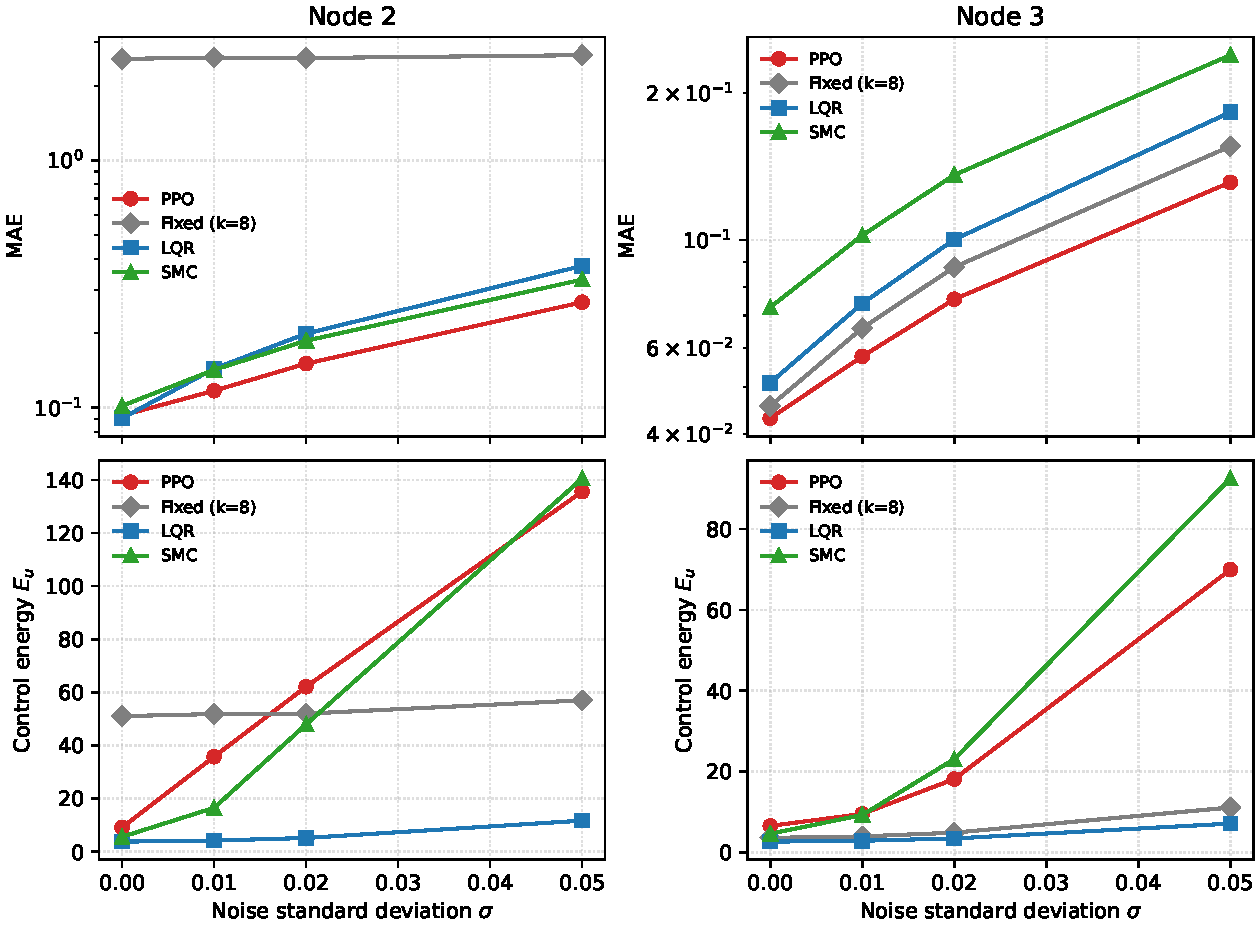
\includegraphics[width=\textwidth]{figures/noise_methods.pdf}
	\caption{MAE and control energy of the four reference controllers under Gaussian-noise perturbation. LQR uses $R=1$.}
	\label{fig:noise_methods}
\end{figure*}

\begin{table}[pos=h,width=\linewidth]
	\centering
	\setlength{\tabcolsep}{3pt}
	\renewcommand{\arraystretch}{1.10}
	\caption{Performance at the highest tested noise intensity, $\sigma=0.05$.}
	\label{tab:noise_summary}
	\begin{tabular}{@{}clccc@{}}
		\toprule
		Node & Method & MAE & Steady L1 error & $E_u$ \\
		\midrule
		\multirow{4}{*}{2}
		& PPO & 0.2669 & 0.5383 & 135.57 \\
		& Fixed ($k=8$) & 2.6584 & 8.7280 & 56.99 \\
		& LQR & 0.3742 & 0.8979 & 11.67 \\
		& SMC & 0.3295 & 0.7298 & 140.49 \\
		\midrule
		\multirow{4}{*}{3}
		& PPO & 0.1312 & 0.3183 & 69.96 \\
		& Fixed ($k=8$) & 0.1555 & 0.4000 & 11.09 \\
		& LQR & 0.1826 & 0.4419 & 7.11 \\
		& SMC & 0.2389 & 0.6029 & 92.51 \\
		\bottomrule
	\end{tabular}
\end{table}


To assess the dependence of the results on the learning algorithm, SAC~\cite{haarnoja2018soft} is evaluated on the same single-input Node 2 and Node 3 tasks. Both algorithms use the six-dimensional observation $(\mathbf x,\mathbf e)/5$, reward $-0.1\|\mathbf e\|_1$, actuator bound $|u|\leq4$, nominal training dynamics, and final checkpoints at a nominal budget of $4\times10^5$ environment transitions. Three independent training runs and 20 common test initial conditions per seed are used. All checkpoints are retained, and evaluation uses deterministic actions without online learning. The compared test settings are nominal dynamics, mismatch $\eta=2$, the drive-state impulse at $t=10$, and response process noise with $\sigma=0.05$.

Both implementations use two hidden layers of width 64, a learning rate of $3\times10^{-4}$, batch size 128, and discount factor 0.99. PPO uses hyperbolic tangent hidden activations, four environments with 512 steps per rollout, ten optimization epochs, clip range 0.2, GAE parameter 0.95, and entropy coefficient 0.001. SAC uses rectified linear unit (ReLU) hidden activations, one environment, a replay buffer of $10^5$ transitions, 5,000 initial exploration steps, one gradient update per subsequent transition, target-update coefficient $\tau=0.005$, and automatic entropy adjustment with target entropy $-1$. These settings are fixed across nodes and seeds. The budget matches environment interactions; gradient-update counts and training times follow each algorithm\'s update schedule. The comparison uses these fixed hyperparameter settings.

\begin{table*}[pos=!t,width=\textwidth]
\centering\normalsize
\setlength{\tabcolsep}{5pt}
\renewcommand{\arraystretch}{1.15}
\caption{PPO and SAC at the same nominal budget of $4\times10^5$ environment transitions. Values are mean $\pm$ sample SD across training-run means. $E_{\mathrm{post}}$ is reported only for the impulse scenario.}
\label{tab:sac_comparison}
\begin{tabular}{@{}cllccc@{}}
\toprule
Node & Scenario & Method & MAE & $E_u$ & $E_{\mathrm{post}}$ \\
\midrule
2 & Nominal & PPO & $0.0930 \pm 0.0022$ & $9.09 \pm 1.53$ & -- \\
2 & Nominal & SAC & $0.1173 \pm 0.0046$ & $6.27 \pm 0.45$ & -- \\
2 & $\eta=2$ & PPO & $0.1703 \pm 0.0085$ & $11.85 \pm 1.60$ & -- \\
2 & $\eta=2$ & SAC & $0.1513 \pm 0.0037$ & $9.31 \pm 0.43$ & -- \\
2 & Impulse & PPO & $0.4339 \pm 0.0246$ & $17.51 \pm 1.19$ & $2.0800 \pm 0.1451$ \\
2 & Impulse & SAC & $0.4206 \pm 0.0979$ & $25.20 \pm 9.79$ & $1.9226 \pm 0.5913$ \\
2 & $\sigma=0.05$ & PPO & $0.2669 \pm 0.0049$ & $135.57 \pm 48.71$ & -- \\
2 & $\sigma=0.05$ & SAC & $0.2632 \pm 0.0052$ & $86.13 \pm 8.86$ & -- \\
\midrule
3 & Nominal & PPO & $0.0431 \pm 0.0012$ & $6.54 \pm 0.34$ & -- \\
3 & Nominal & SAC & $0.0416 \pm 0.0010$ & $4.60 \pm 0.11$ & -- \\
3 & $\eta=2$ & PPO & $0.0656 \pm 0.0025$ & $6.44 \pm 0.30$ & -- \\
3 & $\eta=2$ & SAC & $0.0644 \pm 0.0009$ & $5.07 \pm 0.16$ & -- \\
3 & Impulse & PPO & $0.2581 \pm 0.0003$ & $18.09 \pm 3.50$ & $1.2969 \pm 0.0070$ \\
3 & Impulse & SAC & $0.2735 \pm 0.0106$ & $12.62 \pm 0.53$ & $1.3987 \pm 0.0664$ \\
3 & $\sigma=0.05$ & PPO & $0.1312 \pm 0.0066$ & $69.96 \pm 17.55$ & -- \\
3 & $\sigma=0.05$ & SAC & $0.1273 \pm 0.0013$ & $50.40 \pm 14.21$ & -- \\
\bottomrule
\end{tabular}
\end{table*}

\begin{figure*}[pos=!t,width=\textwidth]
  \centering
  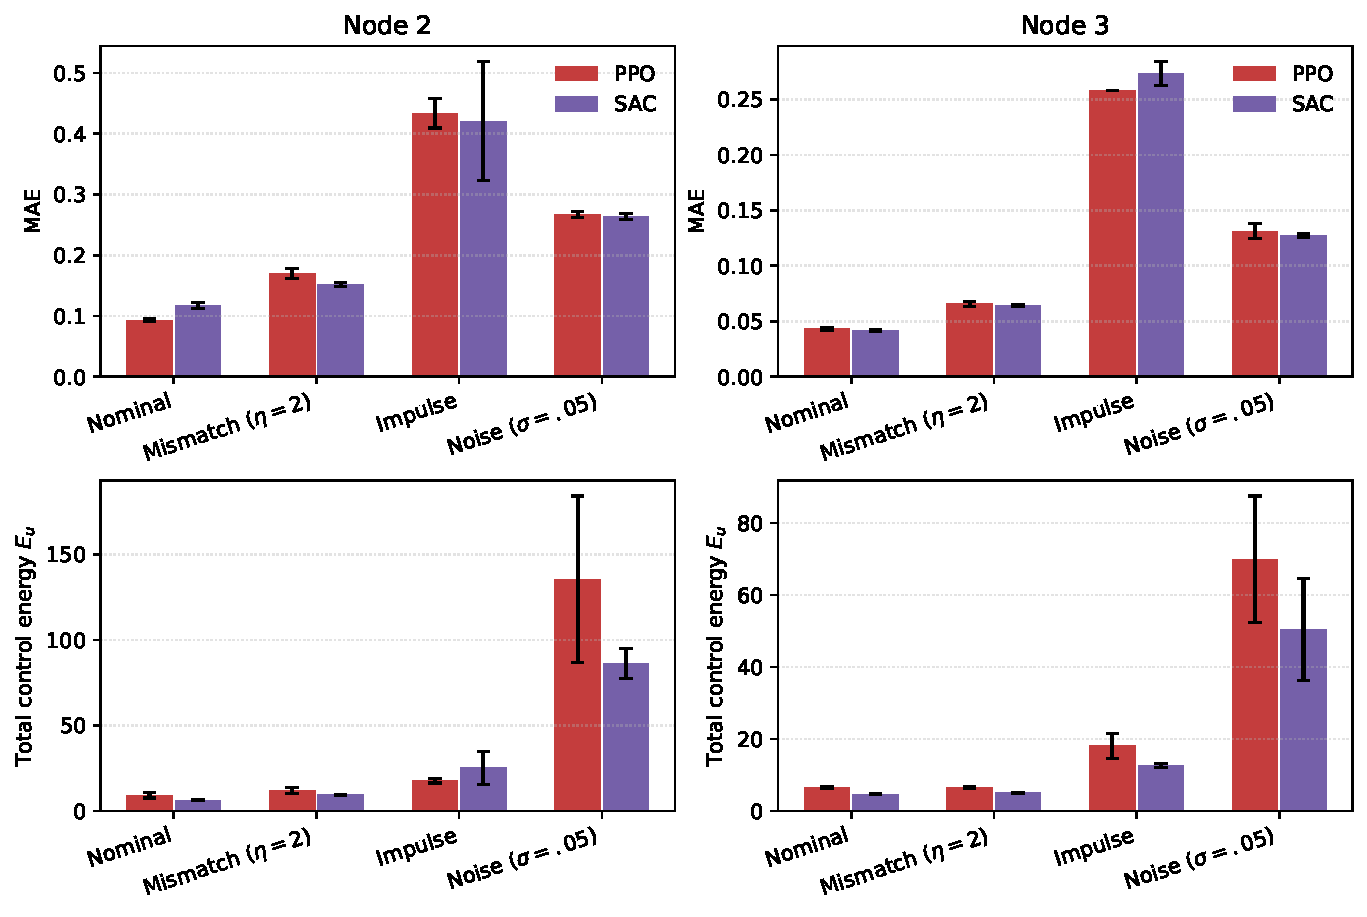
\includegraphics[width=\textwidth]{figures/ppo_sac_matched_budget.pdf}
  \caption{PPO--SAC comparison at matched environment-transition budgets. Bars show averages across training-run means; error bars indicate their sample standard deviation. The upper panels use full-horizon MAE for every scenario; the separate post-impulse metric is given in Table~\ref{tab:sac_comparison}.}
  \label{fig:sac_comparison}
\end{figure*}

Table~\ref{tab:sac_comparison} and Fig.~\ref{fig:sac_comparison} show that neither learning algorithm gives the best result in every setting. At Node 2, PPO has lower nominal MAE, whereas SAC has lower MAE and energy under mismatch. After the impulse, SAC achieves lower mean recovery error but uses more energy and varies more across training runs. Under noise, their mean MAEs are close, with lower energy for SAC.

At Node 3, SAC has slightly lower mean MAE under nominal dynamics, mismatch, and noise, and lower energy in all four settings. PPO has lower post-impulse error. These differences qualify the performance of the chosen PPO implementation. More importantly for the observation-design question, the separate matched-subset SAC experiment reproduces the direction of the observation effects at both nodes.

The comparisons point to a practical distinction between actuator location and observation content. Node 2 benefits substantially from changing the four-dimensional subset, while Node 3 favors a different pair. The SAC check reproduces the direction of these error changes, strengthening the case for selecting feedback variables in relation to the actuated coordinate. The useful question is therefore not simply how many variables to retain, but which variables support the desired accuracy at the available actuator.

The configuration-selection example shows how to use this finding in controller design. The rule first excludes configurations that fail the accuracy requirement, then selects the smallest observation dimension and uses energy to distinguish equally sized configurations. Its mismatch tests show why a choice made under nominal conditions should be checked over the intended operating range. Adding actuators offers a different route to improved full-horizon accuracy, but also increases available control authority and measured total effort. Accuracy and applied effort can therefore be competing design requirements~\cite{rodriguez2020multiobjective}, even though the PPO reward used here optimizes error alone.

The controller comparisons establish the context for these design findings: PPO provides one learned implementation of bounded single-input feedback, not a uniformly superior alternative to LQR, SMC, or SAC. The main result concerns how actuator location and observation content interact, together with the accuracy and energy changes caused by adding control channels. Its scope is the stated three-state network, available measurements, and separately tested perturbations; other networks and combined disturbances require further evaluation.

% Allow the next section to fill available space while pending floats are placed.
\begingroup
\let\FloatBarrier\relax
\section{Image Encryption Scheme and Statistical Security Analysis}
\label{sec:image_encry}
\endgroup

\subsection{Encryption Scheme}

Astronomical observation systems generate large amounts of high-value image data, including celestial structures, planetary surfaces, and remote-sensing information. In distributed observation scenarios such as Very Long Baseline Interferometry~\cite{thompson2017interferometry}, these images may need to be transmitted and shared across different observation sites, making them vulnerable to eavesdropping, tampering, and unauthorized access. Therefore, secure image protection is important for astronomical and space-related data applications.

\begin{figure*}[pos=!t,width=\textwidth]
\centering
	\setlength{\tabcolsep}{6pt}
	\begin{tabular}{ccc}
		
\includegraphics[width=0.28\textwidth]{figures/manuscript_a/original_image.jpg} &
		
\includegraphics[width=0.28\textwidth]{figures/manuscript_a/cipher_image.png} &
		
\includegraphics[width=0.28\textwidth]{figures/manuscript_a/decrypted_image.png} \\[-1mm]
		(a) Original & (b) Encrypted & (c) Decrypted
	\end{tabular}
	
	\caption{The original, encrypted, and decrypted images.}
	\label{fig:full_fig}
\end{figure*}

Astronomical images usually contain rich textures, complex intensity distributions, and strong spatial correlations among adjacent pixels, making them suitable test objects for image encryption algorithms. An effective encryption scheme should conceal the visual content of the original image and reduce its statistical redundancy. Since chaotic systems are sensitive to initial conditions and can generate pseudo-random trajectories, they have been widely used for image encryption. In a drive--response synchronization framework, synchronized chaotic trajectories can provide consistent key streams for encryption and decryption.

Motivated by this idea, this chapter applies the synchronized trajectories generated by the PPO-controlled continuous-time Hopfield chaotic neural network to image encryption. The flow chart of our method in image encryption is shown in Fig.~\ref{fig:encrypt_process}. The proposed scheme combines synchronized Hopfield chaotic sequences, Logistic-map-based diffusion, and dynamic DNA coding. The plain image is first encrypted and then decrypted to verify reversibility. The RGB histogram and adjacent-pixel correlation are further analyzed to evaluate the statistical security of the encrypted image. The specific steps of encryption are as follows:
%\begin{figure}[!htbp]
%	\centering
%	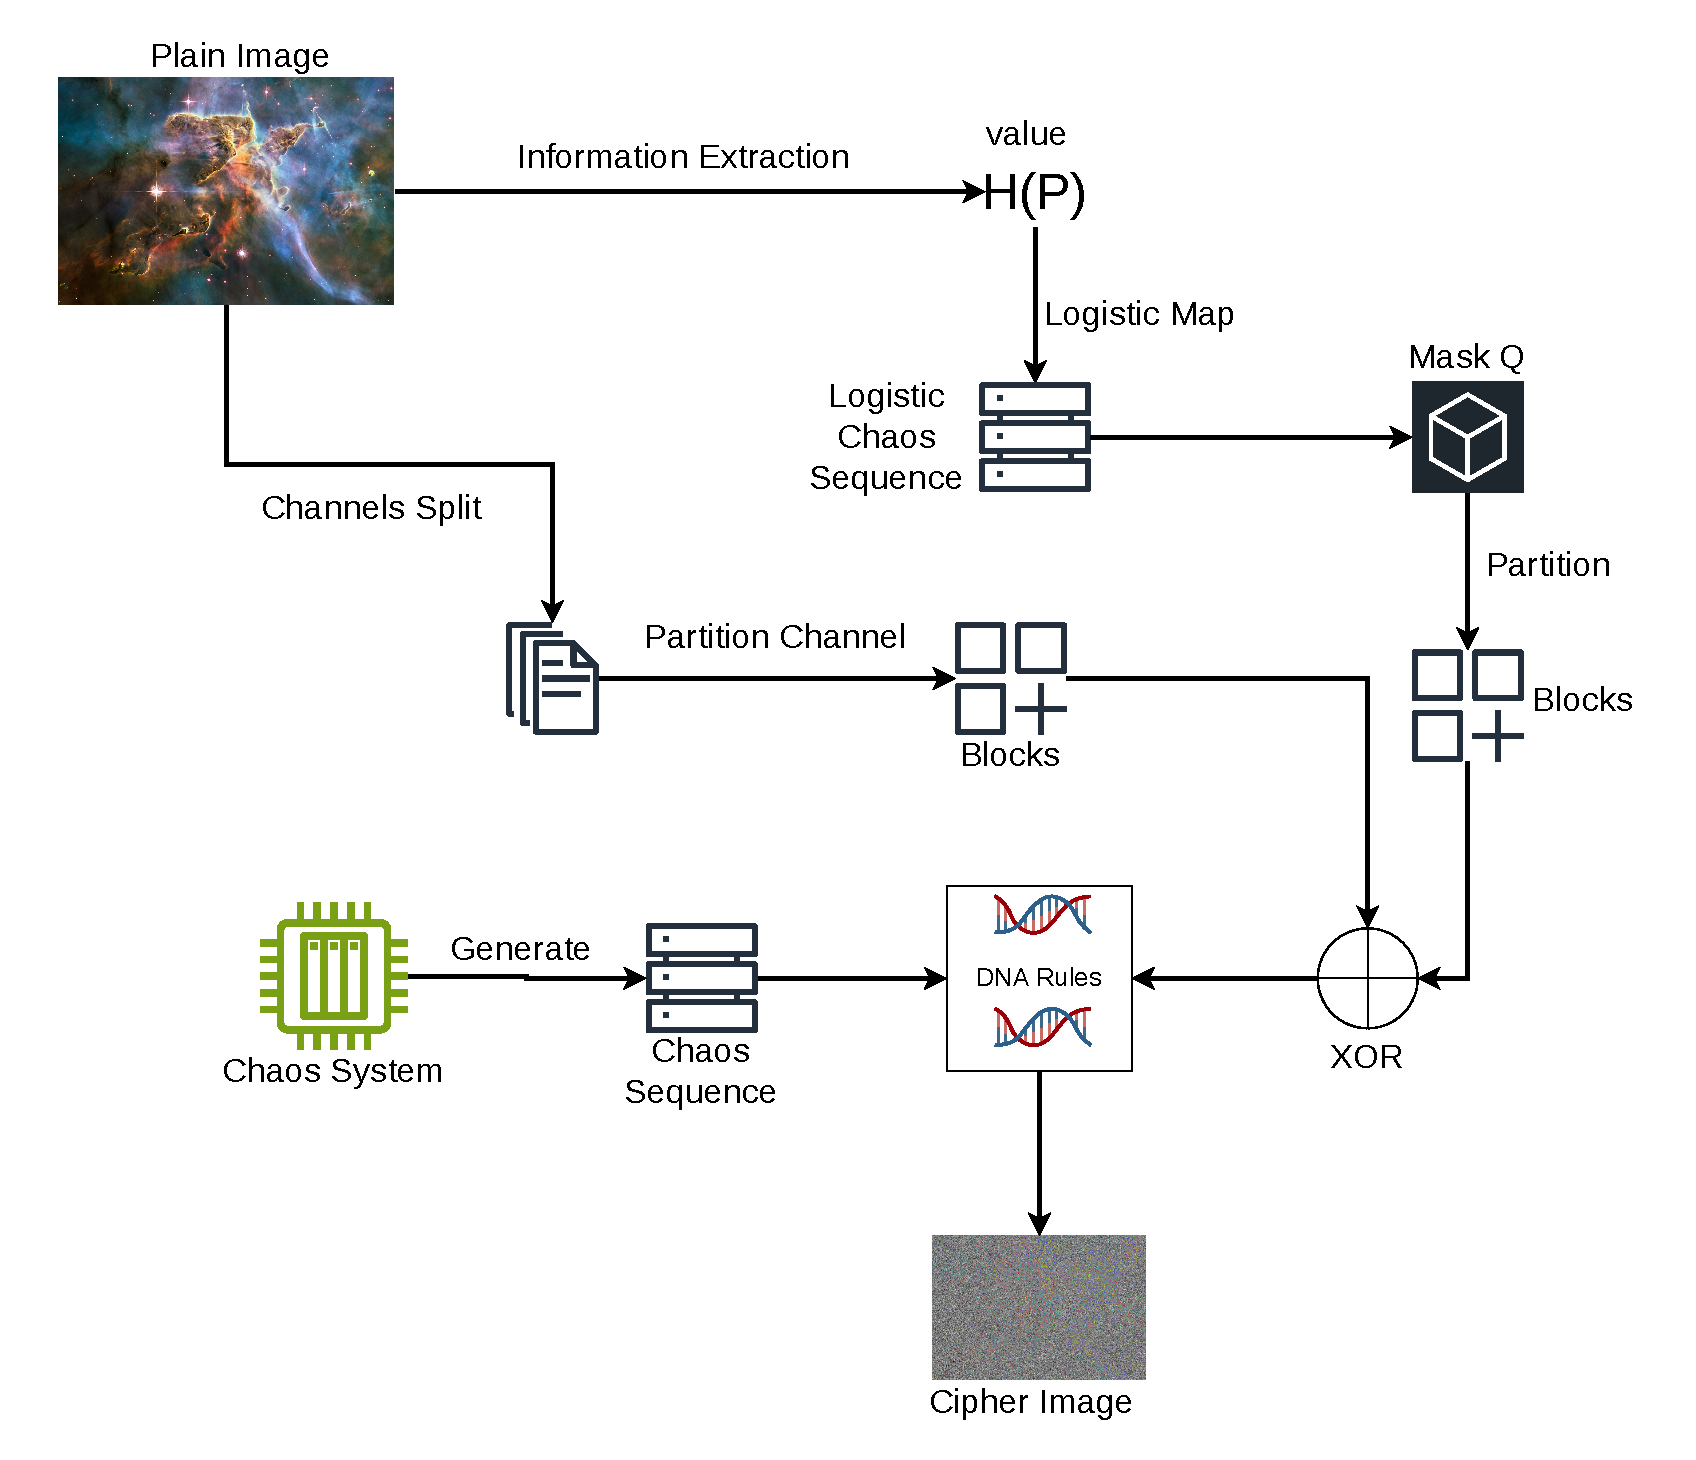
\includegraphics[width=\linewidth,keepaspectratio]{figures/manuscript_a/encrypt_process.pdf}
%	\caption{Flowchart of the image encryption process.}
%	\label{fig:encrypt_process}
%\end{figure}

\begin{figure*}[pos=!t,width=\textwidth]
\centering
	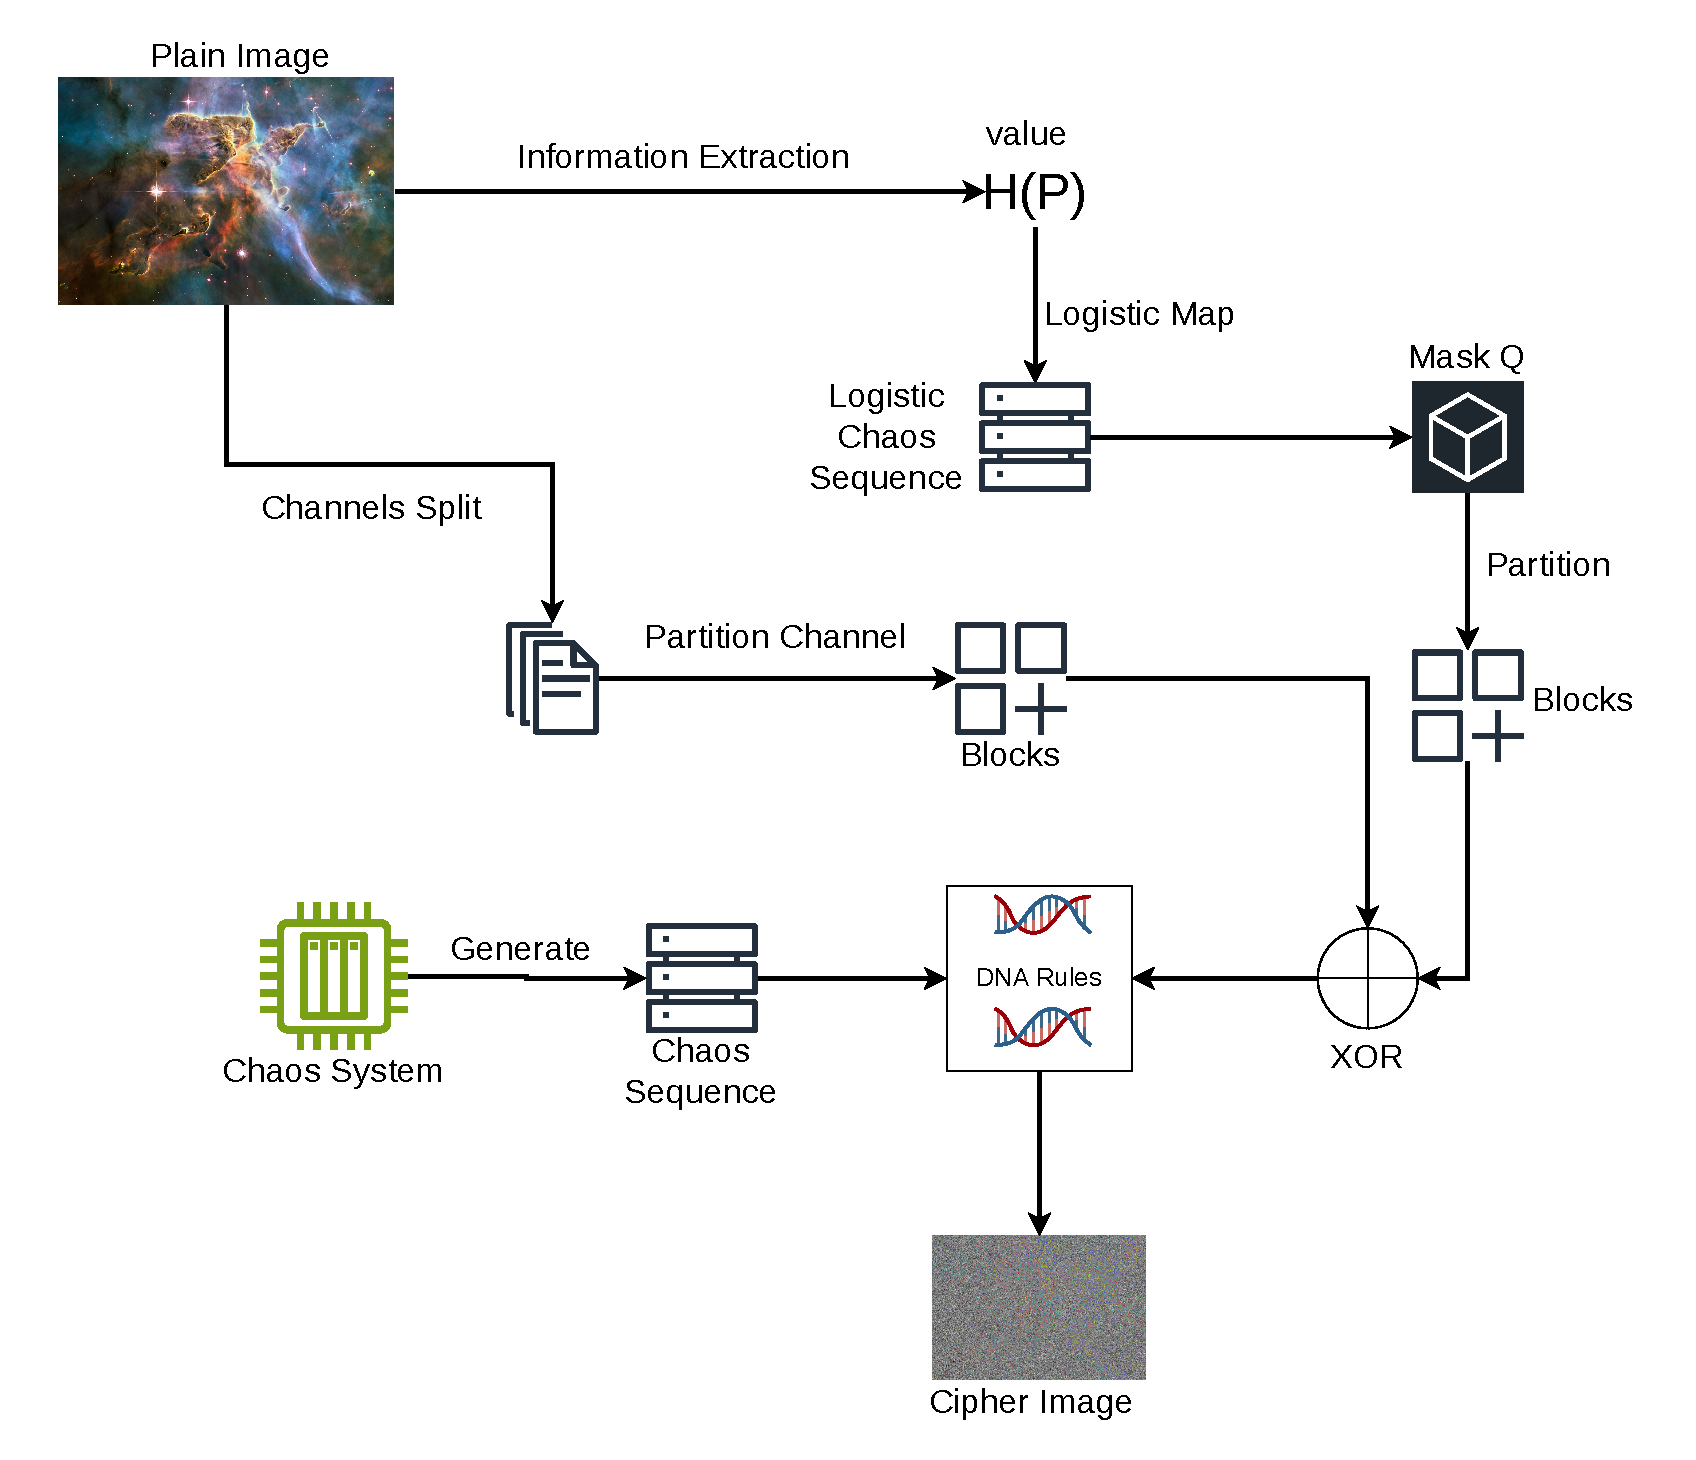
\includegraphics[width=0.85\linewidth,keepaspectratio]{figures/manuscript_a/encrypt_process.pdf}
	
	\caption{Flowchart of the image encryption process.}
	\label{fig:encrypt_process}
\end{figure*}

\begin{enumerate}
	\item 
	Let the plain image be defined as $P \in \mathbb{Z}^{H \times W \times C}_{256}$, where $H$, $W$, and $C$ represent the height, width, and number of channels, respectively. The image is first split into individual channels:
	\begin{equation}
		P_c, \quad c \in \{1, 2, \dots, C\}
	\end{equation}

\item
For each channel $P_c$, it is partitioned into $p \times p$ non-overlapping sub-blocks, with each sub-block having a size of $H_N \times W_N$, satisfying $H = p H_N$ and $W = p W_N$. This reorganization process can be rigorously defined by a tensor transformation $\mathcal{F}: \mathbb{Z}^{H \times W} \to \mathbb{Z}^{p \times p \times D}$, where the output depth is $D = H_N W_N$. The transformation steps are as follows:
\begin{equation}
	\mathbf{X} \xrightarrow{\text{Reshape}} \mathbf{X}_1 \in \mathbb{Z}^{p \times H_N \times p \times W_N}
\end{equation}
\begin{equation}
	\mathbf{X}_1 \xrightarrow{\text{Permute}(1, 3, 2, 4)} \mathbf{X}_2 \in \mathbb{Z}^{p \times p \times H_N \times W_N}
\end{equation}
\begin{equation}
	\mathbf{X}_2 \xrightarrow{\text{Reshape}} \mathbf{Y} \in \mathbb{Z}^{p \times p \times D}
\end{equation}

Applying this transformation to each channel yields:
\begin{equation}
	B_c = \mathcal{F}(P_c), \quad c = 1, 2, \dots, C
\end{equation}

\item
To extract the intrinsic features of the image, the information extractor $\mathcal{H}(P)$ is defined as:
\begin{equation}
	\begin{aligned}
	\mathcal{H}(P) = {} &\Bigg[\sum_{k=1}^{C} \sum_{i=1}^{H} \sum_{j=1}^{W} (P(i,j,k) + 1) \\
	&\quad \times (i \cdot W + j + 1) \times k\Bigg] \bmod M
	\end{aligned}
\end{equation}
where $P(i,j,k)$ denotes the pixel value at the corresponding 3D coordinates.

\item
A dual-input hash mapping is designed to map the encrypted password $S_{\text{password}}$ and the extracted image feature $\mathcal{H}(P)$ into an initial state vector $z_0$:
\begin{equation}
	z_0 = \text{Hash}(S_{\text{password}}, \mathcal{H}(P))
\end{equation}

The vector $z_0$ serves as the initial state for the chaotic system. The Logistic map is employed as follows:
\begin{equation}
	z_{t+1} = \mu z_t(1 - z_t)
\end{equation}
By iterating the Logistic map with $z_0$, a chaotic sequence vector $z_L$ is generated. This sequence is then reshaped to construct the mask matrices $Q$ and $B_Q$:
\begin{equation}
	Q = \text{Reshape}_{H \times W} \left( \lfloor 10^{-4} \cdot z_L \rfloor \bmod 256 \right)
\end{equation}
\begin{equation}
	B_Q = \mathcal{F}(Q)
\end{equation}

\item
The mask matrix is utilized for the pre-diffusion of the image (where $\oplus$ denotes the bitwise XOR operation):
\begin{equation}
	B_c = B_Q \oplus B_c, \quad c = 1, 2, \dots, C
\end{equation}

To achieve comprehensive chained information interleaving across all channels and to resolve the undefined initial diffusion matrix, a circular XOR diffusion mechanism is designed. In the initial stage of the chained diffusion, the pre-diffused matrix of the last channel, $B_C$, is utilized as the initial feedback condition. It is XOR-ed with the first channel $B_1$ to establish a closed-loop diffusion ring:
\begin{equation}
	D_1 = B_C \oplus B_1
\end{equation}

Subsequently, for the remaining channels, the sequential diffusion is strictly executed according to the forward chained rule:
\begin{equation}
	D_c = D_{c-1} \oplus B_c, \quad c \in \{2, 3, \dots, C\}
\end{equation}

Through this circular structure, any minute pixel perturbation in a single channel will be propagated to all channels during the subsequent diffusion and looping process, thereby effectively resisting differential attacks.

\item 
Let $R_i \ (i=1,2,\dots,24)$ represent the set of all $4! = 24$ bijective encoding rules between 2-bit binary symbols and DNA bases, as listed in Table~\ref{tab:dna_rules}, with $R_i^{-1}$ denoting the corresponding inverse decoding process. Unlike traditional DNA encryption schemes that restrict the rule set to the 8 Watson-Crick complementary mappings (which preserve complementary partitions and restrict the induced permutations on $\{00, 01, 10, 11\}$ to an order-8 subgroup isomorphic to $D_4$), the proposed scheme fully utilizes all 24 permutations of the symmetric group $S_4$. This eliminates algebraic invariant subspace vulnerabilities under asymmetric encoding--decoding rounds and expands the rule search space threefold. For the state variable sequences outputted by the chaotic system, the quantization function maps the continuous trajectories into rule index sequences:
\begin{equation}
	s_i = F_{\text{quantize}}(x_i), \quad s_i \in \{1, 2, \dots, 24\}
\end{equation}

\begin{table*}[pos=!t,width=\textwidth]
		\centering
		\caption{Full $S_4$ symmetric DNA coding rules (24 permutations).}
		\label{tab:dna_rules}
		\begin{tabular}{c|cccc||c|cccc}
				\hline
				Rule & 00 & 01 & 10 & 11 & Rule & 00 & 01 & 10 & 11 \\
				\hline
				 1 & A & G & C & T & 13 & C & A & G & T \\
				 2 & A & C & G & T & 14 & C & G & A & T \\
				 3 & T & G & C & A & 15 & C & G & T & A \\
				 4 & T & C & G & A & 16 & C & T & G & A \\
				 5 & C & A & T & G & 17 & G & A & C & T \\
				 6 & G & A & T & C & 18 & G & C & A & T \\
				 7 & C & T & A & G & 19 & G & C & T & A \\
				 8 & G & T & A & C & 20 & G & T & C & A \\
				 9 & A & C & T & G & 21 & T & A & C & G \\
				10 & A & G & T & C & 22 & T & A & G & C \\
				11 & A & T & C & G & 23 & T & C & A & G \\
				12 & A & T & G & C & 24 & T & G & A & C \\
				\hline
		\end{tabular}
\end{table*}
	
\item
Using these index sequences, DNA scrambling is executed. Two sequences are used for each round, resulting in two complete rounds of scrambling across the four sequences to yield the encrypted matrices:
\begin{equation}
	D_c' = R_{s_2}^{-1}(R_{s_1}(D_c))
\end{equation}
\begin{equation}
	D_c'' = R_{s_4}^{-1}(R_{s_3}(D_c'))
\end{equation}

\item
Finally, the inverse tensor transformation is applied to the encrypted matrix to obtain the final encrypted image channels:
\begin{equation}
	C_c = \mathcal{F}^{-1}(D_c'')
\end{equation}

\end{enumerate}

The decryption process is the reverse of the encryption process. With the same password, the same Logistic mask, and the synchronized slave chaotic sequences, the DNA transformations and XOR diffusion can be inverted to recover the original image. Crucially, this requires the response system to reproduce the same quantized rule-index sequences as the drive system. The guard-band quantization scheme (with tolerance $\delta = 0.25$ and resolution $K = 48$) ensures that as long as the synchronization residual satisfies $|\epsilon_i| < 0.25 \cdot \mathrm{span}_i / K$, the receiver reconstructs the identical integer key stream without error.

\subsection{Encryption Results and Security Analysis}

To illustrate the effectiveness of the proposed encryption method, we apply it to a color astronomical image (Hubble Space Telescope, ``Mystic Mountain'' in the Carina Nebula). As shown in Fig.~\ref{fig:full_fig}(a) and Fig.~\ref{fig:full_fig}(b), the encrypted image exhibits a noise-like appearance with no visual resemblance to the original. Fig.~\ref{fig:full_fig}(c) confirms that the decrypted image is pixel-wise identical to the original (MAE~$= 0$, PSNR~$= \infty$), verifying the exact reversibility of the proposed scheme when the correct password and synchronized chaotic key streams are used.

We first examine the key space of the encryption scheme.

A sufficiently large key space is essential to resist brute-force attacks. The proposed encryption scheme involves the following independent key parameters:

\begin{table*}[pos=!t,width=\textwidth]
	\centering
	\caption{Key space composition of the proposed encryption scheme.}
	\label{tab:key_space}
	\begin{tabular}{lcc}
		\toprule
		\textbf{Key Parameter} & \textbf{Precision} & \textbf{Effective Bits} \\
		\midrule
		User password $\to$ SHA-256 hash & 256-bit & 256 \\
		Logistic map parameter $\mu$ & IEEE-754 double & 52 \\
		Hopfield initial conditions (3D) & $3 \times$ double & 156 \\
		Pinning node selection & 3 choices & $\approx$1.6 \\
		\midrule
		\textbf{Total} & & $\approx$\textbf{465 bits} \\
		\bottomrule
	\end{tabular}
\end{table*}

The total key space is approximately $2^{465}$, which far exceeds the internationally recognized security threshold of $2^{100}$ for resistance to exhaustive search attacks. This key space is sufficient to prevent brute-force decryption.

Plaintext sensitivity is then assessed through differential tests.

The number-of-pixels-change rate (NPCR) and unified average changing intensity (UACI) are standard measures of plaintext sensitivity:
\begin{equation}
	\begin{aligned}
	\mathrm{NPCR} &= \frac{1}{M \times N} \sum_{i,j} D(i,j) \times 100\%, \\
	D(i,j) &= \begin{cases} 0 & C(i,j) = C'(i,j) \\ 1 & \text{otherwise}. \end{cases}
	\end{aligned}
\end{equation}
\begin{equation}
	\mathrm{UACI} = \frac{1}{M \times N} \sum_{i,j} \frac{|C(i,j) - C'(i,j)|}{255} \times 100\%
\end{equation}
where $C$ and $C'$ are the cipher images obtained from the original and one-bit-modified plain images, respectively. For an ideal cipher, the theoretical expectations are NPCR~$\approx 99.6094\%$ and UACI~$\approx 33.4635\%$.

\begin{table*}[pos=!t,width=\textwidth]
	\centering
	\caption{NPCR and UACI results (mean over 10 random single-pixel LSB modifications).}
	\label{tab:npcr_uaci}
	\begin{tabular}{lccc}
		\toprule
		\textbf{Metric} & \textbf{R} & \textbf{G} & \textbf{B} \\
		\midrule
		NPCR (\%) & 99.600 & 99.600 & 99.600 \\
		UACI (\%) & 33.346 & 33.374 & 33.320 \\
		\midrule
		\textbf{Mean} & \multicolumn{3}{c}{NPCR = 99.600\%, \quad UACI = 33.347\%} \\
		\bottomrule
	\end{tabular}
\end{table*}

As shown in Table~\ref{tab:npcr_uaci}, both NPCR and UACI values closely match their theoretical expectations across all three color channels, confirming that the proposed scheme exhibits strong diffusion properties and is resistant to differential and chosen-plaintext attacks.

We also examine how decryption responds to a small change in the key.

Key sensitivity measures whether a minimal change in the decryption key leads to complete failure of image recovery. The password-derived Logistic initial value $x_0$ is perturbed by $\Delta x_0 = 10^{-14}$, and the resulting decryption is compared with the correct-key result.

\begin{table*}[pos=!t,width=\textwidth]
	\centering
	\caption{Key sensitivity evaluation results.}
	\label{tab:key_sensitivity}
	\begin{tabular}{lccc}
		\toprule
		\textbf{Decryption key} & \textbf{MAE} & \textbf{PSNR (dB)} & \textbf{Bit HD (\%)} \\
		\midrule
		Correct key $K$ & 0.0 & $\infty$ & 0.000 \\
		Wrong key $K + 10^{-14}$ & 75.90 & 8.82 & 49.994 \\
		\bottomrule
	\end{tabular}
\end{table*}

\begin{figure*}[pos=!t,width=\textwidth]
\centering
	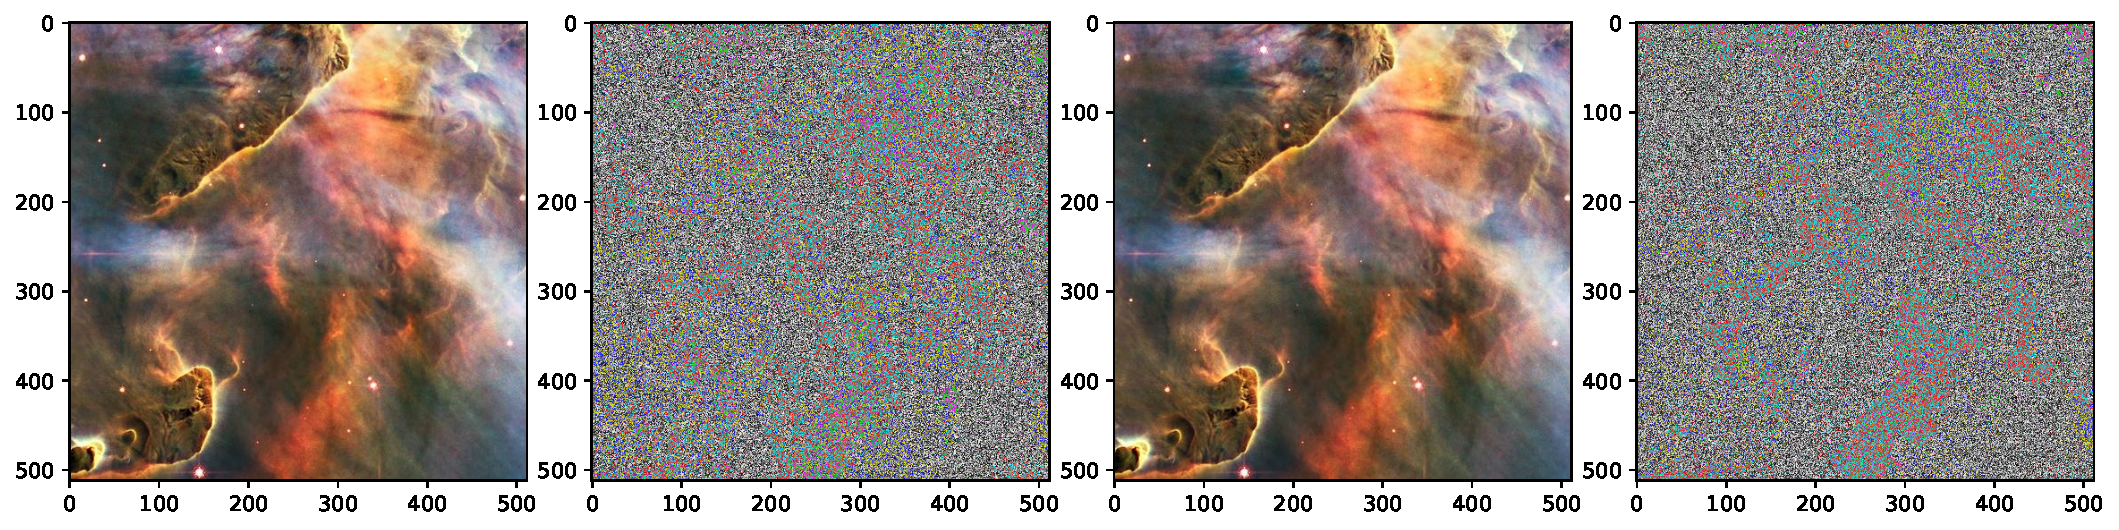
\includegraphics[width=0.95\linewidth]{figures/manuscript_a/key_sensitivity_visual.pdf}
	\caption{Key sensitivity visual comparison. (a)~Plain image. (b)~Cipher image. (c)~Decrypted with correct key (pixel-exact recovery). (d)~Decrypted with wrong key ($\Delta = 10^{-14}$, complete failure).}
	\label{fig:key_sensitivity}
\end{figure*}

As shown in Table~\ref{tab:key_sensitivity} and Fig.~\ref{fig:key_sensitivity}, the correct key produces pixel-exact recovery (MAE~$= 0$), while a perturbation as small as $10^{-14}$ causes complete decryption failure with a bit-level Hamming distance of $49.994\%$---extremely close to the ideal value of $50\%$ expected from a random bit stream. This confirms a strong avalanche effect and demonstrates that the encryption scheme is highly sensitive to the secret key.

The statistical properties of the encrypted image are evaluated using information entropy, histograms, and adjacent-pixel correlations.

The Shannon information entropy measures the randomness of pixel intensity distributions:
\begin{equation}
	H = -\sum_{k=0}^{255} p(k) \log_2 p(k)
\end{equation}
where $p(k)$ is the probability of gray level $k$. For a perfectly uniform distribution, the theoretical maximum is $H = 8$ bits.

\begin{table*}[pos=!t,width=\textwidth]
	\centering
	\caption{Information entropy of the plain and cipher images.}
	\label{tab:entropy}
	\begin{tabular}{lcccc}
		\toprule
		\textbf{Image} & \textbf{R} & \textbf{G} & \textbf{B} & \textbf{Mean} \\
		\midrule
		Plain image & --- & --- & --- & 7.414 \\
		Cipher image & 7.9994 & 7.9993 & 7.9993 & \textbf{7.9993} \\
		Ideal & 8.0000 & 8.0000 & 8.0000 & 8.0000 \\
		\bottomrule
	\end{tabular}
\end{table*}

The cipher-image entropy values in Table~\ref{tab:entropy} are extremely close to the theoretical maximum of 8.0000~bits across all channels, indicating that the encrypted pixel distribution is nearly uniform. This effectively resists statistical analysis attacks based on histogram or frequency analysis.


\begin{figure*}[pos=!t,width=\textwidth]
\centering
	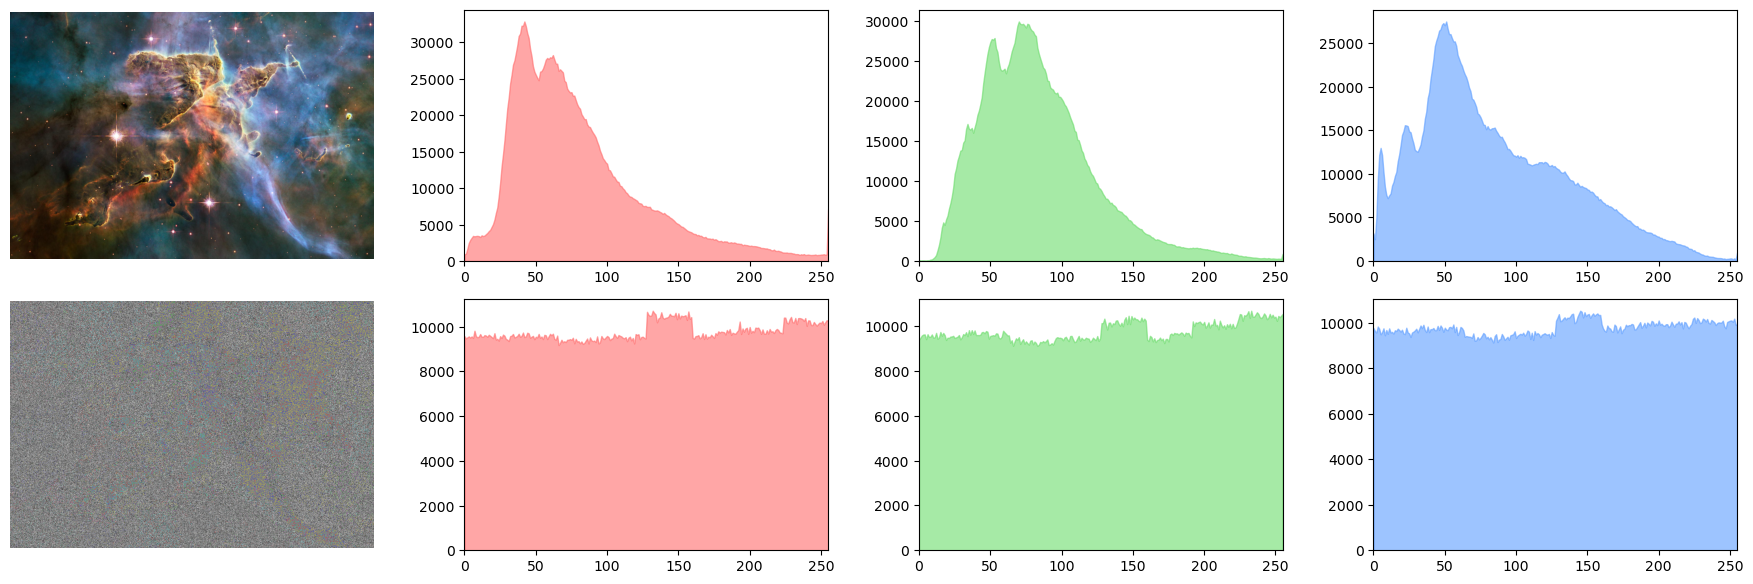
\includegraphics[width=0.9\linewidth]{figures/manuscript_a/test_hist.png}
	\caption{RGB histogram comparison between the plain image and the cipher image.}
	\label{fig:histogram_analysis}
\end{figure*}

The adjacent-pixel correlation coefficient is computed as
\begin{equation}
	r_{xy} = \frac{\operatorname{cov}(X,Y)} {\sqrt{D(X)}\sqrt{D(Y)}},
\end{equation}
where $X$ and $Y$ denote two adjacent-pixel sequences sampled in the horizontal, vertical, or diagonal direction.

\begin{figure*}[pos=!t,width=\textwidth]
\centering
	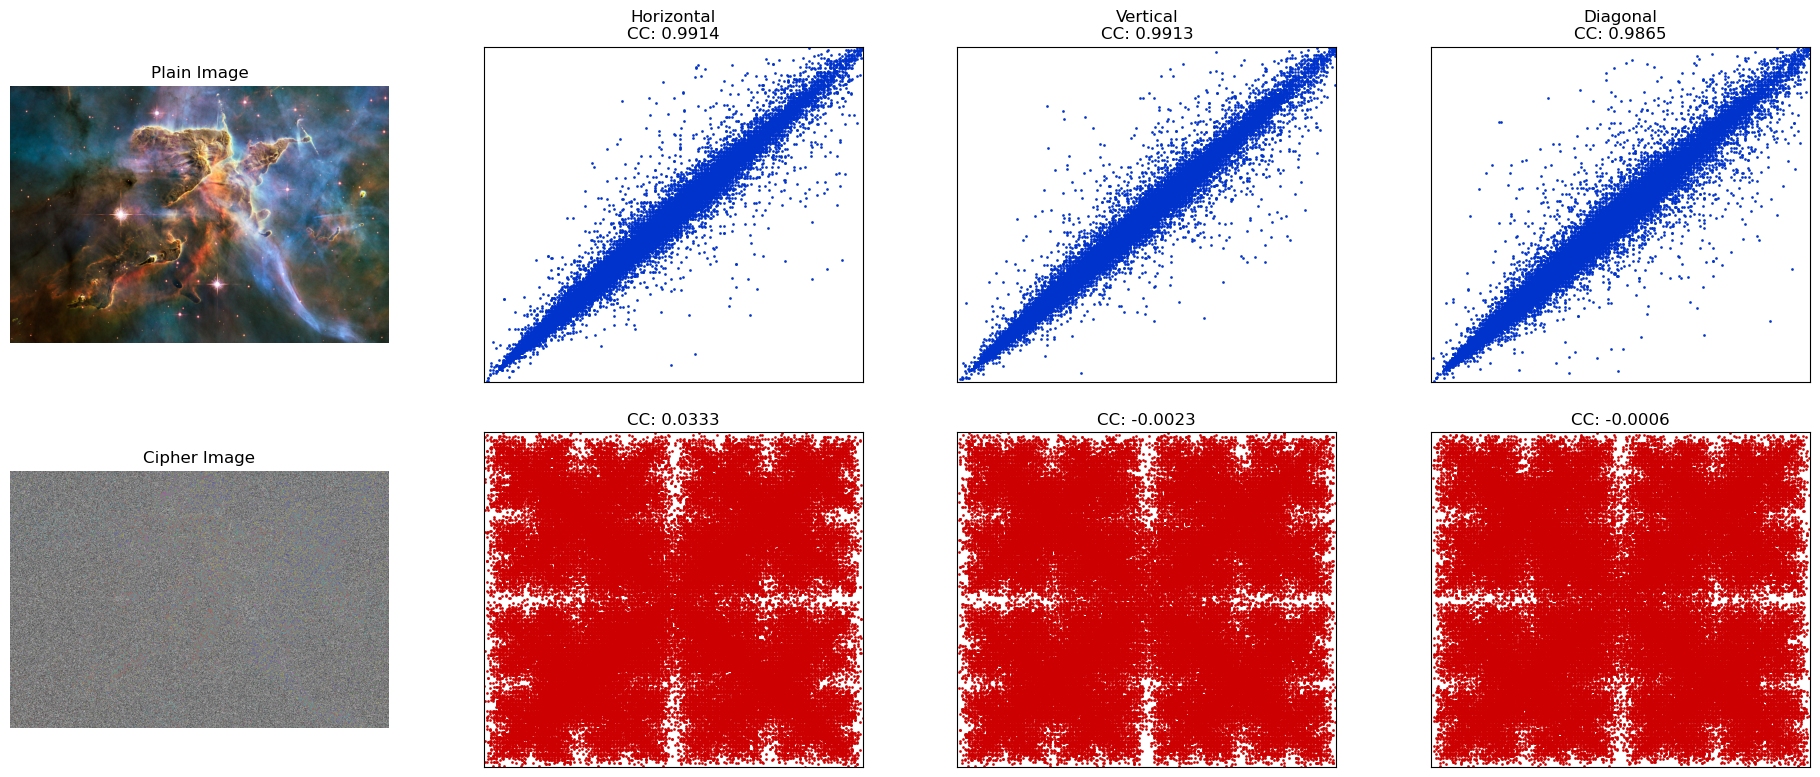
\includegraphics[width=0.9\linewidth]{figures/manuscript_a/test_correlation.png}
	\caption{Adjacent-pixel correlation analysis of the plain and cipher images in horizontal, vertical, and diagonal directions.}
	\label{fig:correlation_analysis}
\end{figure*}

As shown in Fig.~\ref{fig:histogram_analysis}, the histograms of the plain image are highly non-uniform, whereas those of the cipher image are nearly flat across the entire gray-level range. As reported in Table~\ref{tab:correlation_index}, the original images have correlation coefficients close to 1 in all three directions, confirming the strong spatial redundancy of natural images. After encryption, the coefficients decrease to values near 0. The scatter plots in Fig.~\ref{fig:correlation_analysis} further show that the encrypted pixels are broadly dispersed rather than concentrated along the diagonal.

\begin{table*}[pos=!t,width=\textwidth]
	\centering
	\caption{Correlation coefficients of the original and encrypted images.}
	\label{tab:correlation_index}
		\begin{tabular}{lccc}
			\toprule
			\textbf{Image} & \textbf{Horizontal} & \textbf{Vertical} & \textbf{Diagonal} \\
			\midrule
			Original image & 0.9884 & 0.9872 & 0.9772 \\
			Encrypted image (proposed) & 0.0511 & $-$0.0003 & $-$0.0044 \\
			Ref.~\cite{li2024novel} & $-$0.0015 & 0.0023 & 0.0021 \\
			Ref.~\cite{verma2025quantum} & $-$0.0123 & $-$0.0068 & $-$0.0368 \\
			\bottomrule
		\end{tabular}
\end{table*}

Compared with the methods in Refs.~\cite{li2024novel,verma2025quantum}, the proposed scheme achieves comparable correlation suppression in the vertical and diagonal directions, demonstrating its effectiveness in reducing local statistical redundancy.

\subsection{Synchronization Precision and Decryption Reliability}

A key concern raised for synchronization-based encryption is whether the synchronization residual (of order $10^{-2}$) causes decryption errors. To address this, we conduct a controlled experiment: Gaussian noise with varying standard deviation $\epsilon$ is injected into the slave trajectory to simulate different synchronization precision levels, and the resulting decryption quality is measured.

\begin{figure*}[pos=!t,width=\textwidth]
\centering
	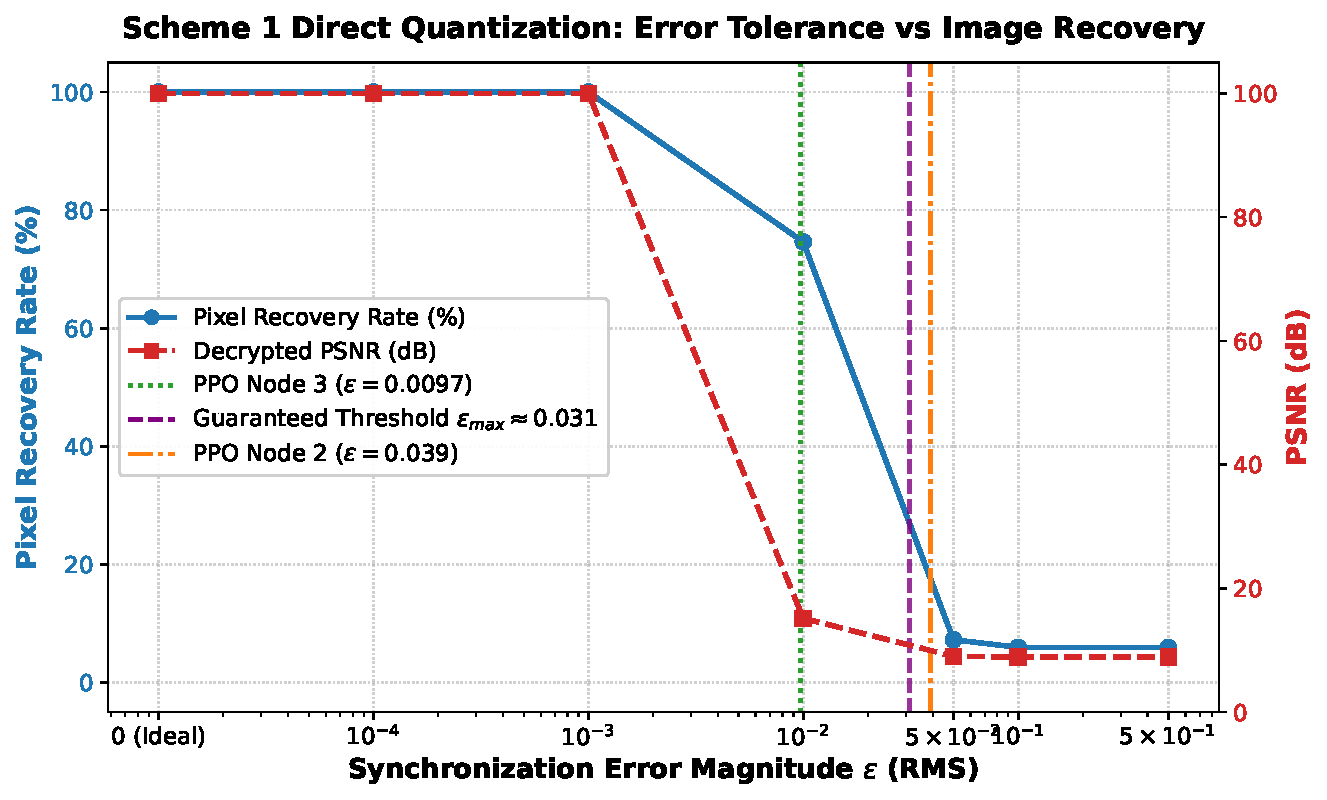
\includegraphics[width=0.85\linewidth]{figures/manuscript_a/sync_error_tolerance_curve.pdf}
	\caption{Synchronization error tolerance curve. Left axis: pixel recovery rate. Right axis: decrypted PSNR. Vertical lines mark the PPO Node~3 operating point ($\epsilon \approx 0.0097$), the theoretical guard-band threshold ($\epsilon_{\max} \approx 0.031$), and the Node~2 operating point ($\epsilon \approx 0.039$).}
	\label{fig:sync_error_curve}
\end{figure*}

As shown in Fig.~\ref{fig:sync_error_curve}, the quantization guard-band mechanism provides complete error-free decryption for synchronization residuals below $10^{-3}$. A steep transition occurs in the range $\epsilon \in [10^{-2}, 5 \times 10^{-2}]$, beyond which decryption fails entirely. The theoretical maximum tolerable state residual is $\epsilon_{\max} = \delta \cdot \mathrm{span} / K \approx 0.031$, where $\delta = 0.25$ is the guard-band width and $K = 48$ is the quantization resolution. The PPO Node~3 controller achieves a steady-state synchronization error of approximately $0.0097$, which lies well within the safe region with a margin of approximately $3.2\times$. This result confirms that the reported synchronization precision of order $10^{-2}$ does not cause decryption errors under the proposed quantization scheme, and the guard-band mechanism effectively bridges the gap between continuous-domain synchronization residuals and discrete-domain key-stream consistency.


\section{Conclusion}
\label{sec:conclusion}

This study developed a PPO-based single-input pinning framework for synchronization of a continuous-time Hopfield chaotic neural network. Local control indicators guided the comparison of actuator locations, while the bounded-input analysis established state boundedness and the post-training numerical assessments examined local perturbation decay. The experiments show that synchronization performance depends jointly on the controlled node and the observed variables: observation subsets of equal dimension can produce markedly different errors and energy requirements, and the targeted SAC comparison reproduces the direction of the tested error changes. Comparisons across actuator subsets further quantify the cost of restricting control to one node. Single-input Node 3 achieves low residuals with less total control energy than the favorable multi-input configurations, whereas additional inputs improve full-horizon accuracy. Together with the traditional-controller benchmarks, these results support selecting actuator location and observation content according to the required accuracy and available control resources.

The synchronized trajectories were also used in an image-encryption and decryption application combining Logistic-map masking and dynamic DNA coding. The reported reconstruction and image-statistics tests examine the use of the learned synchronization controller beyond the continuous-state control task, while the synchronization-precision experiment connects residual error with discrete decryption performance. This application highlights the need to evaluate synchronization against the requirements of the downstream task, rather than relying on an average error alone. Future work will extend the control comparisons to other network parameters and combined disturbances, develop explicit synchronization-error bounds, and further assess the encryption scheme under realistic communication and attack conditions.

\section*{Declaration of competing interest}
The authors declare that there is no conflict of interest regarding the publication of this paper.

%

\section*{Data availability}
The data that support the findings of this study are available from the corresponding author upon reasonable request.

%% Loading bibliography style file
%\bibliographystyle{unsrtnat}
\bibliographystyle{elsarticle-num}
%\bibliographystyle{model1-num-names}
%\bibliographystyle{cas-model2-names}

% Loading bibliography database
\bibliography{ref_A}

\end{document}
